
\chapter{The rise of Peripheral Swedish: Reconstructing a plausible scenario}
\section{General}
\label{sec:6.1}

In what precedes, we have been looking at a number of innovative linguistic phenomena that are spread over large, partly non-contiguous, geographic areas. If a particular linguistic phenomenon is found in two or different members of the same language family but did not exist at earlier historical stages of that family, there are a number of logical possibilities for how such a situation could arise:  

\begin{enumerate}
\item  
There is no causal connection between the different manifestations of the phenomenon; it has developed quite independently in the various locations where it is found. 
  
\item  
The developments are in principle independent of each other, but are triggered by the same internal factors which are due to shared properties inherited from their common ancestor. 
 
\item  
The phenomenon is due to a common development. This is compatible with a variety of scenarios: the spread may have taken place through migration of speakers, or through influence from a cultural and economical centre, or through a vaguer process of dissipation, without any well-defined centre of origin. 
\end{enumerate}

%\end{styleListeii}

%\end{listLFOxvleveli}

Obviously, possibilities 2 and 3 shade into each other: if people in two close-by communities suddenly seem to get the same idea, it is not always possible to tell if they have influenced each other or if they are inspired by the same situation. 

To see how one could argue for or against the different possibilities, let us look at one of the central processes discussed above, the extension of the use of definite forms to contexts which are not usually seen as definite. Is it, to begin with, possible that this development could have taken place independently, say, in Dalarna, Upper Norrland, and Finland? 

One issue that has bearing on this question is the general typological probability of the development in question. Definiteness marking is found in many languages all over the world; we also know that it is not uncommon for definiteness markers to generalize in such a way that they no longer deserve that name. However, it does appear that developments that parallel the Scandinavian ones more closely are not so common – otherwise they ought to have attracted the attention of typologists to a greater extent. In \sectref{sec:3.2.3.2}, we saw a fairly close parallel in Moroccan Arabic and certain less clear tendencies among the Romance languages. Among the Germanic languages, nothing similar has been attested so far. These facts certainly speak against the assumption that the parallels between Dalarna, Upper Norrland and Finland are coincidental. But could there be factors that would favour a parallel development without there being a direct spread of innovations? One point of some importance here is that Scandinavian definiteness marking has reached a relatively “advanced” stage of grammaticalization in that it involves affixation and sometimes fusion between stem and affix, rather than the article being a free morpheme, which is the case in most European languages that have a definite article. It is likely that the further expansion of the definite article to, for instance non-delimited uses, is easier if the article is bound than if it is free. (The Arabic definite article is written orthographically as a separate word but in the spoken dialects, such as Moroccan Arabic, it is actually more like an affix.) 

Could the innovations in Peripheral Swedish noun phrase syntax be due to a common spread from a centre? The obvious problem is to identify this centre, given that the phenomena that we are examining in several cases are found in discontiguous areas and that there is no common economic and cultural centre within their present-day territory. We do not have go very far to find such a centre outside the Peripheral Swedish area, however, as is suggested in the following quotation: 

%\begin{styleBlockQuote}
“The Norrlandic and East Swedish [i.e. Trans-Baltic] dialects are in general ramifications of the Upper Swedish area. They hardly have any centre of their own, but point to Central Sweden, especially Uppland, as their original middle point. However, in these more peripheral dialect groups, several traits have been retained that have been pushed out from central Sweden by innovations from the south or by influence from the standard language.” (\citet[51]{Wessén1966}, my translation)

%\end{styleBlockQuote}

Wessén seems here to be speaking of the retainment of conservative traits in the Peripheral Swedish area. It is natural to think of those traits as being inherited from Old Nordic, and to assume that they were once found in the whole Scandinavian linguistic area. In actual fact, the feature Wessén uses as an illustration in the same chapter – “vowel balance” – is not of this kind. Like another feature he mentions earlier in the book – “medial affrication” – vowel balance is an innovation that was never characteristic of all Scandinavian varietes.  However, these features still covered a larger area in earlier times than they do today – particularly in parts of the central provinces of Uppland and Södermanland.” The “innovations from the south” that have pushed them out are thus not really innovations but rather a return to an original state; that is, the varieties that win out are the more conservative ones – at least as far as these particular developments go. Let us look at the details.

“Medial affrication” (in Swedish literature often referred to as \textstyleLinguisticExample{norrländsk förmjukning} ‘Norrlandic softening’) is the process that gives rise to forms such as Elfdalian \textstyleLinguisticExample{mjotje}; ‘the milk’, where the stem-final \textstyleLinguisticExample{k} in \textstyleLinguisticExample{mjok} ‘milk’ has become a [tʃ] before the front vowel in the definite ending. This is different from the palatalization of \textstyleLinguisticExample{k} and \textstyleLinguisticExample{g} before stressed vowels that is found in most spoken varieties of Peninsular Scandinavian, including Standard Swedish and Norwegian. Medial affrication is usually described as applying generally in Swedish vernaculars north of a line more or less coinciding with \textstyleLinguisticExample{limes norrlandicus,} including parts of Swedish-speaking Finland (but not Estonia). In addition, it is also found in most of western and northern Norway. \figref{map:22} shows the borderlines of the medial affrication area according to \citet{Haugen1970}, which, like most other treatments, shows the border through Uppland as described in \citet{Kruuse1908}; this mapping may be assumed to represent the second half of the 19\textsuperscript{th} century. In \citet{KällskogEtAl1993}, the phenomenon is said to be “extremely rare” in Uppland except in the very north and is judged by the editors of the volume to be disappearing in this province – the only attestation in the texts in the book is from the parish of Hållnäs. 

\begin{figure}[h]
 
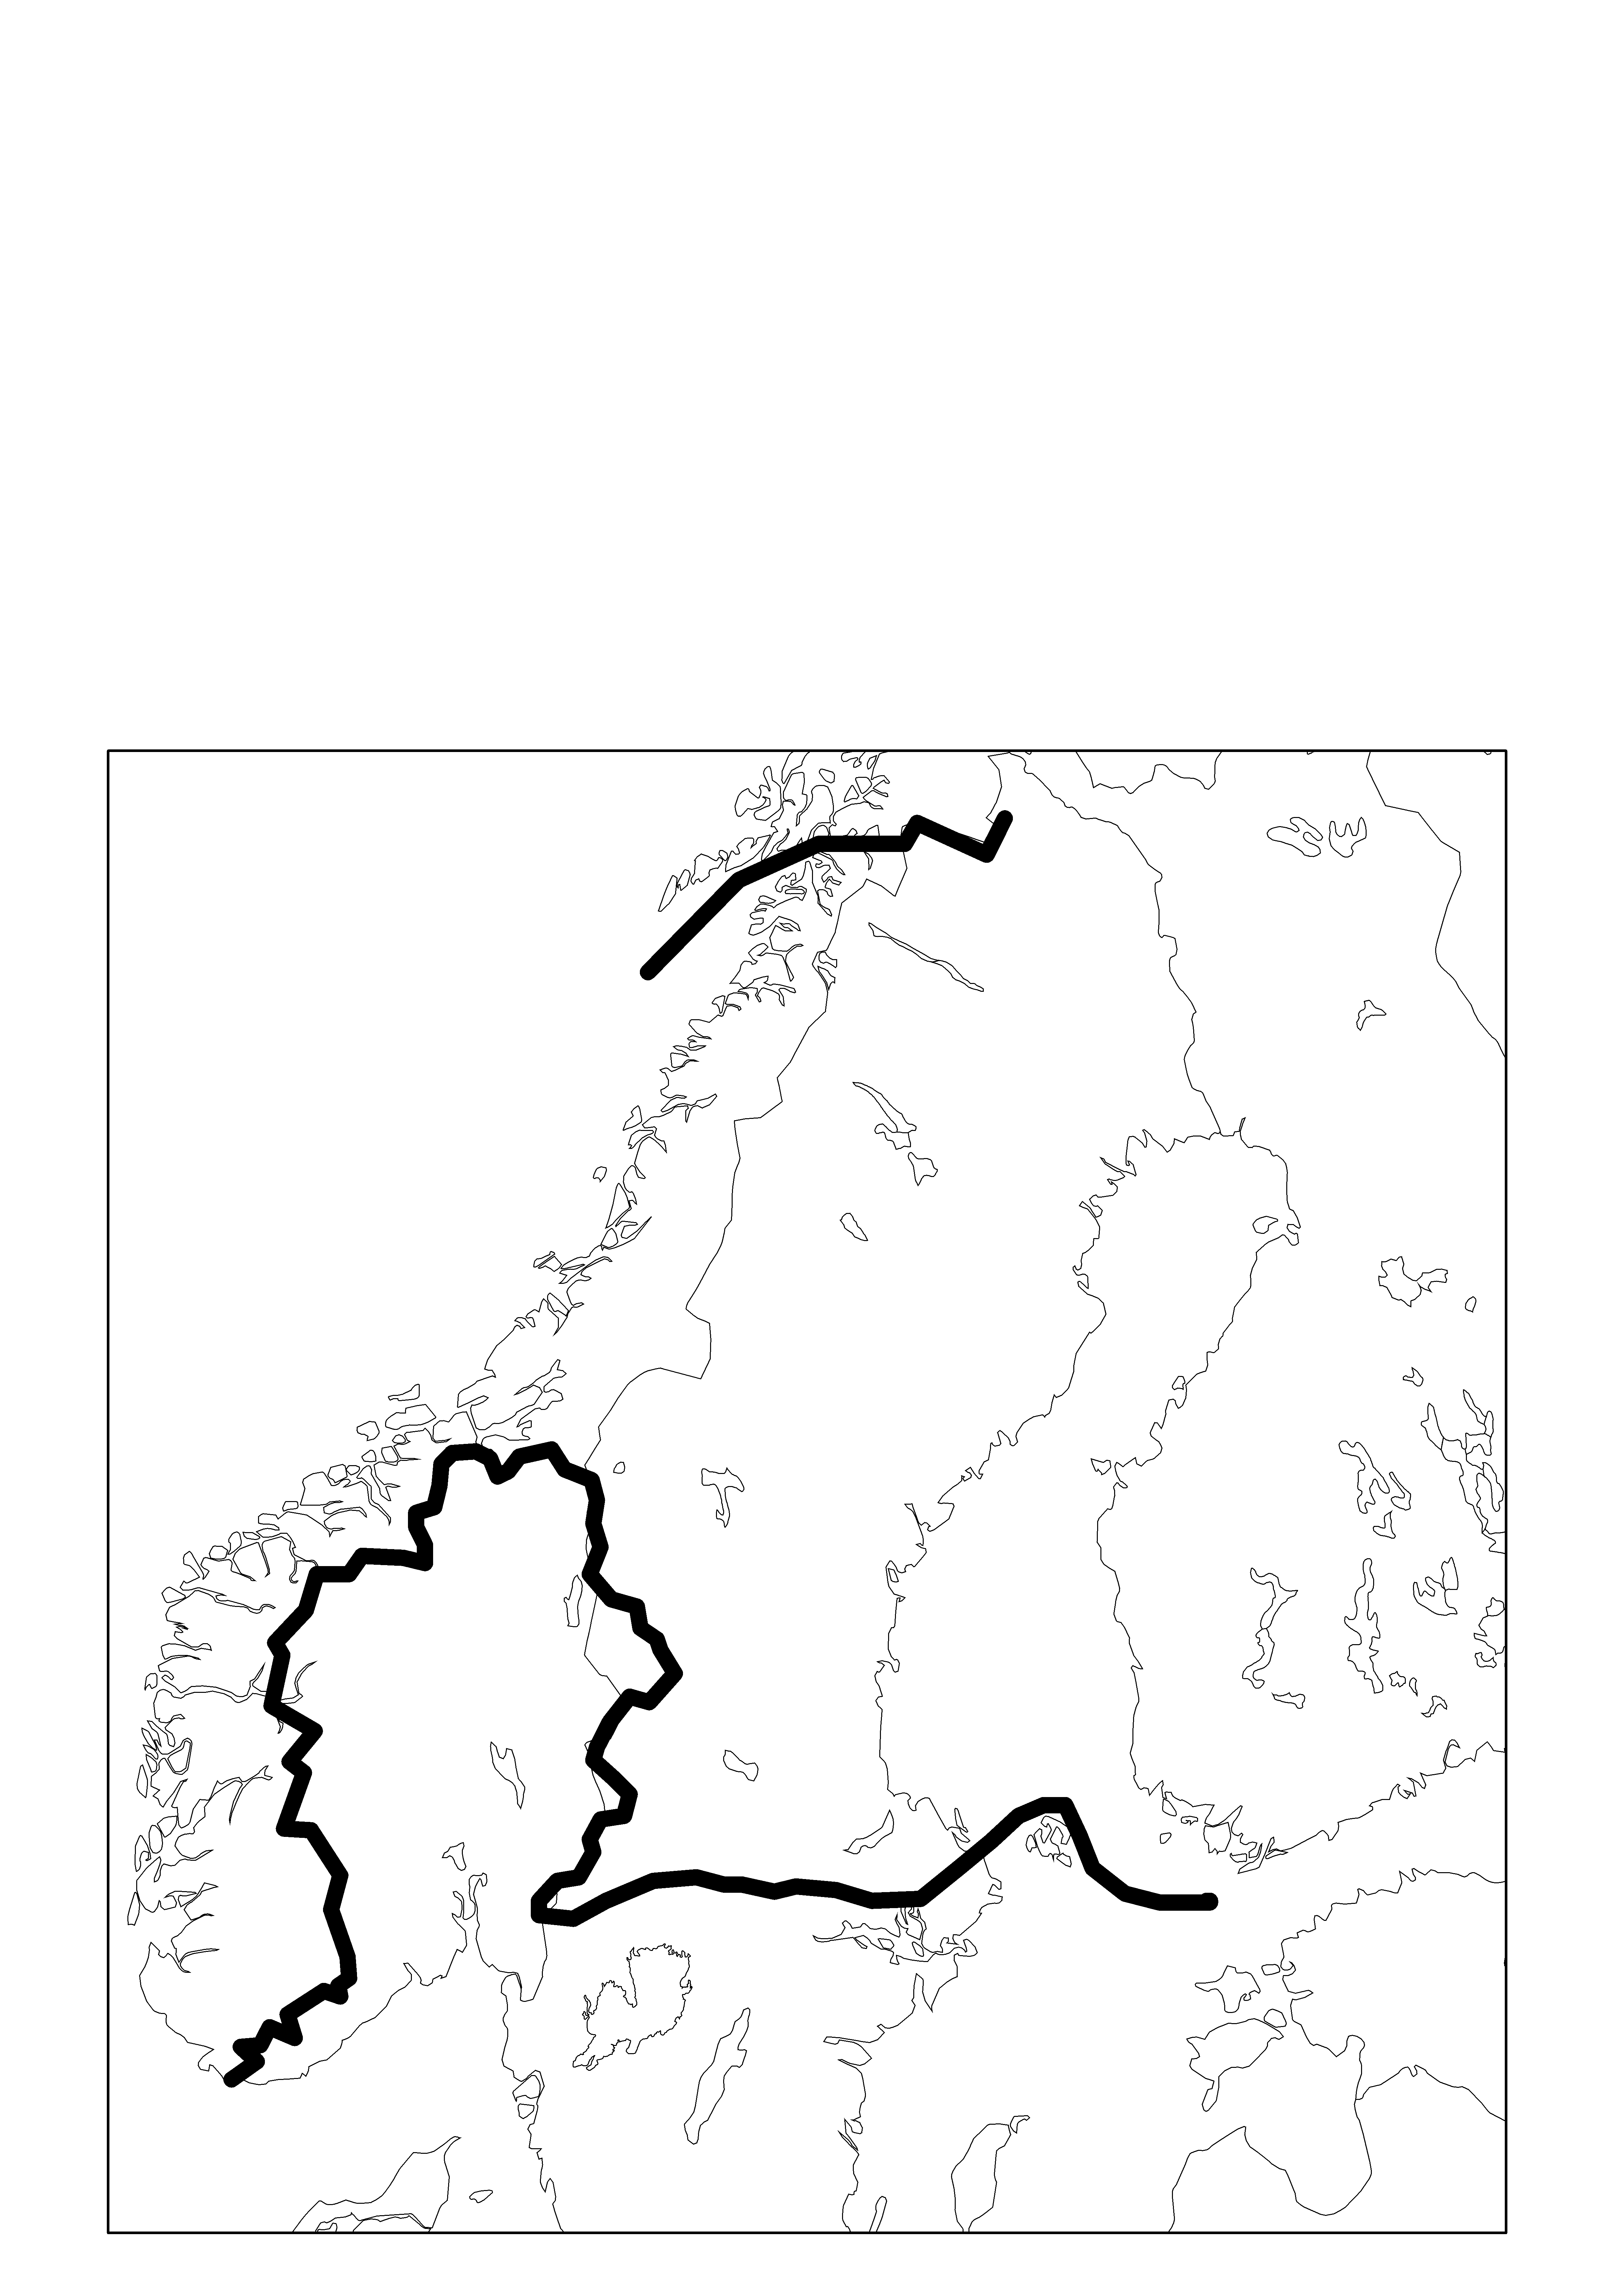
\includegraphics[height=.5\textheight]{figures/26_BorderlinesofMedAf}
\caption{The borderlines of medial affrication according to \citet{Haugen1970}}
\label{map:22}

 
\end{figure}

\citet[43]{Wessén1966} says that there is evidence that medial affrication earlier covered a larger area, extending also to parts of Södermanland and the archipelago along the coast of Östergötland. (The footnote in \citet[36]{Hesselman1905} which Wessén refers to says “all of eastern Västmanland, parts of Södermanland”.) \citet{GeijerEtAl1930} demonstrated that sporadic occurrences of medial affrication were found in a large area in Västmanland south of the present borderline, again suggesting a wider distribution in the past. In other words, there appears to be a continuous receding movement northwards. \citet[80]{Reinhammar2005} says that forms such as \textstyleLinguisticExample{bättjen} and \textstyleLinguisticExample{väddjen}, which are known from northern Uppland and northwards, may have spread from Uppland and may also have existed further south, but were pushed out by the forms without affrication “which have as it were regained territory from the south”.

The term “vowel balance” refers to the interdependence in length between a stressed syllable and a following unstressed one that characterizes many northern Scandinavian varieties, due to developments in the Middle Ages; this means in practice that unstressed vowels that followed a short stressed syllable were not subject to the reduction processes that hit other unstressed vowels, thus Written Medieval Swedish \textit{faþir }‘father’\textit{ }({\textless}Runic Swedish\textit{ faþer)} vs. \textit{m}\textit{\=oþ}\textit{er} ‘mother’.  In the varieties where vowel balance has been operative, it is hard to distinguish this as a phenomenon different from apocope, that is the deletion of unstressed final vowels, and “vowel leveling”, that is the assimilation of the quality of the stem vowel to that of the non-deleted but raised final vowel. Thus, in Elfdalian, verbs with original long-syllabic stems show up with the infinitive ending\textit{ {}-a}, which is however apocopated in many positions, e.g. \textstyleLinguisticExample{jag(a)} ‘hunt’ (long stem vowel), whereas short-syllabic stems get the ending\textit{ {}-å} or\textit{ {}-o}, which is never apocopated and also colours the stem vowel, e.g. \textstyleLinguisticExample{båkå{\textless}baka} ‘bake’ (short stem vowel). The geographic distribution of these features is quite complex and I shall not try to disentangle it here. It should be noted, however, that similar processes seem to have been common in large parts of the Germanic area, and it is not easy to reconstruct interrelationships between different varieties. Vowel balance is more directly preserved in Swedish varieties in Dalarna and southern Norrland (except Hälsingland and Gästrikland) but also in the neighbouring Norwegian varieties, covering most of Eastern Norway. In addition, it shows up in Finland and Estonia. Curiously enough, although medial affrication and vowel balance are strongly positively correlated in the Swedish dialect area, their distribution in Norway is almost perfectly complementary. \citet[52]{Wessén1966} notes: “There are many traces of vowel balance also in Upper Swedish dialects, and it does appear that this regulation of final vowels earlier extended south to the border to the Göta area.” Apocope was also apparently common in older forms of Upper Swedish (\citet{Wessén1968}).

What I want to show now is that there is in fact a fairly large number of other phenomena, both grammatical and lexical, that show similar patterns, that look like innovations that have been pushed back. I will also try to show that the geographical distribution of those innovations tends to resemble that of truly conservative features that have also been pushed back, which suggests a relatively early date for the innovations in question.

\section{Pushed-back innovations in the pronoun system}

Some of the most important innovative phenomena in the Peripheral Swedish area belong to the pronoun systems. Their distribution in time and space has been studied in detail by the late Swedish dialectologist Vidar Reinhammar (especially \citet{Reinhammar1975}). 

\subsection{\textit{H}{}- and \textit{d}-pronouns}

The term “\textstyleLinguisticExample{h-}pronouns” is here used as a convenient label for demonstrative and 3\textsuperscript{rd} person pronouns formed from stems beginning in \textstyleLinguisticExample{h}, as opposed to “\textstyleLinguisticExample{d-}pronouns” whose stems begin in a dental. This should not be taken as implying that \textstyleLinguisticExample{h-}pronouns all have a common origin. Nevertheless, this label nicely covers the innovative pronouns in the Peripheral Swedish area.

\subsection{Adnominal \textit{h-}pronouns}

In Central Scandinavian, the pronouns \textstyleLinguisticExample{han} ‘he’ and \textstyleLinguisticExample{hon} ‘she’ are not used adnominally. By contrast, in many vernaculars throughout the Peripheral Swedish area, masculine \textstyleLinguisticExample{han} and feminine \textstyleLinguisticExample{hon} form a paradigm of adnominal demonstratives together with neutral \textstyleLinguisticExample{hä, }with the plural taken from the \textstyleLinguisticExample{d-}series, as in the neuter dative forms\textstyleLinguisticExample{. }In Elfdalian, we thus have the nominative forms \textstyleLinguisticExample{an kalln} ‘that man’, \textit{o}[328?]\textstyleLinguisticExample{ kulla} ‘that woman’, \textstyleLinguisticExample{eð auseð} ‘that house’, \textstyleLinguisticExample{dier kallär} ‘those men’, and the neuter dative form \textstyleLinguisticExample{dyö ause; }‘that house’. The geographical distribution is shown in \figref{map:23}. 

There are no attested examples of adnominal \textstyleLinguisticExample{h-}pronouns in Written Medieval Swedish (\citet[114]{Reinhammar1975}). The innovation must have taken place during the Middle Ages, but it is unclear if it had already happened during the “Early Old Swedish” period (ibid.).

Reinhammar reconstructs the following area for the maximal geographical distribution of adnominal \textstyleLinguisticExample{h-}pronouns: in addition to the present-day area, he assumes that \textstyleLinguisticExample{han} and \textstyleLinguisticExample{hon} were used more extensively in eastern Uppland, possibly also in eastern Södermanland (the Södertörn peninsula\footnote{ Södertörn is the triangular peninsula directly south of Stockholm. It is best visible in \figref{map:40}.}). Similarly, adnominal \textstyleLinguisticExample{hä }was also used in SE Uppland and possibly in Södermanland, in addition in Öland and Gotland. 

Reinhammar sees adnominal \textstyleLinguisticExample{han/hon }in Uppland, Estonia, Åland, Åboland, western Nyland, and northern and southern Österbotten as forming a unitary area, to which Öland would also belong. The innovation centre was probably Uppland and the innovation spread “along coasts and via water-ways” (\citet[115]{Reinhammar1975}).

“From the point of view of dialect geography” it can be assumed, says Reinhammar, that the Swedish east coast from Södertörn to Öland had adnominal \textstyleLinguisticExample{han/hon} during some period and that it was later pushed out by \textstyleLinguisticExample{d-}pronouns. Åland has “undoubtedly” had \textstyleLinguisticExample{han/hon, }although mainland Åland has shed it due to influence from the standard language. As for Österbotten, the adnominal \textstyleLinguisticExample{h-}pronouns can be assumed to have arrived via “the Swedish settlements in Satakunta” (the province south of Österbotten, presently only Finnish-speaking) rather than directly from Sweden, “since the Norrlandic dialects do not know the use in question and the distance to Uppland seems too large” (\citet[116]{Reinhammar1975}). The situation in Österbotten is complicated by the existence of an alternative pronoun paradigm \textstyleLinguisticExample{tan}, \textstyleLinguisticExample{ton} – I will not go into Reinhammar’s discussion of these problems. 

Concerning the use of adnominal \textstyleLinguisticExample{h-}pronouns in Dalarna, Reinhammar says that it is “less probable” that it has arisen as an internal development with no relation to the large area mentioned above. Although “it cannot be excluded” that the \textstyleLinguisticExample{h-}pronouns entered Dalarna through a colonization from Uppland, Reinhammar prefers to see the two areas as “remnants of an older unity”. (Apparently Reinhammar sees these alternatives as excluding each other.) He refrains from taking a definite view on the extension of this unified area but conjectures that it may have, in addition to the Dalecarlian area, also been comprised of parts of Uppland, eastern Västmanland and southern Dalabergslagen, and perhaps a part of Gästrikland. Now the problem arises as to how to explain the “intermediary area” where adnominal \textstyleLinguisticExample{h-}pronouns are not found today. Reinhammar speculates that the spread could have taken place through a “pincer operation” but says that, in any case, we must assume that the \textstyleLinguisticExample{d-}pronouns have regained part of the territory that they earlier lost to the \textstyleLinguisticExample{h-}pronouns. From Reinhammar’s rather lengthy discussion of this issue, I will just mention his claim that the competition between \textstyleLinguisticExample{d-} and \textstyleLinguisticExample{h-}pronouns in the Dalecarlian area may be explained by the hypothesis that the innovation was never fully implemented there. 

Adnominal \textstyleLinguisticExample{hä }has a larger distribution than adnominal \textstyleLinguisticExample{han/hon, }and is in fact combined with non-neuter \textstyleLinguisticExample{den} in one paradigm in an area comprising parts of Uppland, Västmanland, Dalabergslagen and Gästrikland (\figref{map:23}). “It does not seem unlikely” that this area earlier had a full \textstyleLinguisticExample{h-}pronoun paradigm (\citet[43]{Reinhammar1975}. Combinations of \textstyleLinguisticExample{h-}pronouns with the deictic adverb \textit{dar/dä}r also occur in a wider area (\figref{map:24}); in Standard Swedish, only \textit{d}{}-pronouns are normally possible.   
 
 
 

\begin{figure} 
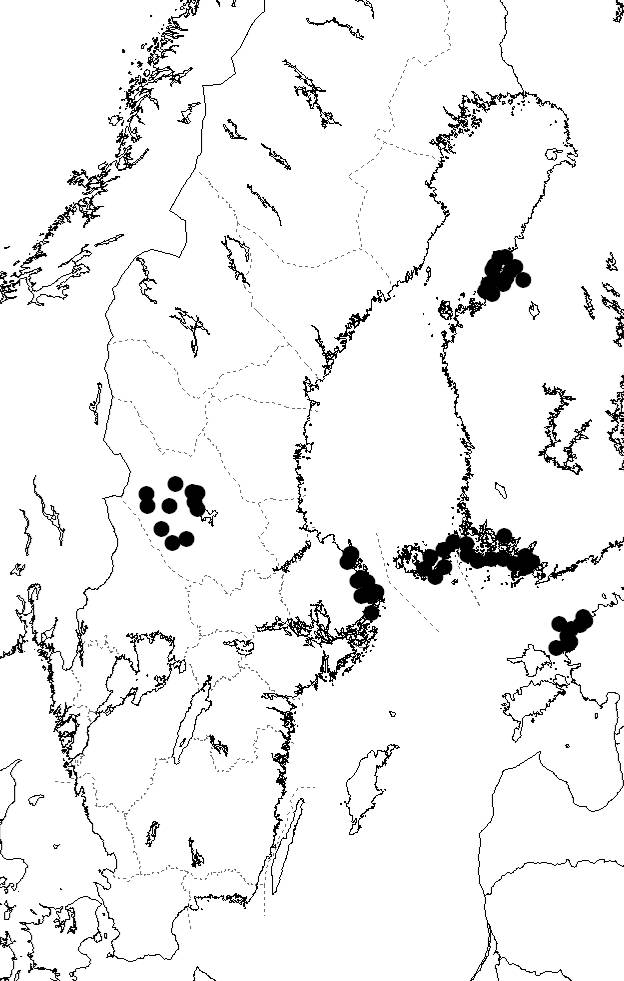
\includegraphics[height=.5\textheight]{figures/27_Adnominalmasculine}
\caption{Distribution of adnominal masculine \textit{h-}pronouns without adverbial expansions (Reinhammar’s \figref{map:4}).}
\label{map:23}
\end{figure}

\begin{figure}  
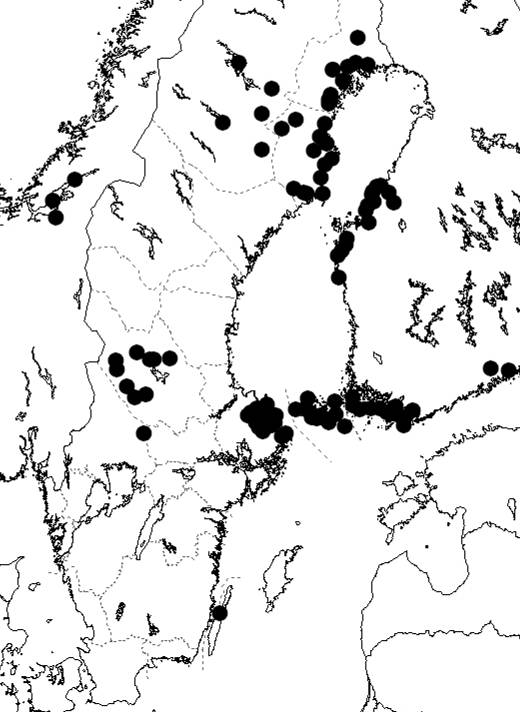
\includegraphics[height=.5\textheight]{figures/28_AdnominalmasculineDar}
\caption{Distribution of adnominal masculine \textit{h-}pronouns in combination with \textit{dar} (Reinhammar’s \figref{map:5}).}
\label{map:24}
\end{figure}
 
\begin{figure} 
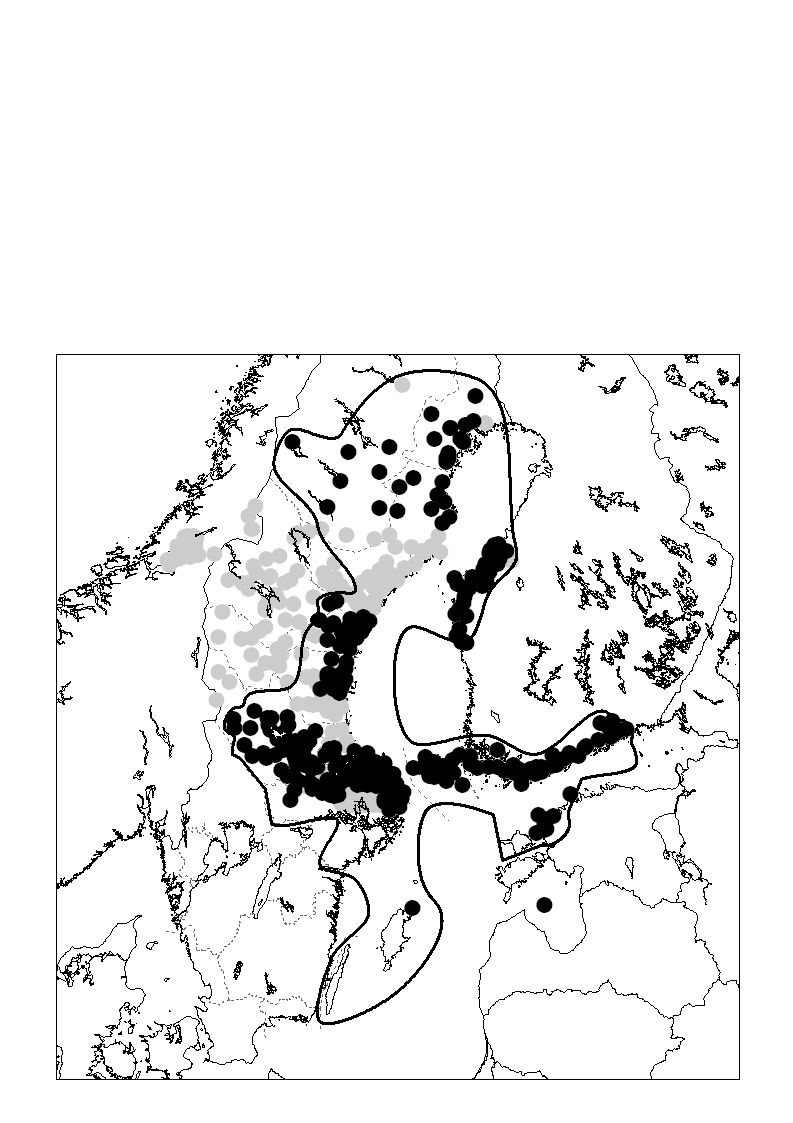
\includegraphics[height=.5\textheight]{figures/29_StressedandEnclitic}
\caption{Modern distribution of stressed and enclitic independent \textstyleLinguisticExample{hä} (black and grey circles, respectively) and reconstructed maximal extent of stressed \textit{hä} (enclosed area).}
\label{map:25}  
\end{figure}

\subsection{Independent \textit{hä}}

Forms such as \textstyleLinguisticExample{hä}, \textstyleLinguisticExample{ä, äd}, etc. are widely used as independent neuter pronouns in the Peripheral Swedish area. For simplicity, I shall refer to all these forms simply as \textstyleLinguisticExample{hä}. \figref{map:25} shows the present-day distribution of the stressed variants. 

Reasoning out from dialect geography and older materials, Reinhammar deems it probable that \textstyleLinguisticExample{hä} was earlier used in a contiguous area comprising Norrbotten, Västerbotten and the present-day \textstyleLinguisticExample{hä}{}-areas in Lappland (to the extent that they were populated), eastern Ångermanland, Medelpad (except Haverö) and the easternmost corner of Jämtland, Hälsingland except the north-west, Dalarna except in north-west, Gästrikland, Uppland, Västmanland except possibly the south-western part, (at least) northern and eastern Södermanland, and possibly also Närke and the north-east corner of Östergötland. In addition \textstyleLinguisticExample{hä} existed in Öland, (the whole of) Gotland, and generally in Finland and Estonia. Reinhammar does not exclude the possibility that the use of \textstyleLinguisticExample{hä} was less general in some of the areas where it later receded, but says that the most probable assumption is that a relatively uniform system was prevalent as least as far as stressed and proclitic uses are concerned.

The Swedish mainland \textstyleLinguisticExample{hä}{}-area has been split up or “otherwise decreased in extent”. The corresponding \textstyleLinguisticExample{d-}form, denoted as \textstyleLinguisticExample{dä} (corresponding to standard orthography \textstyleLinguisticExample{det}), has expanded “mainly from the south and partly from Stockholm” and replaced \textstyleLinguisticExample{hä} in Södermanland, SE Västmanland, S Uppland, “also infiltrating remaining \textstyleLinguisticExample{hä}{}-vernaculars in Uppland and NE Västmanland, as also partially in Dalabergslagen and Gästrikland” (\citet[186]{Reinhammar1975}). A similar process has taken place in Finland, affecting Åland (from the Swedish mainland) and Nyland (from Helsinki) (\citet[187]{Reinhammar1975}).

For Hälsingland, Reinhammar assumes a spread along the rivers Ljusnan and Voxnan and the coast in the south-west. Northwestern Hälsingland, on the other hand, belongs to an area with original \textstyleLinguisticExample{dä}, comprised of Härjedalen, Jämtland and W Medelpad (that is, areas under Norwegian influence – my remark) (\citet[186]{Reinhammar1975}). For Ångermanland, the picture seems to be somewhat confused – Reinhammar mentions several possibilites but does not want to choose between them. In Gotland, the reconstituted \textstyleLinguisticExample{dä} can be assumed to have spread from Visby (\citet[188]{Reinhammar1975}). 

Finally, Reinhammar raises the questions of the age of \textstyleLinguisticExample{hä} and how its large distribution should be explained. He notes that early attestations of \textstyleLinguisticExample{hä} are found over a large area, such as Gotland from about 1550, Älvdalen from about 1600, and Uppland from 1620. This is an indication of an early spread. Reinhammar says that \textstyleLinguisticExample{hä} should be seen as having originated in the Old Swedish period (i.e. before 1520), “maybe already in the latter part of the Early Old Swedish period”.\footnote{ “Häd, äd bör därför antas ha sin upprinnelse i fsv. tid, kanske redan i senare delen av äldre fsv.” (\citet[189]{Reinhammar1975}).} Since the period of Early Old Swedish is normally given as 1225-1375, this should be interpreted as meaning the three first quarters of the 14\textsuperscript{th} century. On the other hand, he thinks that \textstyleLinguisticExample{hä }is not old enough to belong to the layer called “Birka Swedish” by Hesselman (see \sectref{sec:6.2.5}).\footnote{ “Med min här framlagda tolkning av hä, äd följer, att formerna inte har sådan ålder, att de kan hänföras till det gamla språkskikt, Hesselman trott sig kunna spåra i de ovan nämnda formerna.” (\citet[190]{Reinhammar1975}).} 

Reinhammar proposes a somewhat complex mechanism: the unstressed variants, mainly \textstyleLinguisticExample{h-}less ones, have developed independently in the various dialects, but the extension to stressed variants has spread from an innovation centre – “for different reasons” –  most probably in Uppland or at least in the Svea dialect area. What is most important for the theme of this book is the general picture of an early innovation which spread from the Mälar region basically over the whole Peripheral Swedish area but is later on “cancelled” by a new spread from more or less the same centre. 

It may be noted that the border Reinhammar gives for \textstyleLinguisticExample{hä} in Uppland is not too different from that postulated for medial affrication by \citet{Kruuse1908}, although the \textstyleLinguisticExample{hä} line goes further south in the eastern parts of the province. \citet{KällskogEtAl1993} note that in their texts, \textstyleLinguisticExample{hä} (or \textstyleLinguisticExample{he}) is found only in Älvkarleby and Hållnäs in the very north – Hållnäs is also the only place where medial affrication is preserved in their material. In other words, we see a rather striking parallelism between the developments of these two quite disparate phenomena. (Regrettably, Kruuse did not describe the distribution of pronouns.)

\subsection{Demonstratives of the \textit{hissin} type}

Demonstrative pronouns tend to exhibit a sometimes confusing diversity. One set of forms whose distribution is of interest here involves those forms which have a stem in \textstyleLinguisticExample{his}{}-, \textstyleLinguisticExample{tes}{}- or the like, such as the masculine singular forms Överkalix (Kx) \textstyleLinguisticExample{hisin, }Älvdalen (Os) \textstyleLinguisticExample{isin }or Kökar (Ål) \textstyleLinguisticExample{tesin}. \citet{Reinhammar1988} describes the distribution as follows: Forms deriving from an original \textstyleLinguisticExample{his}{}- occur in Överkalix and Nederkalix, although they are obsolete in the latter. They may have been spread more  generally in Norrbotten and Västerbotten in an earlier period. They furthermore occur in Ovansiljan, Nedansiljan and lower Västerdalarna, eastern Småland and Blekinge, Gotland, Österbotten, and Estonia. Forms in \textstyleLinguisticExample{t-} such as \textit{tesin} occur mainly in southern Finland and Estonia. Reinhammar concludes that it is natural to assume that the present-day forms are relics from the periphery of an earlier contiguous area on the Swedish mainland connected to Gotland and the Trans-Baltic areas. Evidence from medieval runic inscriptions in Gotland suggest that the forms had spread no later than 1400.

\subsection{Generic pronouns}

Many Peripheral Swedish vernaculars use the third person pronoun \textstyleLinguisticExample{han} in a generic sense, corresponding to Swedish \textstyleLinguisticExample{man}, e.g.

\ea\label{}
\langinfo{Hössjö Umeå (SVb)}{}{}\\
\gll Sku  \textbf{an} bara  hav  se  ʃölver  ti  tänk  ɷpa,  so sku  e  int  va  meir  än  halva  komersen.\\
shall.{\pst}  \textbf{one} only  have.{\inf}  {\refl}  self.{\m}.{\sg}  {{\inf}m}  think.{\inf}  upon  so shall.{\pst}   it  {\neg}  be.{\inf}  more  than  half.{\wk}  commerce.{\deff}\\ 
\glt ‘If one only had oneself to think of, that wouldn’t be more than half the commerce.’
\z

According to \citet[84]{Westerberg2004}, this usage can be documented from the whole of Norrland and Dalarna, from the northern and eastern parts of Uppland, and from all Swedish vernaculars in Finland. In addition, according to \citet[48]{Hellevik1979}, the use of generic \textstyleLinguisticExample{han} is spread throughout most of Norway, although the most common generic pronoun in Norwegian is \textstyleLinguisticExample{e(i)n}. (Hellevik notes that this was already pointed out by the creator of Nynorsk, Ivar Aasen.)

In spite of its general spread, the use of generic \textstyleLinguisticExample{han} is not equally strong everywhere in the Peripheral Swedish area. I have not been able to find any examples from Norrbotten and, according to \citet[85]{Westerberg2004}, the usage is receding in the Norsjö vernacular (NVb) that she describes, yielding to \textstyleLinguisticExample{man. }On the other hand, generic \textstyleLinguisticExample{han} is also found in some less conservative areas such as Hälsingland, Dalabergslagen and Uppland. The geographical distribution of \textstyleLinguisticExample{han} is thus not entirely in accordance with that of some of the other Peripheral Swedish phenomena. In Norrbotten and Västerbotten, the second person pronoun \textstyleLinguisticExample{du} has been extensively used in the role of a generic pronoun, and this may be one reason for \textstyleLinguisticExample{han} being weaker there than in other parts. 

According to \citet[73]{Wessén1956}, the oldest forms of “our language” had no counterpart to the Modern Swedish generic pronoun \textstyleLinguisticExample{man}. Instead, he says, subjectless sentences were most often used: 

\ea\label{}
\langinfo{Written Medieval Swedish}{}{}\\
\ea {
\gll Värþär  dräpit  hors  eller  nöt  …  veit  eig  hvar  drap.\\
become.{\prs}  kill.PP  horse  or  cow  {}  know.{\prs}  {\neg}  who  kill.{\pst}\\
\glt ‘If a horse or a cow is killed, and one does not know who killed [it].’ (Older Västgöta Law)
}

\ex {
\gll Fyrst  skal  by  letä.\\
first  shall.{\prs}  village.{\acc}  search.{\inf}\\
\glt ‘First one shall search the village.’ (Older Västgöta Law)
}
\z 
\z

\textstyleLinguisticExample{Man} as a generic pronoun starts showing up in some later provincial laws. \citet[75]{Wessén1956} thinks that both internal “preconditions” and influence from German were operative in the rise of \textstyleLinguisticExample{man. }He sees \textstyleLinguisticExample{man} as “mainly a word belonging to written language” and says that “natural spoken language, especially dialects”, have \textstyleLinguisticExample{en }instead\textstyleLinguisticExample{, }which is also used as the oblique form of \textstyleLinguisticExample{man} in the standard language. (Wessén’s claim about the unnaturalness of \textstyleLinguisticExample{man} seems slightly exaggerated.) \textstyleLinguisticExample{En }as a generic pronoun is obviously derived from the numeral ‘one’ and is sometimes also claimed to be a result of German influence, like \textstyleLinguisticExample{man}. The fact that German uses forms such as \textstyleLinguisticExample{einem} and \textstyleLinguisticExample{einen} in oblique cases no doubt speaks in favour of a connection.

Given that older forms of Scandinavian had no overt generic pronouns, \textstyleLinguisticExample{han}, \textstyleLinguisticExample{man}, and \textstyleLinguisticExample{en} in their generic use all have to be seen as innovations; and the present-day geographical distribution of \textstyleLinguisticExample{han} suggests that it used to be general in the Svea area – although not exclusive to it, as its additional presence in Norway shows. 

In the Cat Corpus data, a clear dominance for \textstyleLinguisticExample{en }is seen in Värmland, Halland, Västerdalarna, Västergötland, Skåne and Bohuslän – that is, mainly provinces in the south or west or along the Norwegian border. Some tokens are hard to interpret unambiguously, given that reduced forms such as \textstyleLinguisticExample{‘n} may be derived from both \textstyleLinguisticExample{han} and \textstyleLinguisticExample{en}. 

\subsection{Hesselman’s “Birka Swedish” theory}
\label{sec:6.2.5}

In 1936, the Swedish scholar Bengt Hesselman put forward a hypothesis about a specific language variety called “Birka Swedish” (\textstyleLinguisticExample{Birkasvenska}) which supposedly existed in the Viking period (\citet{Hesselman1936}). The “Birka Swedish” hypothesis seems to have received rather limited attention until it was taken up and further developed by Gun Widmark almost sixty years later (\citet{Widmark1994}, citet{Widmark2001}), who prefers to speak of “Hedeby Nordic”. (I discussed it in \citet{Dahl2001} in connection with the question of the origin of the Scandinavian languages in general.) Birka (in Lake Mälaren) and Hedeby (Haithabu, close to the present-day city of Schleswig on the east coast of Jutland) were both parts of a network of trading centres around the Baltic and North Seas, and it is natural to assume that they played a central role in the spread of linguistic innovations in Scandinavia. 

Hesselman’s main argument centres around a single phenomenon, the existence of alternate forms of the demonstrative adverb \textstyleLinguisticExample{här} ‘here’, such as \textstyleLinguisticExample{jär} (\figref{map:26}). Such forms are or were found in Nordic dialects spoken in various parts of Scandinavia, including Upper Norrland and Dalarna in continental Sweden, Ostrobothnia in Finland, Gotland in the Baltic and the Swedish dialects in Estonia, but also in Danish dialects in an area of southern Jutland and Schleswig. Hesselman provides evidence that forms beginning with \textstyleLinguisticExample{j-} were earlier found over a larger area, in particular Uppland and other parts of the Mälar region, and draws the conclusion that there was a sound change \textstyleLinguisticExample{\=e }{\textgreater} \textstyleLinguisticExample{ja }which spread from the Mälar region with Birka as the centre and was in fact one feature of “Birka Swedish”, a language variety supposedly spoken “in a contiguous area around the Baltic Sea from Överkalix in the north to Slesvig (Hedeby) in the south” (\citet[158]{Hesselman1936}).\footnote{ As \citet{Widmark1994} notes, this is clearly an exaggeration: the northern border of Scandinavian-speaking settlements most probably did not go as far north as Överkalix at this time.} \citet{Widmark1994} points to a number of other changes,  such as the monophthongization of \textstyleLinguisticExample{au} to \textstyleLinguisticExample{o }and “breaking”, illustrated by developments like \textstyleLinguisticExample{*singwa {\textgreater} sjunga}, that could be connected with the Hedeby/Birka language which she characterizes as a “prestige language that spread over large areas” (1994: 199; my translation). Widmark also points to an important issue that Hesselman more or less manages to avoid: the later fate of “Hedeby Nordic”. Since the traits in question are no longer characteristic of the language varieties spoken in the central regions of Denmark and Sweden, it seems to follow that “Hedeby Nordic” was later superseded by other prestige varieties, which may well have spread from other centres, although presumably still in southern Scandinavia. 

\begin{figure}[h]
 

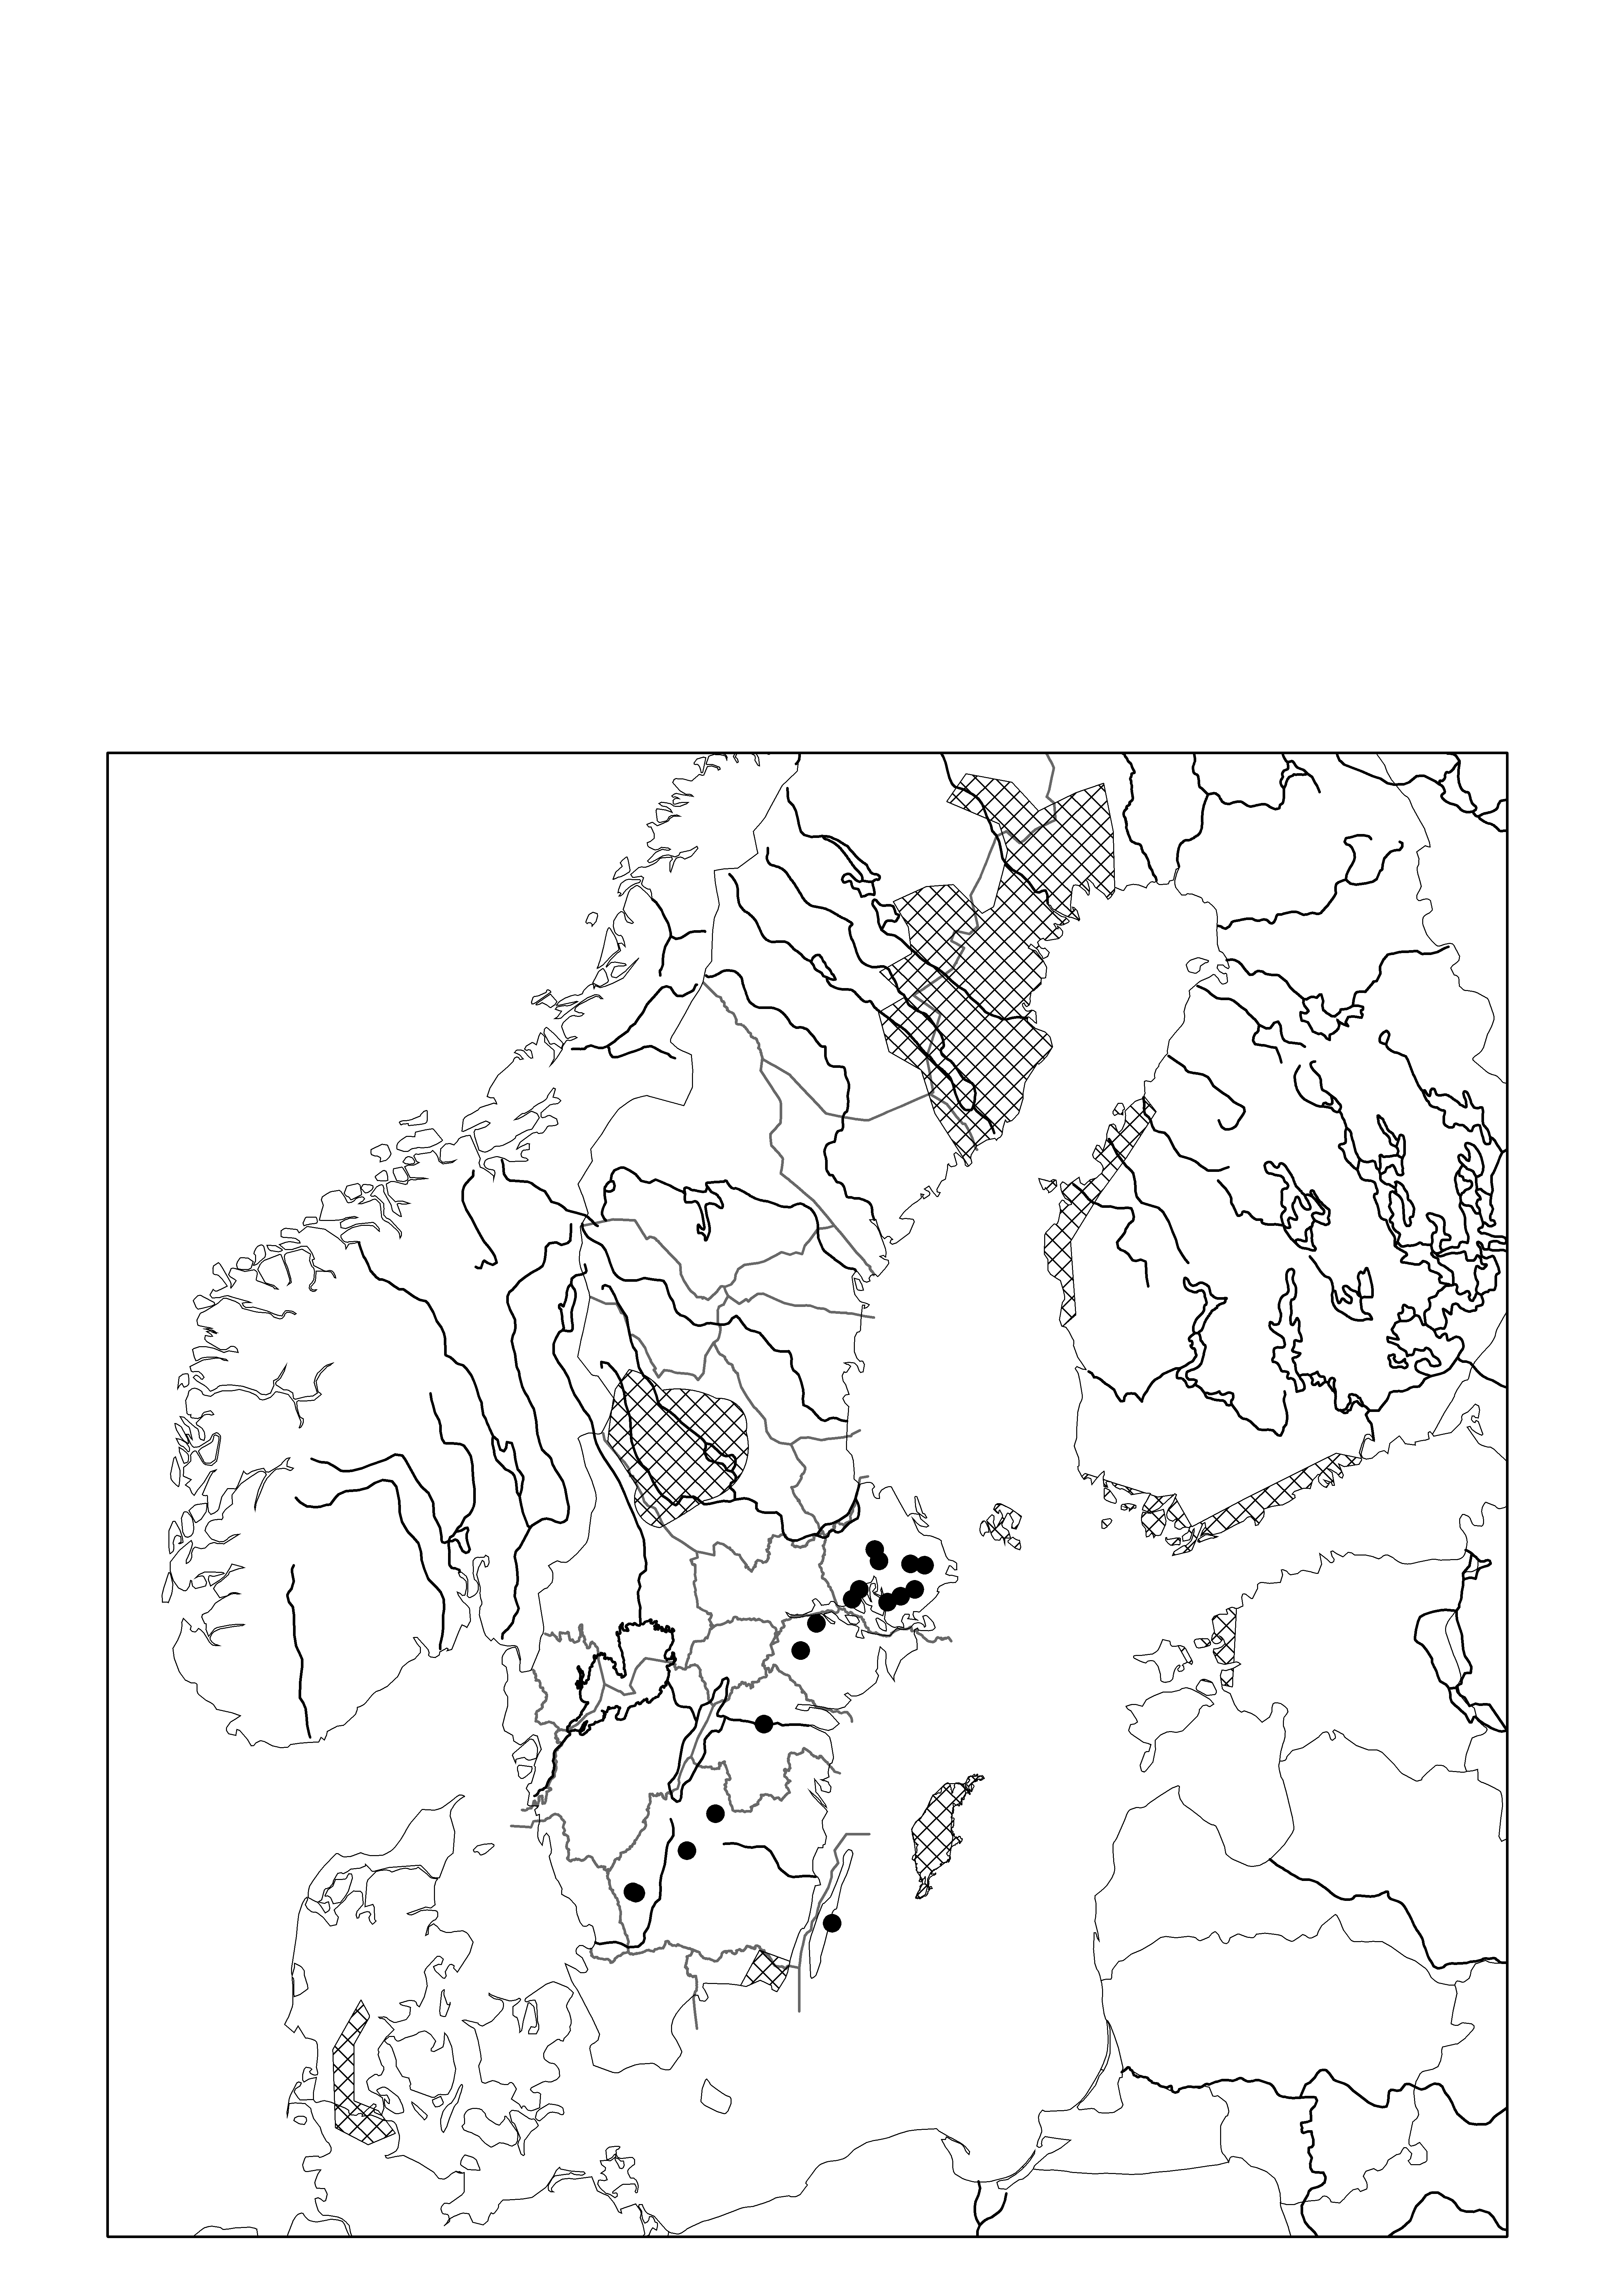
\includegraphics[height=.5\textheight]{figures/30_DistributionHjärJär}
\caption{The distribution of forms such as \textstyleLinguisticExample{hjär} and \textstyleLinguisticExample{jär} for ‘here’ according to Hesselman 1936. Crosshatched areas represent modern vernaculars, dots earlier attestations.}
\label{map:26}
\end{figure}

As Widmark points out, the sound change \textstyleLinguisticExample{\=e }{\textgreater} \textstyleLinguisticExample{ja }cannot have spread to the whole area at once, since there were no Swedish settlements in the northernmost part at that time, and the expansion of the Scandinavian-speaking population was not completed until several centuries later, in the the 13\textsuperscript{th} or 14\textsuperscript{th} centuries. The timetable is on the whole somewhat problematic. The spread of the Birka/Hedeby variety must have taken place quite early, in fact earlier than the spread of other changes that have been more general, such as the spread of definite marking. But what is notable in this context is the similarity between the distribution of the \textstyleLinguisticExample{jär }area and the other Peripheral Swedish phenomena discussed here, although \textstyleLinguisticExample{jär} is stronger in the south than many of the others. 

\section{Lexical innovations in the Peripheral Swedish area}

Among the numerous lexical items specific to Peripheral Swedish vernaculars, the most interesting ones in this context are those which are represented in different parts of the Peripheral Swedish area and which lack cognates both in older forms of Scandinavian and in modern Standard Swedish – that is, items which can be taken to be shared innovations in the Peripheral Swedish area. 

Given the old insight that each word has its own history, it is not easy to orient oneself in the geographical distribution of lexical items. What I shall point to here are a couple of high-frequency items that are fairly well represented in the Cat Corpus.

Words for ‘run’ appear to be relatively unstable in the sense that they are replaced frequently in languages. The most frequent word for ‘run’ in older forms of Scandinavian appears to have been \textstyleLinguisticExample{löpa }(or its cognates), but in modern Standard Swedish it has been replaced by \textstyleLinguisticExample{springa, }whose original meaning was ‘jump’. This development appears to be peculiar to Swedish and is not found in the other Scandinavian languages, nor has it extended to all non-standard varieties, as we shall now see. 

Words for ‘run’ occur on average about 10 times in the Cat stories, so there is relatively ample material for a comparison. There are two competitors to \textstyleLinguisticExample{springa, }which is the major alternative in about half the texts. One is \textstyleLinguisticExample{ränna}, which shows up in the two texts from Gotland (Fårömål also has \textstyleLinguisticExample{löpa} as a second choice).\footnote{ As can be seen from (), the verb \textit{renna} exists in Elfdalian, but may be used predominantly in the sense ‘to ski’.} The other one – \textstyleLinguisticExample{kuta} – is the most interesting from our point of view. The word exists also in Standard Swedish but the primary meaning indicated by older dictionaries is ‘walk with a stoop’. In colloquial language, on the other hand, it does mean ‘run’. \citet[371]{Hellquist1922} thinks that the two readings are derived by parallel but historically separate processes from the obsolete word \textstyleLinguisticExample{kut} ‘hump’. The reading ‘run’ is attested from the 16\textsuperscript{th} century, and in this sense the word is probably identical to the one found in the vernaculars. The distribution in the Cat Corpus (see \figref{map:27}) suggests that, as the major word for ‘run’, \textstyleLinguisticExample{kuta} is restricted to the Peripheral Swedish area, including Värmland. \textstyleLinguisticExample{Kute} ‘run’ exists in Norwegian dialects, but I have not been able to establish its distribution.

Another interesting item is the cognate set represented in Swedish by \textstyleLinguisticExample{häva} and found also in many other Germanic languages (e.g. English \textit{heave}) with the original meaning ‘lift, move upwards’. In Swedish vernaculars, it has expanded its meaning quite considerably. Thus, as far south as Småland, examples such as \textit{häva dom i grytan} ‘put them (the potatoes) in the pot’ are common according to the materials collected for the Swedish Dialect Dictionary. In the Peripheral Swedish area, cognates\textit{ }of \textit{häva} have developed into a general transitive verb of movement corresponding to English ‘put’, as exemplified by the following examples (they also show up in many lexicalized phrases):

\ea\label{}
\langinfo{Skellefteå country parish (NVb)}{}{}\\
\gll han  \textbf{ho} päninge  ni  plånboka\\
he  \textbf{put{\pst}} money.{\pl}.{\deff}  in  wallet.{\deff}\\
\glt ‘He put the money in the wallet’
\z

\ea\label{}
\langinfo{Norsjö (NVb)}{}{}\\
\gll ha  du  \textbf{het} på  de  vanta?\\
have.{\prs}  you  \textbf{put.{\supp}} on  you.{\obl}  mitten.{\deff}.{\pl}\\
\glt ‘Have you put mittens on?’
\z

\figref{map:27}shows the distribution of \textit{häva} cognates in the Cat Corpus. We see that the strongest area is Ovansiljan in Dalarna but that there are also strong points in southern Västerbotten and Ångermanland. 

\citet{Eaker1993} describes the distribution in Swedish vernaculars of the adjective \textit{grann} and some other adjectives related to it. In this connection, the most interesting case is \textstyleLinguisticExample{laggrann} ‘careful’, which is in modern vernaculars found in all of Norrland and Dalarna but may have also been used earlier in Västmanland and Uppland. 

 

\begin{figure}[h] 
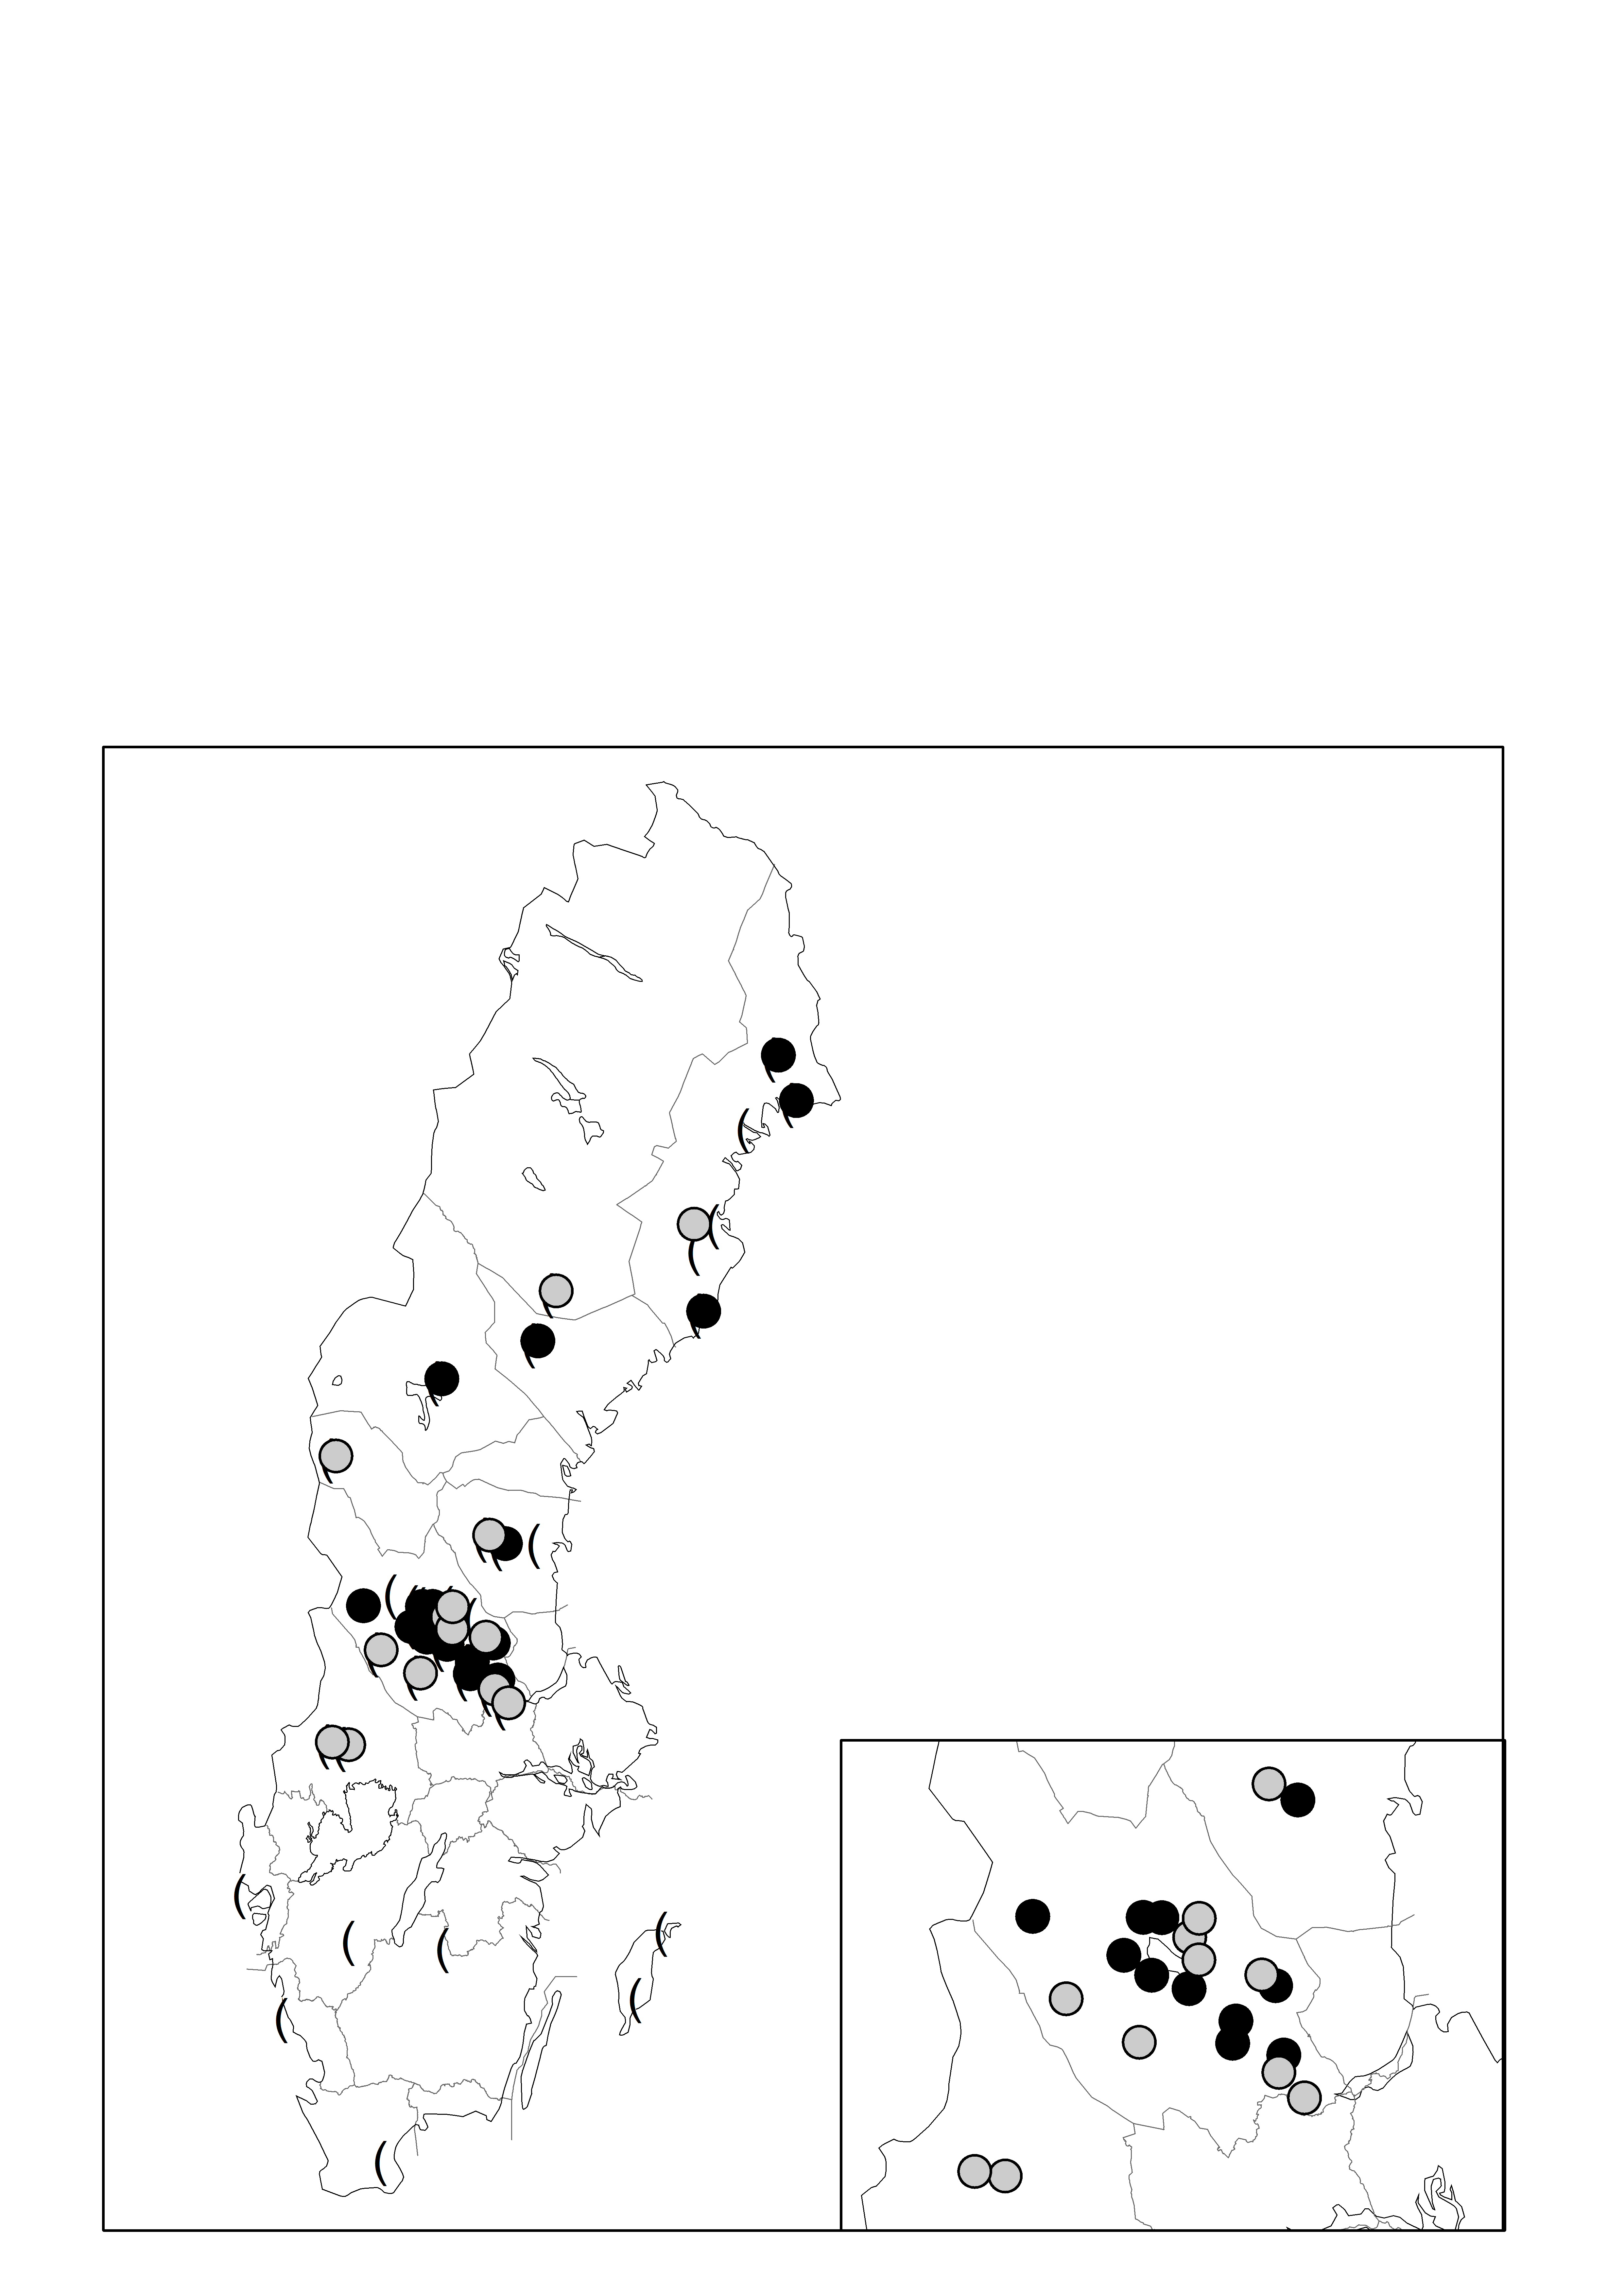
\includegraphics[height=.5\textheight]{figures/31_DistributionofKuta}
\caption{Distribution of \textit{kuta} ‘run’ in the Cat Corpus.}
\label{map:27}
\end{figure}

 

\begin{figure}[h] 
%\includegraphics[height=.5\textheight]{figures/32_DistributionofHäva}
\caption{Distribution of \textit{häva} ‘raise, put’ in the Cat Corpus}
\label{map:28}
\end{figure}

\subsection{Auxiliaries}

\citet{Holm1941} discusses the use of the verb \textstyleLinguisticExample{fara, }the original meaning of which is ‘travel’ or ‘go’, as an ingressive or future auxiliary. As an auxiliary with the meaning ‘begin’, \textstyleLinguisticExample{fara, }often in reduced forms such as \textstyleLinguisticExample{fa} or \textstyleLinguisticExample{fe}, is found in particular in the Northern Westrobothnian and the Ovansiljan areas, e.g. 

\ea\label{}
\langinfo{Lövånger (NVb)}{}{}\\
\gll Je  \textbf{for} no  väL  tröyt.\\
I  \textbf{start.{\pst}} {\prag}  become.{\inf}  tired\\
\glt ‘I started to become tired.’ (\citet[19]{Holm1942})
\z

\ea\label{}
\langinfo{Älvdalen (Os) }{}{}\\
\gll E  \textbf{fa} raingen.\\
it  \textbf{begin.{\prs}} rain.{\inf}\\
\glt ‘It’s beginning to rain.’ (\citet[115]{Levander1909})
\z

In Northern Västerbotten, there are also two other kinds of uses: the first one Holm characterizes as having a “futural meaning” (\citet[20]{Holm1941})

\ea\label{}
\langinfo{\label{bkm:Ref72064267}Lövånger (NVb)}{}{}\\
\gll He  kan  \textbf{fara} hall  op  inan  sönndan.\\
it  may.{\prs}  \textbf{begin.{\inf}} keep.{\inf}  up  before  Sunday.{\deff}\\
\glt  ‘It may stop raining before Sunday.’
\z

%\begin{styleTextkrper}
The second he labels “pleonastic” (\citet[21]{Holm1941}):

%\end{styleTextkrper}

\ea\label{}
\langinfo{Jörn (NVb)}{}{}\\
\gll Do  skul  pappen  \textbf{fara} ten  op  do.\\
then  shall.{\pst}  father.{\deff}  \textbf{begin.{\inf}} light  up  then\\
\glt ‘Then father was going to make a fire.’
\z

I am not certain if the last two groups of uses are really distinct from the first. The “futural” uses are not wholly convincing as such—they often involve some other modal marker such as \textstyleLinguisticExample{kan} ‘may’ in \REF{323}. It is not clear if similar examples can be found in Dalecarlian. 

Holm also quotes examples of \textstyleLinguisticExample{fara} as an auxiliary from Nyland, taken from \citet{Lundström1939}, such as

\ea\label{}
\langinfo{Pojo (Ny) }{}{}\\
\gll Ja  va  fj\={ɷ}jjo   år,  när  ja  \textbf{f\={ɷ}a} čän  b\={ɷ}äno   \\
I  be.{\pst}  fourteen  year.{\pl}  when  I  \textbf{go.{\pst}} serve.{\inf}  farmer.{\deff}  \\
\glt ‘I was fourteen, when I started working for the farmer.’ (\citet[133]{Lundström1939})
\z

The use in Nyland seems more restricted and may in Holm’s opinion represent a transitional stage, where the auxiliary keeps part of its original meaning. 

A similar use of \textstyleLinguisticExample{fara} is also found in Icelandic (both Old and Modern) and in certain Norwegian dialects. In these, however, an infinitive marker, or the preposition \textstyleLinguisticExample{til} ‘to’ followed by an infinitive marker, is used. 

Holm notes that there seem to be no examples of auxiliary uses of \textstyleLinguisticExample{fara} in older forms of Swedish which, he says, would be expected from the general distribution of these uses in time and space. Further research is needed, he says, and it would be premature to conclude that the auxiliary uses of \textstyleLinguisticExample{fara} have been distributed as a “contiguous whole” over the whole of Scandinavia.

\begin{figure}[h]

%\begin{styleBeschriftung}
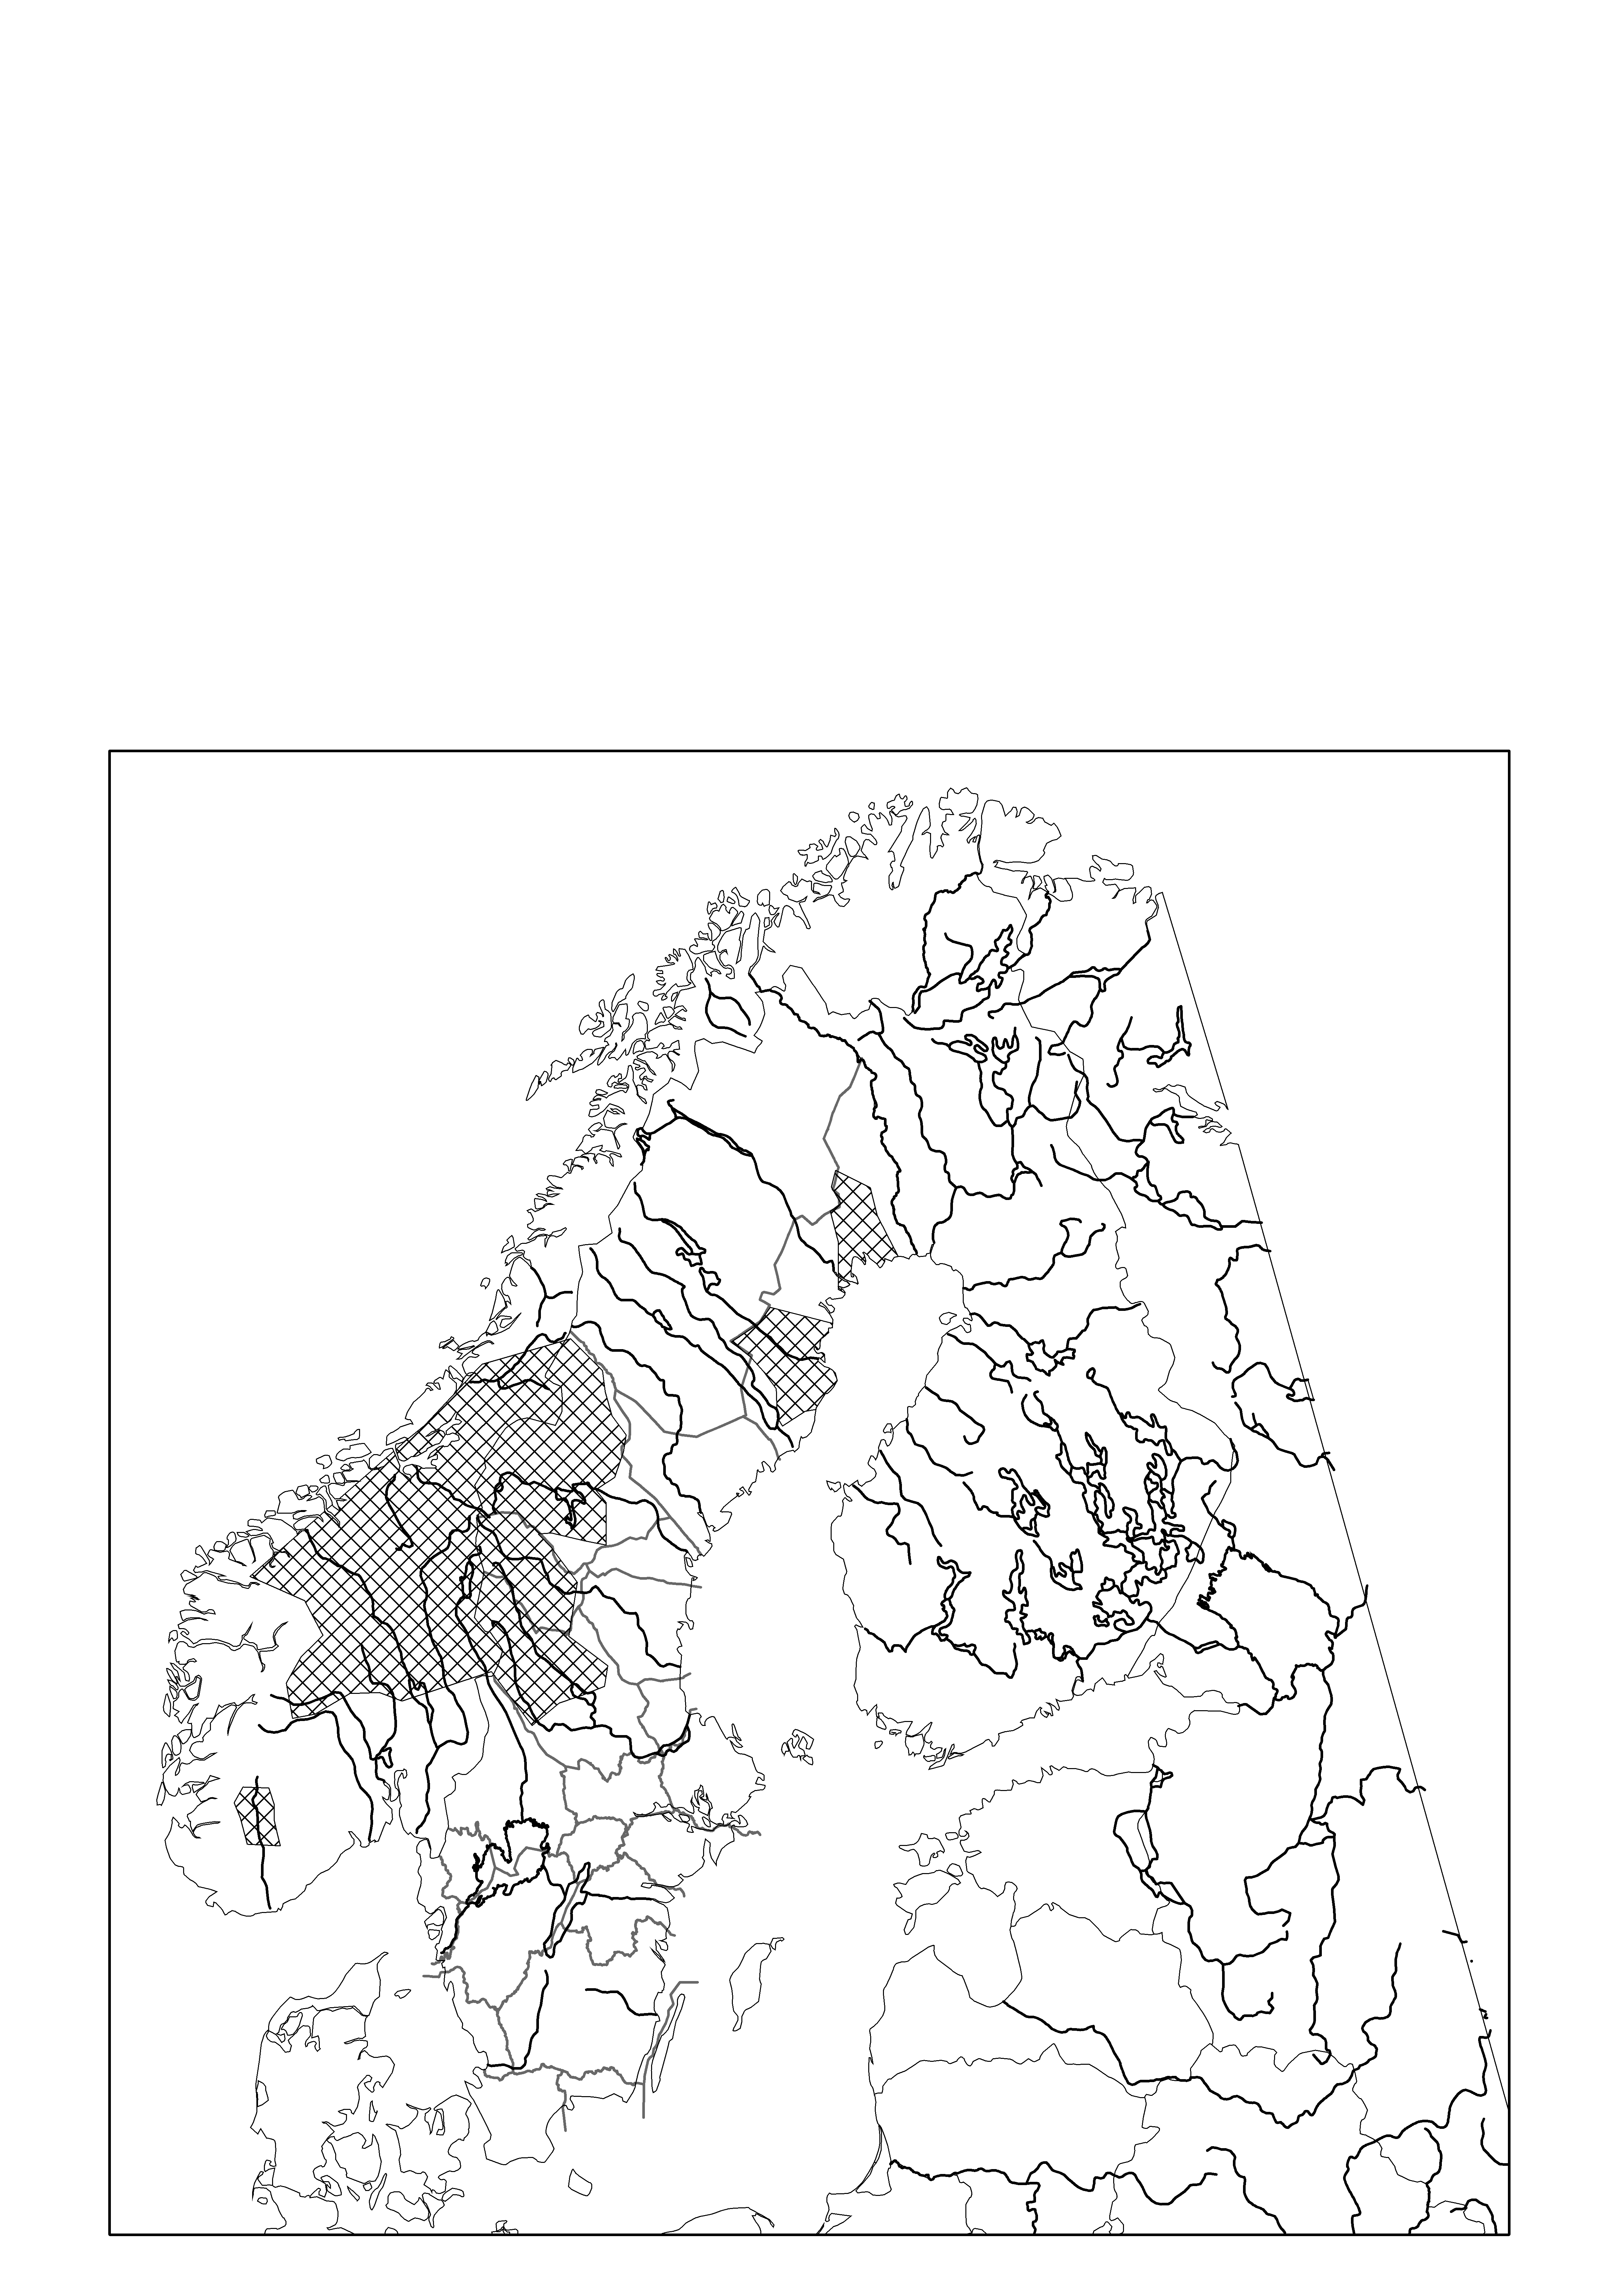
\includegraphics[height=.5\textheight]{figures/33_CoreAreasReinhammer}
\caption{Core areas of preserved dative use according to \citet{Reinhammar1973}.}
\label{map:29}

\end{figure}

\section{Conservative features of the Peripheral Swedish area}

Many of the conservative features of the Peripheral Swedish area are well-known and have been studied in detail. Most obviously, perhaps, is the retention of considerable parts of the morphology that were discarded in Central Scandinavian fairly early on.Thus, the old case system is at least partly preserved in several areas; this is particularly true for the dative case which is still alive in vernaculars in Dalarna, Härjedalen, Jämtland, Västerbotten and Norrbotten, with some remnants in Ångermanland and Medelpad (see \figref{map:29}). 

A three-way distinction between nominative, accusative, and dative is probably only found in the Ovansiljan area – the accusative case that has been claimed to exist in parts of Uppland is – or was – probably a general oblique case (\citet{DahlEtAl2006}). 

The vernaculars in Finland and Estonia do not feature the dative and accusative; one might perhaps think that the vicinity to Finnish and Estonian would favour the retainment of a complex case system. 

A three-gender system (rather than the two-gender system found in standard Danish and Swedish) has been generally preserved in the Peripheral Swedish vernaculars, but this is less significant, since it is true of most Peninsular Scandinavian vernaculars. 

In the pronoun system, one may note various forms of the 1\textsuperscript{st} person singular pronoun that contain the vowel \textstyleLinguisticExample{I, }such as \textstyleLinguisticExample{ik}, \textstyleLinguisticExample{ig}, \textstyleLinguisticExample{I}. It is somewhat unclear if this should be seen as a conservative feature or not – that is, whether the forms are derived directly from original “unbroken” forms such as Old Nordic \textstyleLinguisticExample{ek }or if they should be seen as reduced variants of “broken” forms like Standard Swedish \textstyleLinguisticExample{jag}. In any case, the \textstyleLinguisticExample{i}{}-forms are found, characteristically, in Norrbotten (although apparently restricted to Överkalix (Kx) in the north), most of Westrobothnian, all of Ovansiljan, and Malung (Vd). 

In verbal morphology, subject agreement is retained in Dalecarlian, in particular the Ovansiljan area, Northern Westrobothnian, and Norrbothnian. The distinction between singular and plural subjects is most widely marked but in Dalarna there is also special marking of the 1\textsuperscript{st} and 2\textsuperscript{nd} persons in the plural. It should be mentioned that verbs are also inflected for person and number in an area in Götaland (parts of Västergötland, Halland, and Småland) and in Gotland, Finland and parts of Estonia.

In phonology, the old \textstyleLinguisticExample{w}, corresponding to Central Scandinavian \textstyleLinguisticExample{v}, is retained, either only after consonants (including \textstyleLinguisticExample{h}, which later disappeared before \textstyleLinguisticExample{w/v}) or more generally in word-initial position (mainly Ovansiljan). Again, the same situation also obtains in parts of Götaland – much the same area as the one mentioned in the preceding paragraph but also including parts of Bohuslän. In another phonological development, Old Nordic \textstyleLinguisticExample{\=e} became \textstyleLinguisticExample{ä }in large parts of southern Scandinavia, but is retained in Norway, northern Bohuslän, northern Dalsland, Dalecarlian, Norrlandic and in the Trans-Baltic area (\citet[57]{Wessén1966}).

There are also a number of conservative syntactic features, some of which have not been properly described in the literature. I shall discuss two of them in the following sections.

\subsection{Infinitive constructions}
\label{sec:6.4.1}

Swedish employs an “infinitive marker” \textstyleLinguisticExample{att}, commonly pronounced [ɔ], which corresponds fairly well to English \textstyleLinguisticExample{to }with respect to its distribution. It is homographic to the complementizer \textstyleLinguisticExample{att} ‘that’ but in spoken language it is usually distinct from the latter, which is never reduced phonetically. Instead, the infinitive marker is homophonous with the reduced form of the conjunction \textstyleLinguisticExample{och} [ɔ], with which it is frequently confused. The two \textstyleLinguisticExample{att} also differ etymologically: the complementizer is considered to derive from the demonstrative pronoun \textstyleLinguisticExample{þat}, whereas the infinitive marker comes from the preposition \textstyleLinguisticExample{at} ‘to’ (cf. \sectref{sec:5.6}) and was first used in final constructions: 

\ea\label{}
\langinfo{Early Written Medieval Swedish}{}{}\\
\gll Han  är  i  sokn  farin,  siukum  \textbf{at} \textbf{hialpä.}\\
he  be.{\prs}  in  parish  go.PP  sick.{\dat}.{\pl}  \textbf{{{\inf}m}} \textbf{help.{\inf}}\\
\glt ‘He has gone to the parish to help the sick.’ (Older Västgöta Law, \citet[136]{Wessén1956}) 
\z

In older forms of Swedish, the infinitive marker had a more restricted use than in Modern Swedish. In particular, we find bare infinitives as complements of adjectives as in:

\ea\label{}
\langinfo{Early Written Medieval Swedish}{}{}\\
\gll Bätra  är  dyrt  köpa  än  swälta.  \\
better  be.{\prs}  dearly  buy.{\inf}  than  starve.{\inf}  \\
\glt ‘It is better to buy dearly than to starve.’ (\citet[138]{Wessén1956})
\z

Wessén notes that in “Older Modern Swedish” the preposition \textstyleLinguisticExample{till} ‘to’ was frequently used as an infinitive marker. In fact, judging from the Cat Corpus material, cognates of this preposition are used very widely in vernaculars over most of Sweden (the old Danish provinces being an exception), and are in many cases the primary choice for an infinitive marker. The impression one gets is that \textstyleLinguisticExample{att, }when it does occur, is due to influence from the standard language. 

In addition, a few conservative vernaculars seem to retain the older pattern where the infinitive marker is used more sparingly. Compare the following adjective complement uses of infinitives from the Cat Corpus:

\ea\label{}
\langinfo{Älvdalen (Os)}{}{}\\
\gll E  war  do  fanta  me  it  so  litt\\
it  be.{\pst}  then  devil\_take  me  {\neg}  so  easy\\
\gll \textbf{bigrip} \textbf{sig} o  kellinger,  itsä!\\
\textbf{understand.{\inf}} \textbf{{\refl}} on  woman.{\pl}  {\neg}\\
\glt  ‘It wasn’t easy, damn it, to understand women!’ (Cat Corpus)
\z

\ea\label{}
\langinfo{Nås (Vd)}{}{}\\
\gll Hä  va  då  innt  lätt  \textbf{begri´p} \textbf{sä} på  kvinnfôƚƚk  innt!\\
it  be.{\pst}  then  {\neg}  easy  \textbf{understand.{\inf}} \textbf{{\refl}} on  woman.{\pl}  {\neg}\\
\glt ‘It really wasn’t easy to understand women!’ (Cat Corpus)
\z

\ea\label{}
\langinfo{\textit{Skelletmål} (NVb)}{}{}\\
\gll Hä  jer  väl  bäst  \textbf{pass} \textbf{sä.}\\
it  be.{\prs}  {\prag}  best  \textbf{look\_out.{\inf}} \textbf{{\refl}}\\
\glt ‘One had better look out.’ (Cat Corpus)
\z

\ea\label{}
\langinfo{Sävar (SVb)}{}{}\\
\gll Hä  tö  fäll  va  bäst  \textbf{akt}\textbf{  sä.}\\
it  ought\_to  {\prag}  be.{\inf}  best  \textbf{be\_careful\_about.{\inf}} \textbf{{\refl}}\\
\glt ‘One had probably better look out.’ (Cat Corpus)
\z

These examples come from Dalecarlian and Northern Westrobothnian, the two most conservative regions in the Peripheral Swedish area. But \citet[99]{KällskogEtAl1993} also quote examples from Roslagen along the coast of Uppland, in slightly different syntactic contexts:

\ea\label{}
\langinfo{Väddö (Up)}{}{}\\
\gll de  håller  \textbf{spara}\\
it  keep.{\prs}  \textbf{save.{\inf}}\\
\glt ‘it will keep if you save it [lit. it keeps to save]’
\z

\ea\label{}
\langinfo{Hållnäs (Up)}{}{}\\
\gll å  då  va  de  \textbf{fåljâs} åot\\
and  then  be.{\pst}  it  \textbf{follow\_each\_other.{\inf}} at\\
\glt ‘and then they had to go together’ 
\z

In other words, infinitive constructions are interesting in two ways: (i) the choice of infinitive marker is one feature where modern Standard Swedish differs from most vernaculars spoken in historical Sweden but is similar to Standard Danish and the vernaculars of the previous Danish provinces; (ii) the more restricted use of infinitive markers in general is still another conservative feature common to Dalarna and Västerbotten, extending also to Uppland. 

\subsection{Temporal subjunctions}

\citet{Vallmark1937} studied the distribution of temporal subjunctions in the Swedish dialect area. In modern spoken Standard Swedish the dominant translation of English \textstyleLinguisticExample{when} is \textstyleLinguisticExample{när}, which is also used as an interrogative adverb. A more formal or bookish alternative is \textstyleLinguisticExample{då}, whose major sense is ‘then’, and which is attested from Runic Swedish, where it appears to have been the primary choice. \textstyleLinguisticExample{När }started to be used as a subjunction in Written Medieval Swedish but was still relatively rare there. Its subsequent spread has not been complete: many conservative vernaculars lack it, or still use \textstyleLinguisticExample{då }as a natural alternative. Elfdalian goes its own way: \textstyleLinguisticExample{mes} (etymologically identical to Swedish \textstyleLinguisticExample{medan(s)} ‘while’) is used for singular events or periods in the past, \textstyleLinguisticExample{da(r)} (etymologically ‘there’) is used in other cases (Å\citet[152]{Åkerberg2012}). The Cat Corpus material on the whole confirms the picture given by Vallmark. Areas that retain \textstyleLinguisticExample{då} thus include the Dalecarlian area except Älvdalen; Norrland except southern Hälsingland, Gästrikland, most of Jämtland, \textit{Pitemål} and \textit{Nederkalixmål}; Ostrobothnia, Åboland and Nyland; Estonia; and northern Gotland (see \figref{map:30}). In Danish and Norwegian, \textstyleLinguisticExample{da} (etymologically the same as Swedish \textstyleLinguisticExample{då}) and \textstyleLinguisticExample{når} have a division of labour which resembles that between \textstyleLinguisticExample{als} and \textstyleLinguisticExample{wenn} in German. 

A similar story can be told about the verbs for ‘become’ (\citet{Markey1969}). In the late Middle Ages, the verb \textstyleLinguisticExample{bliva }(in Modern Swedish usually \textstyleLinguisticExample{bli}), with the original meaning ‘remain’ and emanating from Low German \textstyleLinguisticExample{blîwen}, started to take over the domain of the verb \textstyleLinguisticExample{varda} ‘become’ in Scandinavian. Again, the victory was only partial. While \textstyleLinguisticExample{bli }appears to reign supreme in most of Götaland (including Gotland), southern Finland and Estonia, even colloquial Standard Swedish as spoken in the Mälar provinces retains the alternative past tense form \textstyleLinguisticExample{vart} ‘became’ of \textstyleLinguisticExample{varda}, although all the other forms have disappeared. Most vernaculars of Svealand and Norrland also retain the supine form \textstyleLinguisticExample{vurti} (or similar). In some areas, however, the whole paradigm still exists (see \figref{map:32}), including large parts of Ovansiljan, Västerdalarna, Jämtland, Ångermanland, Västerbotten, Norrbotten, and Ostrobothnia.

The vernaculars of the Peripheral Swedish area preserve many lexical items that have been discarded in Standard Swedish. As an example of an item with a wide distribution, descendants of Old Swedish \textstyleLinguisticExample{fæghin }‘happy’ (cognate of English \textstyleLinguisticExample{fain}) may be mentioned as the standard counterpart of Swedish \textstyleLinguisticExample{glad}, e.g. Älvdalen \textstyleLinguisticExample{faingin}, Skellefteå \textstyleLinguisticExample{fajjen}, Färila \textstyleLinguisticExample{fäjjen}. (See \figref{map:32}.) What is less conspicuous are cases where some Swedish lexical item is missing from a vernacular and replaced by a synonymous word that also exists in Swedish. Consider the words for ‘find’ in Swedish. While \textstyleLinguisticExample{finna }is still quite viable in written Swedish, the natural alternative in most spoken varieties is \textstyleLinguisticExample{hitta}. Both these words were found with the same meaning in Written Medieval Swedish, although \textstyleLinguisticExample{finna} may reasonably be assumed to be the older word, with cognates in all branches of Germanic. Most pertinent to our context, we find \textstyleLinguisticExample{hitta} in the preface to the Upplandic Law:

\ea\label{}
\langinfo{Early Written Medieval Swedish}{}{}\\
\gll Hwat  ær  wi  \textbf{hittum} i  hans  laghsaghu\\
what  ever  we  \textbf{find.{\prs}.1{\pl}} in  his  law.{\dat}\\
\gll ær  allum  mannum\\
that  all.{\dat}.{\pl}  man.{\dat}.{\pl}\\
\gll þarfflikt  ær  þæt  sætium  wir  i  bok  þæssæ.\\
useful  be.{\prs}  that  put.{\prs}.1{\pl}  we  in  book  this.{\f}.{\acc}\\
\glt ‘Whatever we find in his law that is useful for everyone we include in this book.’
\z

Turning now to the Cat Corpus, the Swedish version of the text contains three occurrences of the word \textstyleLinguisticExample{hitta} but none of \textstyleLinguisticExample{finna}, which is natural given the colloquial nature of the story. When checking how these are rendered in the other versions, we can see a widespread reluctance in the vernaculars to use the word \textstyleLinguisticExample{hitta}. At least nine versions use \textstyleLinguisticExample{finna} consistently, and about ten more do so in one or two cases of the three relevant ones. Except for Sotenäs (Bo), all these versions emanate from the northern side of \textstyleLinguisticExample{limes norrlandicus}, and among the more consistent cases we find, not unexpectedly, Älvdalen (Os) and the texts from the Northern Westrobothnian and Norrbothnian areas. In many of these texts, however, \textstyleLinguisticExample{hitta} shows up combined with the counterpart of the preposition \textstyleLinguisticExample{på} ‘on’ in the meaning ‘to think of, make up’:

\ea\label{}
\langinfo{Älvdalen (Os)}{}{}\\
\gll Wen  al  ig  itt  o  {i dag},  truä?\\
what  shall.{\prs}  I  find.{\inf}  on  today  think.{\inf}\\
\glt ‘What shall I think of today, I wonder.’
\z

It thus seems that \textstyleLinguisticExample{hitta} in its major use has never made its way into a significant number of Peripheral Swedish varieties. The natural conclusion would be that \textstyleLinguisticExample{hitta} was not part of the variety of Scandinavian which is the common ancestor of those varieties. In at least this respect, then, that language would differ from that of the Upplandic law. 

\begin{figure}[h]
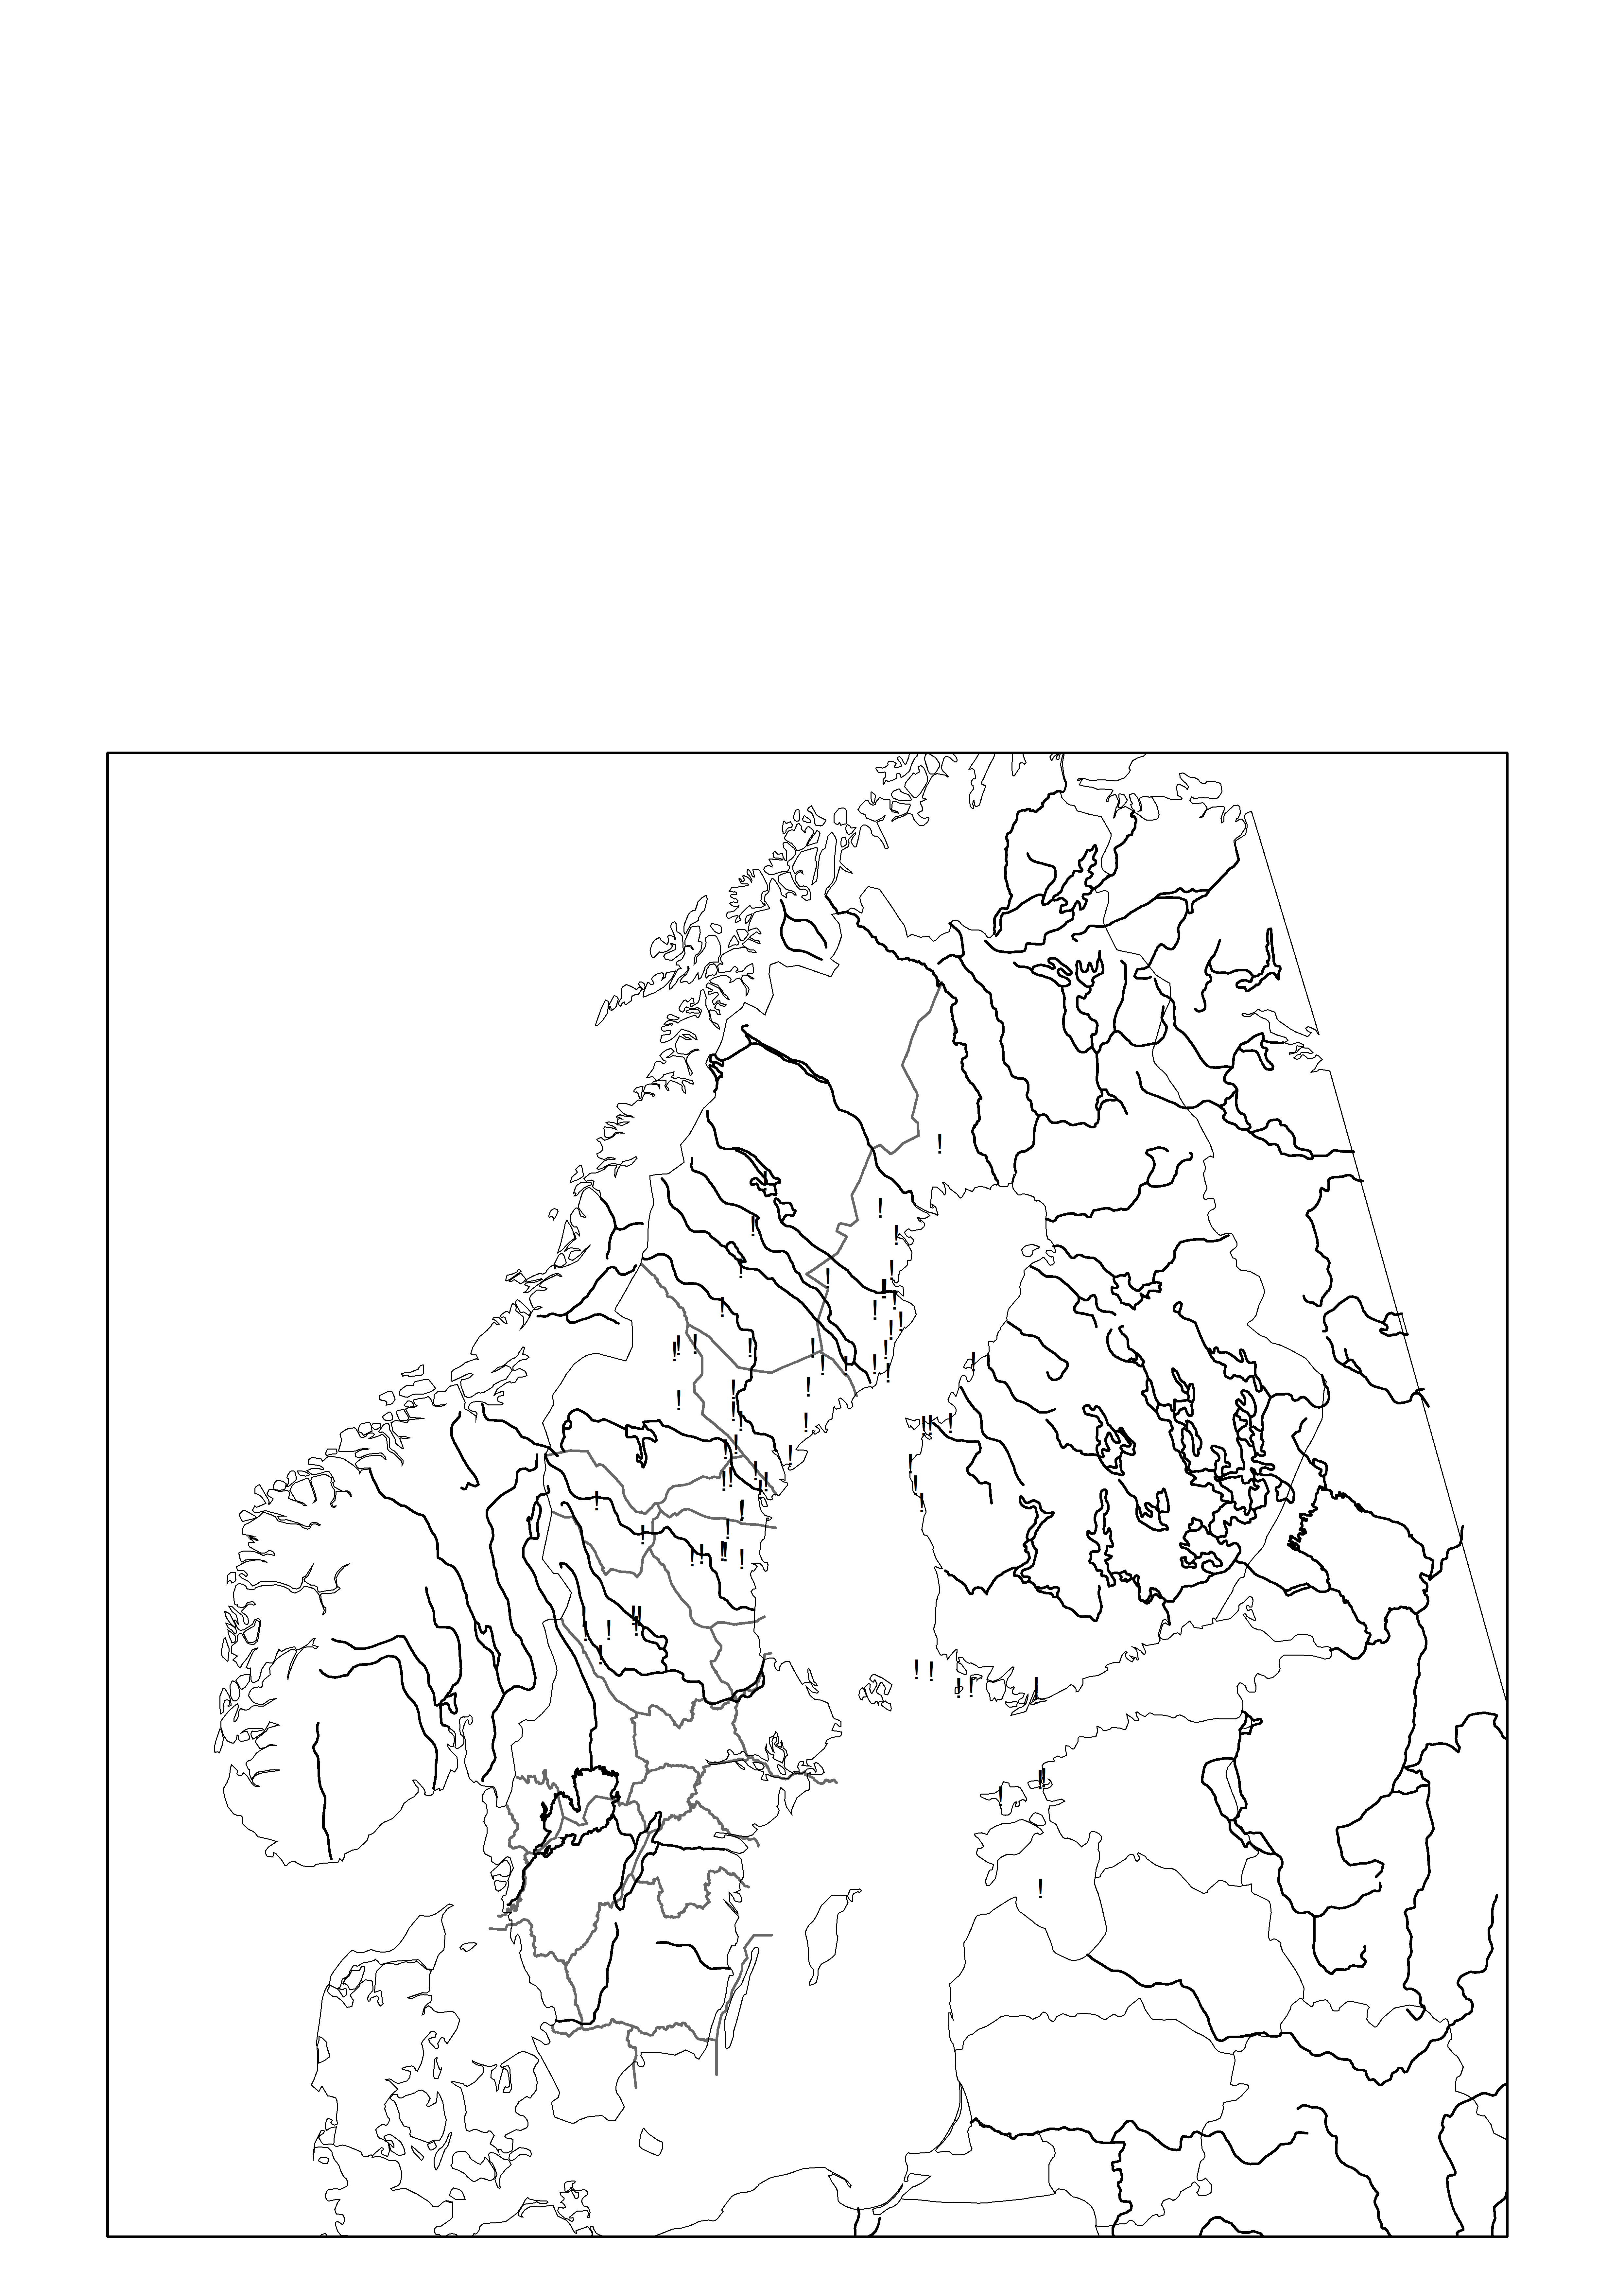
\includegraphics[height=.5\textheight]{figures/34_CoreAreasVallmark}
\caption{Vernaculars with predominant \textstyleLinguisticExample{då }as temporal subjunction according to \citet{Vallmark1937}.  }
\label{map:30}
\end{figure}

\begin{figure}[h]
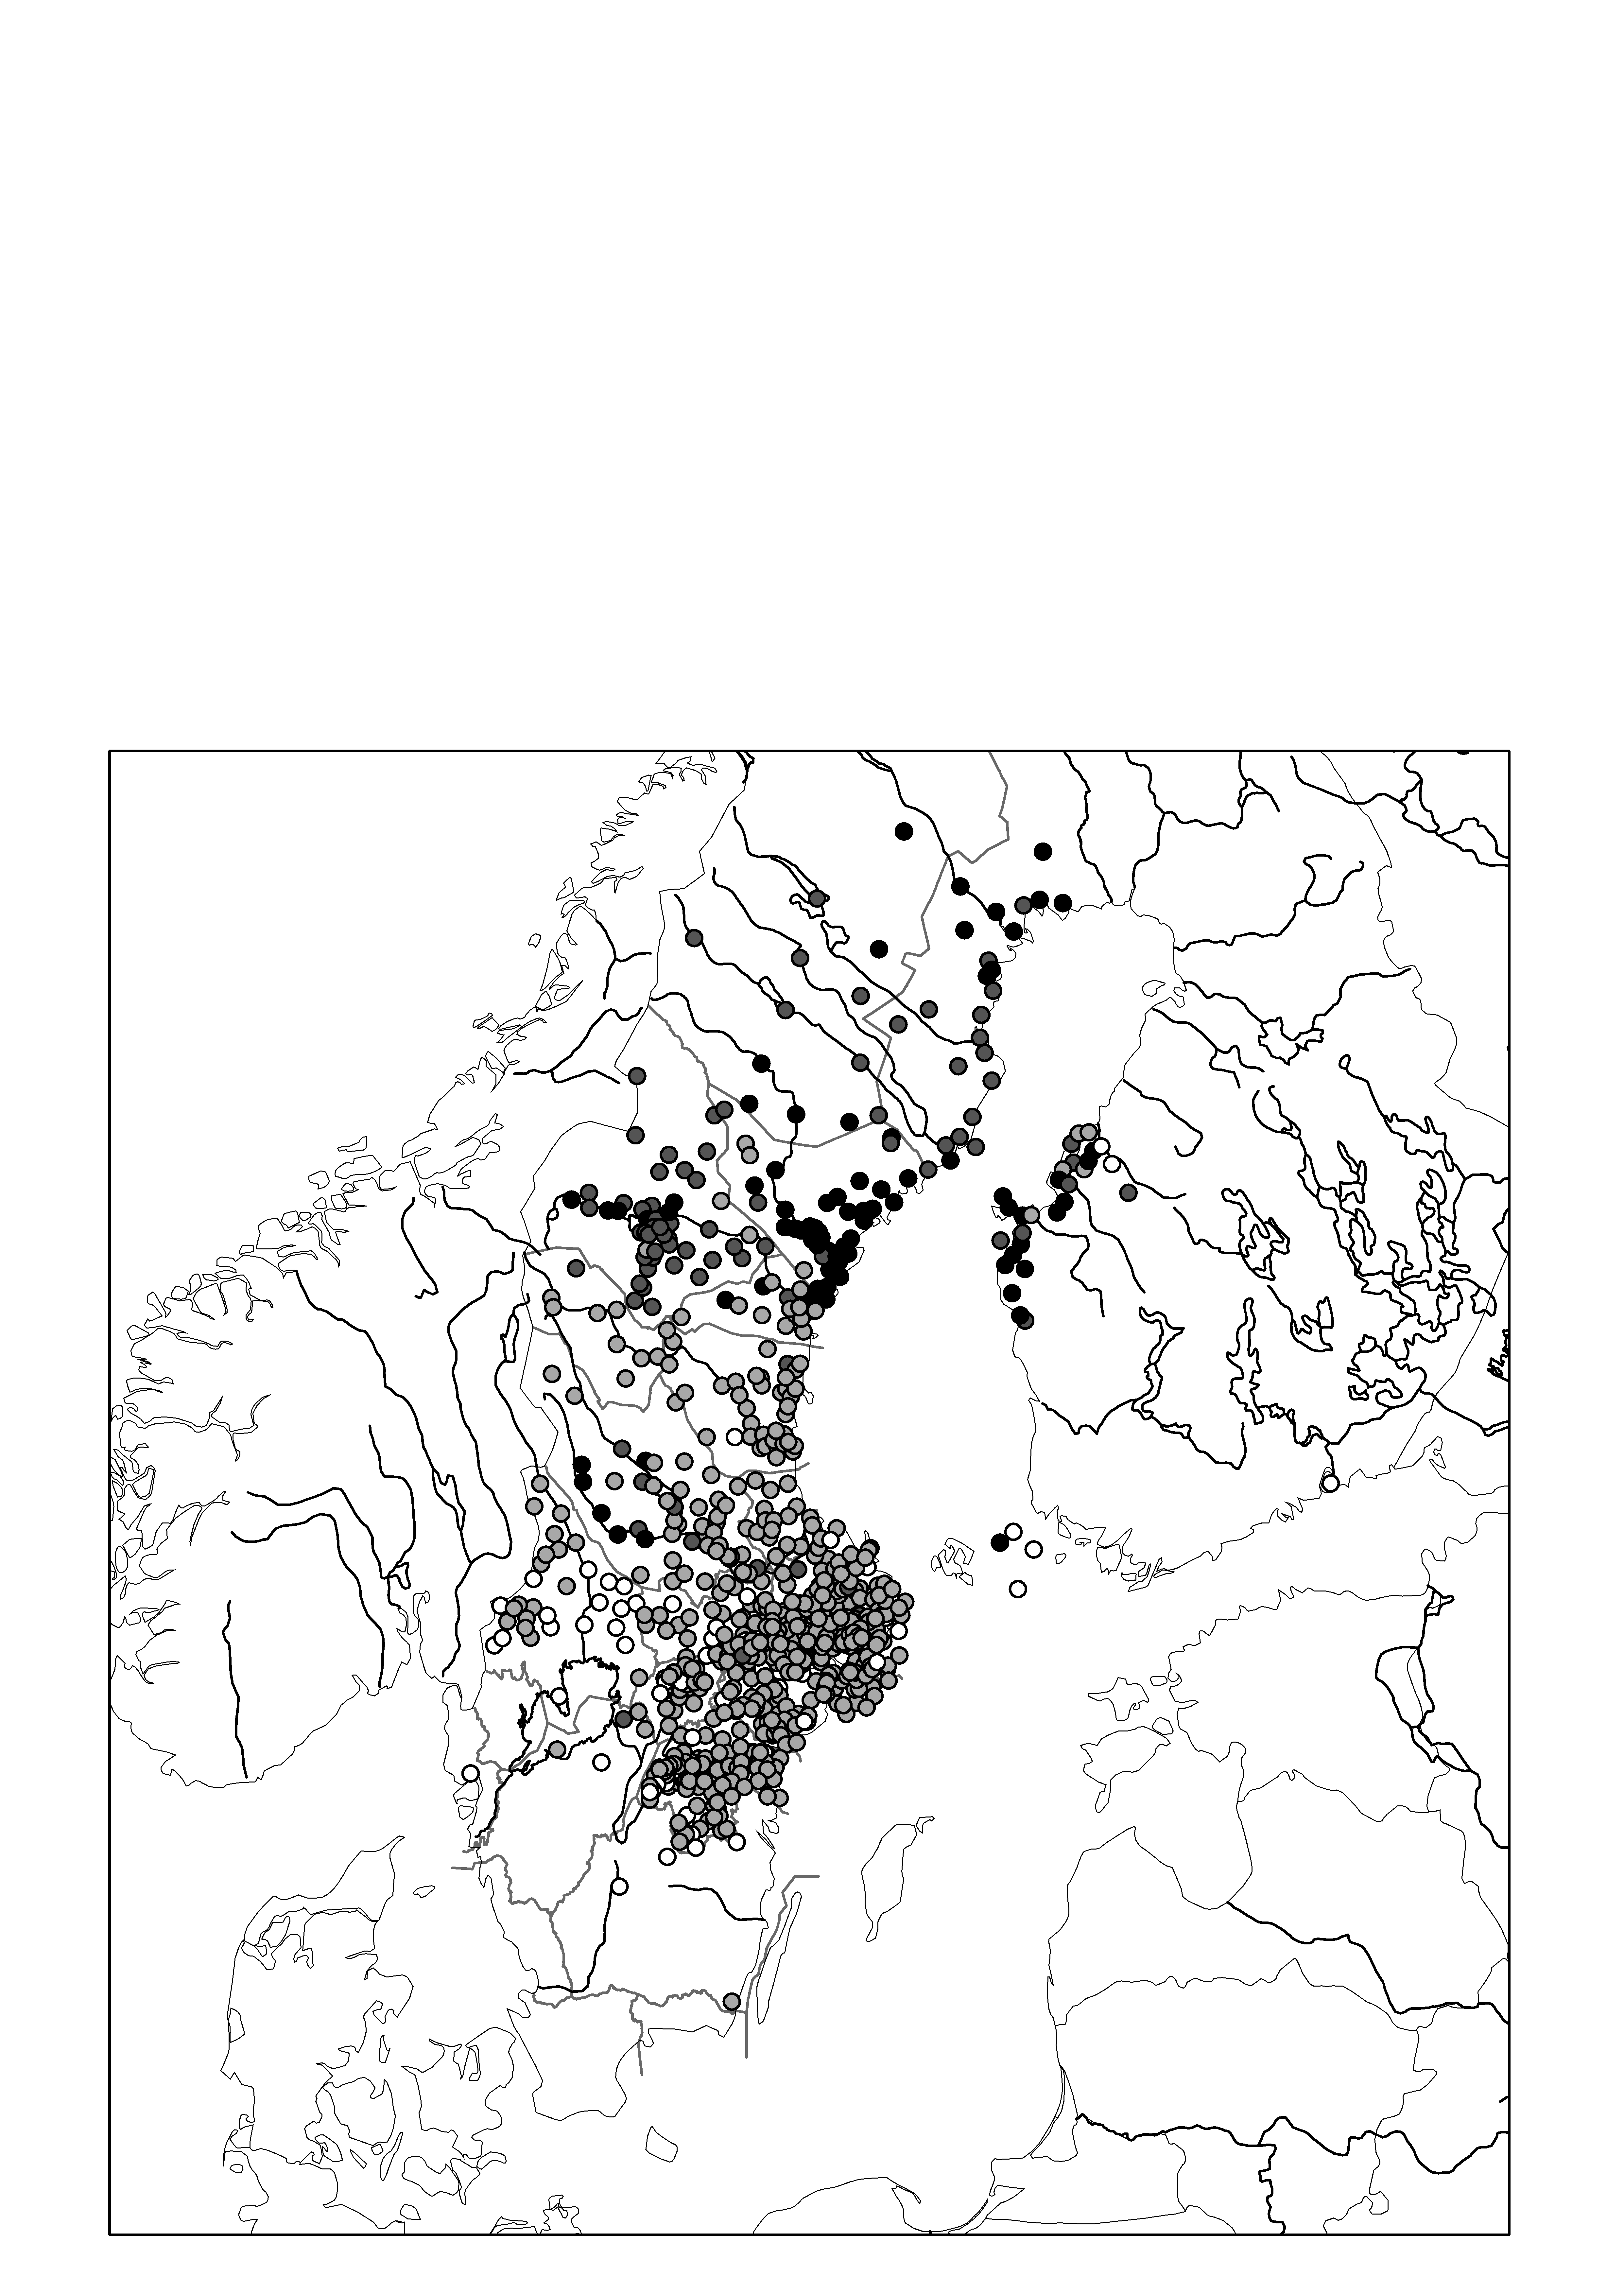
\includegraphics[height=.5\textheight]{figures/35_RetainmentofVarda}
\caption{Degree of retainment of \textstyleLinguisticExample{varda} paradigm in the Swedish dialect area (\citet{Markey1969}). Black circles – full paradigm retained; grey circles – at least two forms retained; white circles – past tense only. }
\label{map:31}
\end{figure}


\begin{figure}[h]
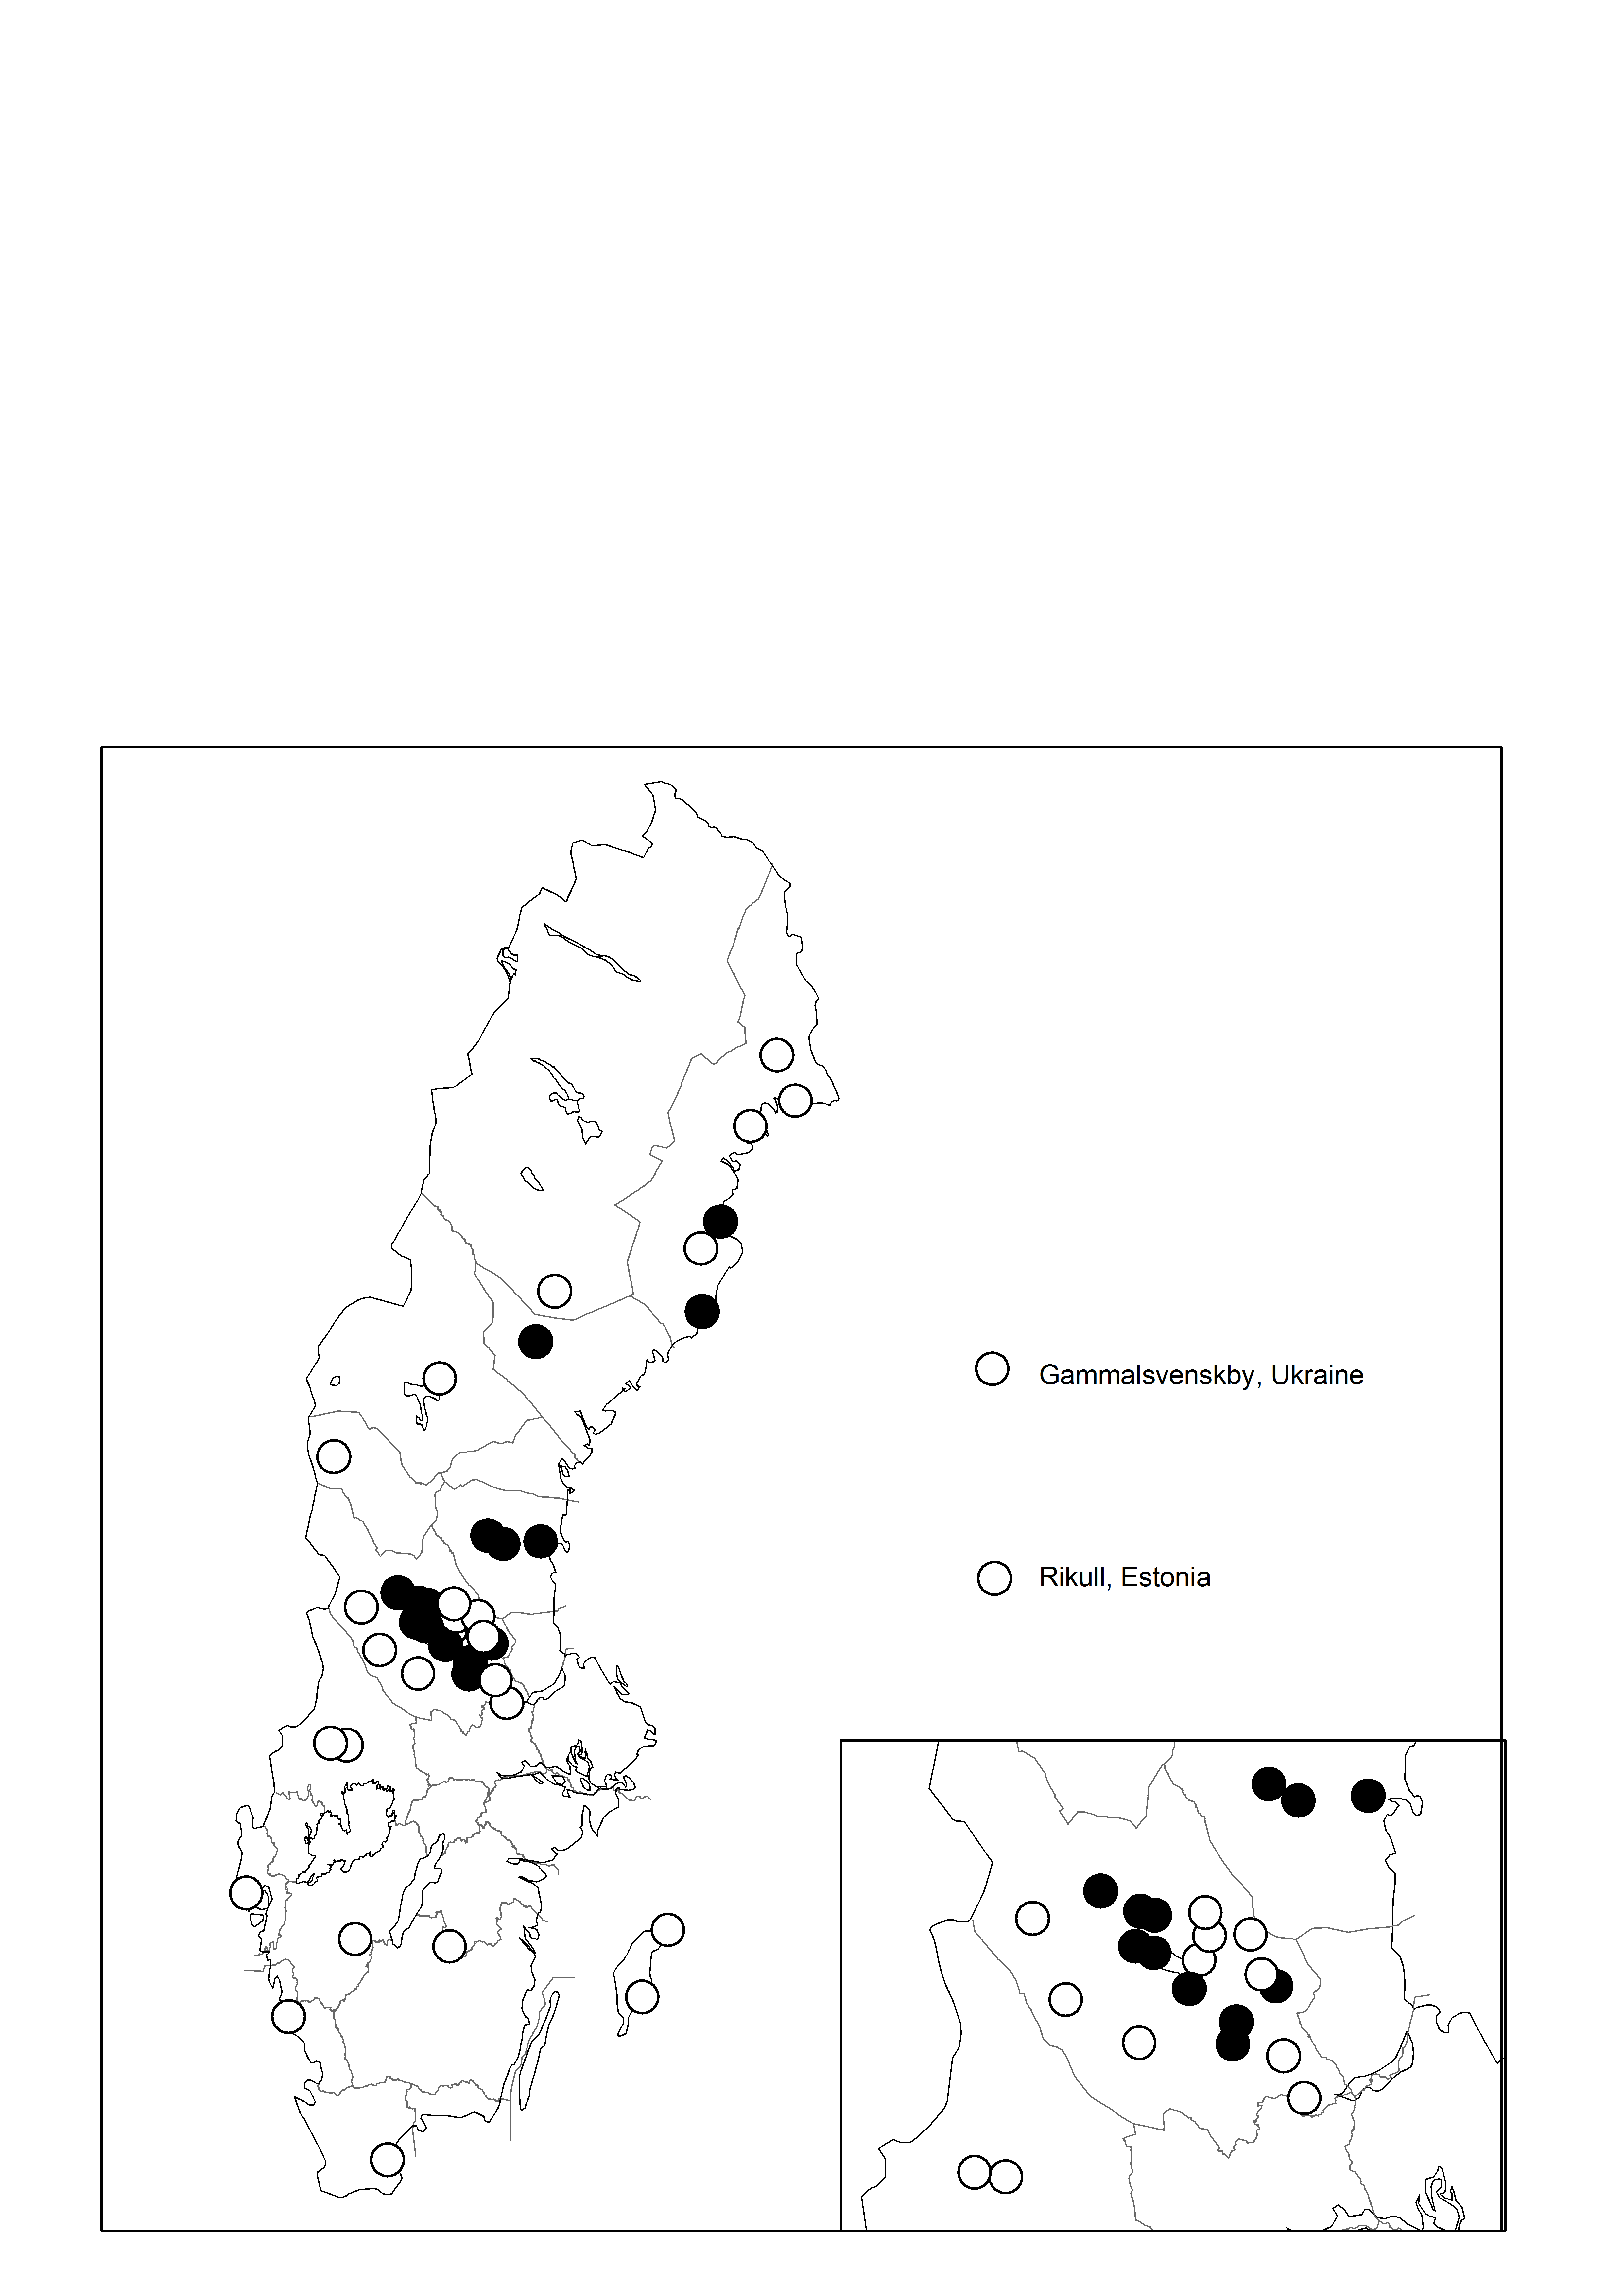
\includegraphics[height=.5\textheight]{figures/36_CognatesCatCorpus}
\caption{Cognates of \textstyleLinguisticExample{fæghin} in the Cat Corpus (filled circles).}
\label{map:32}
\end{figure}

\begin{figure}[h]
%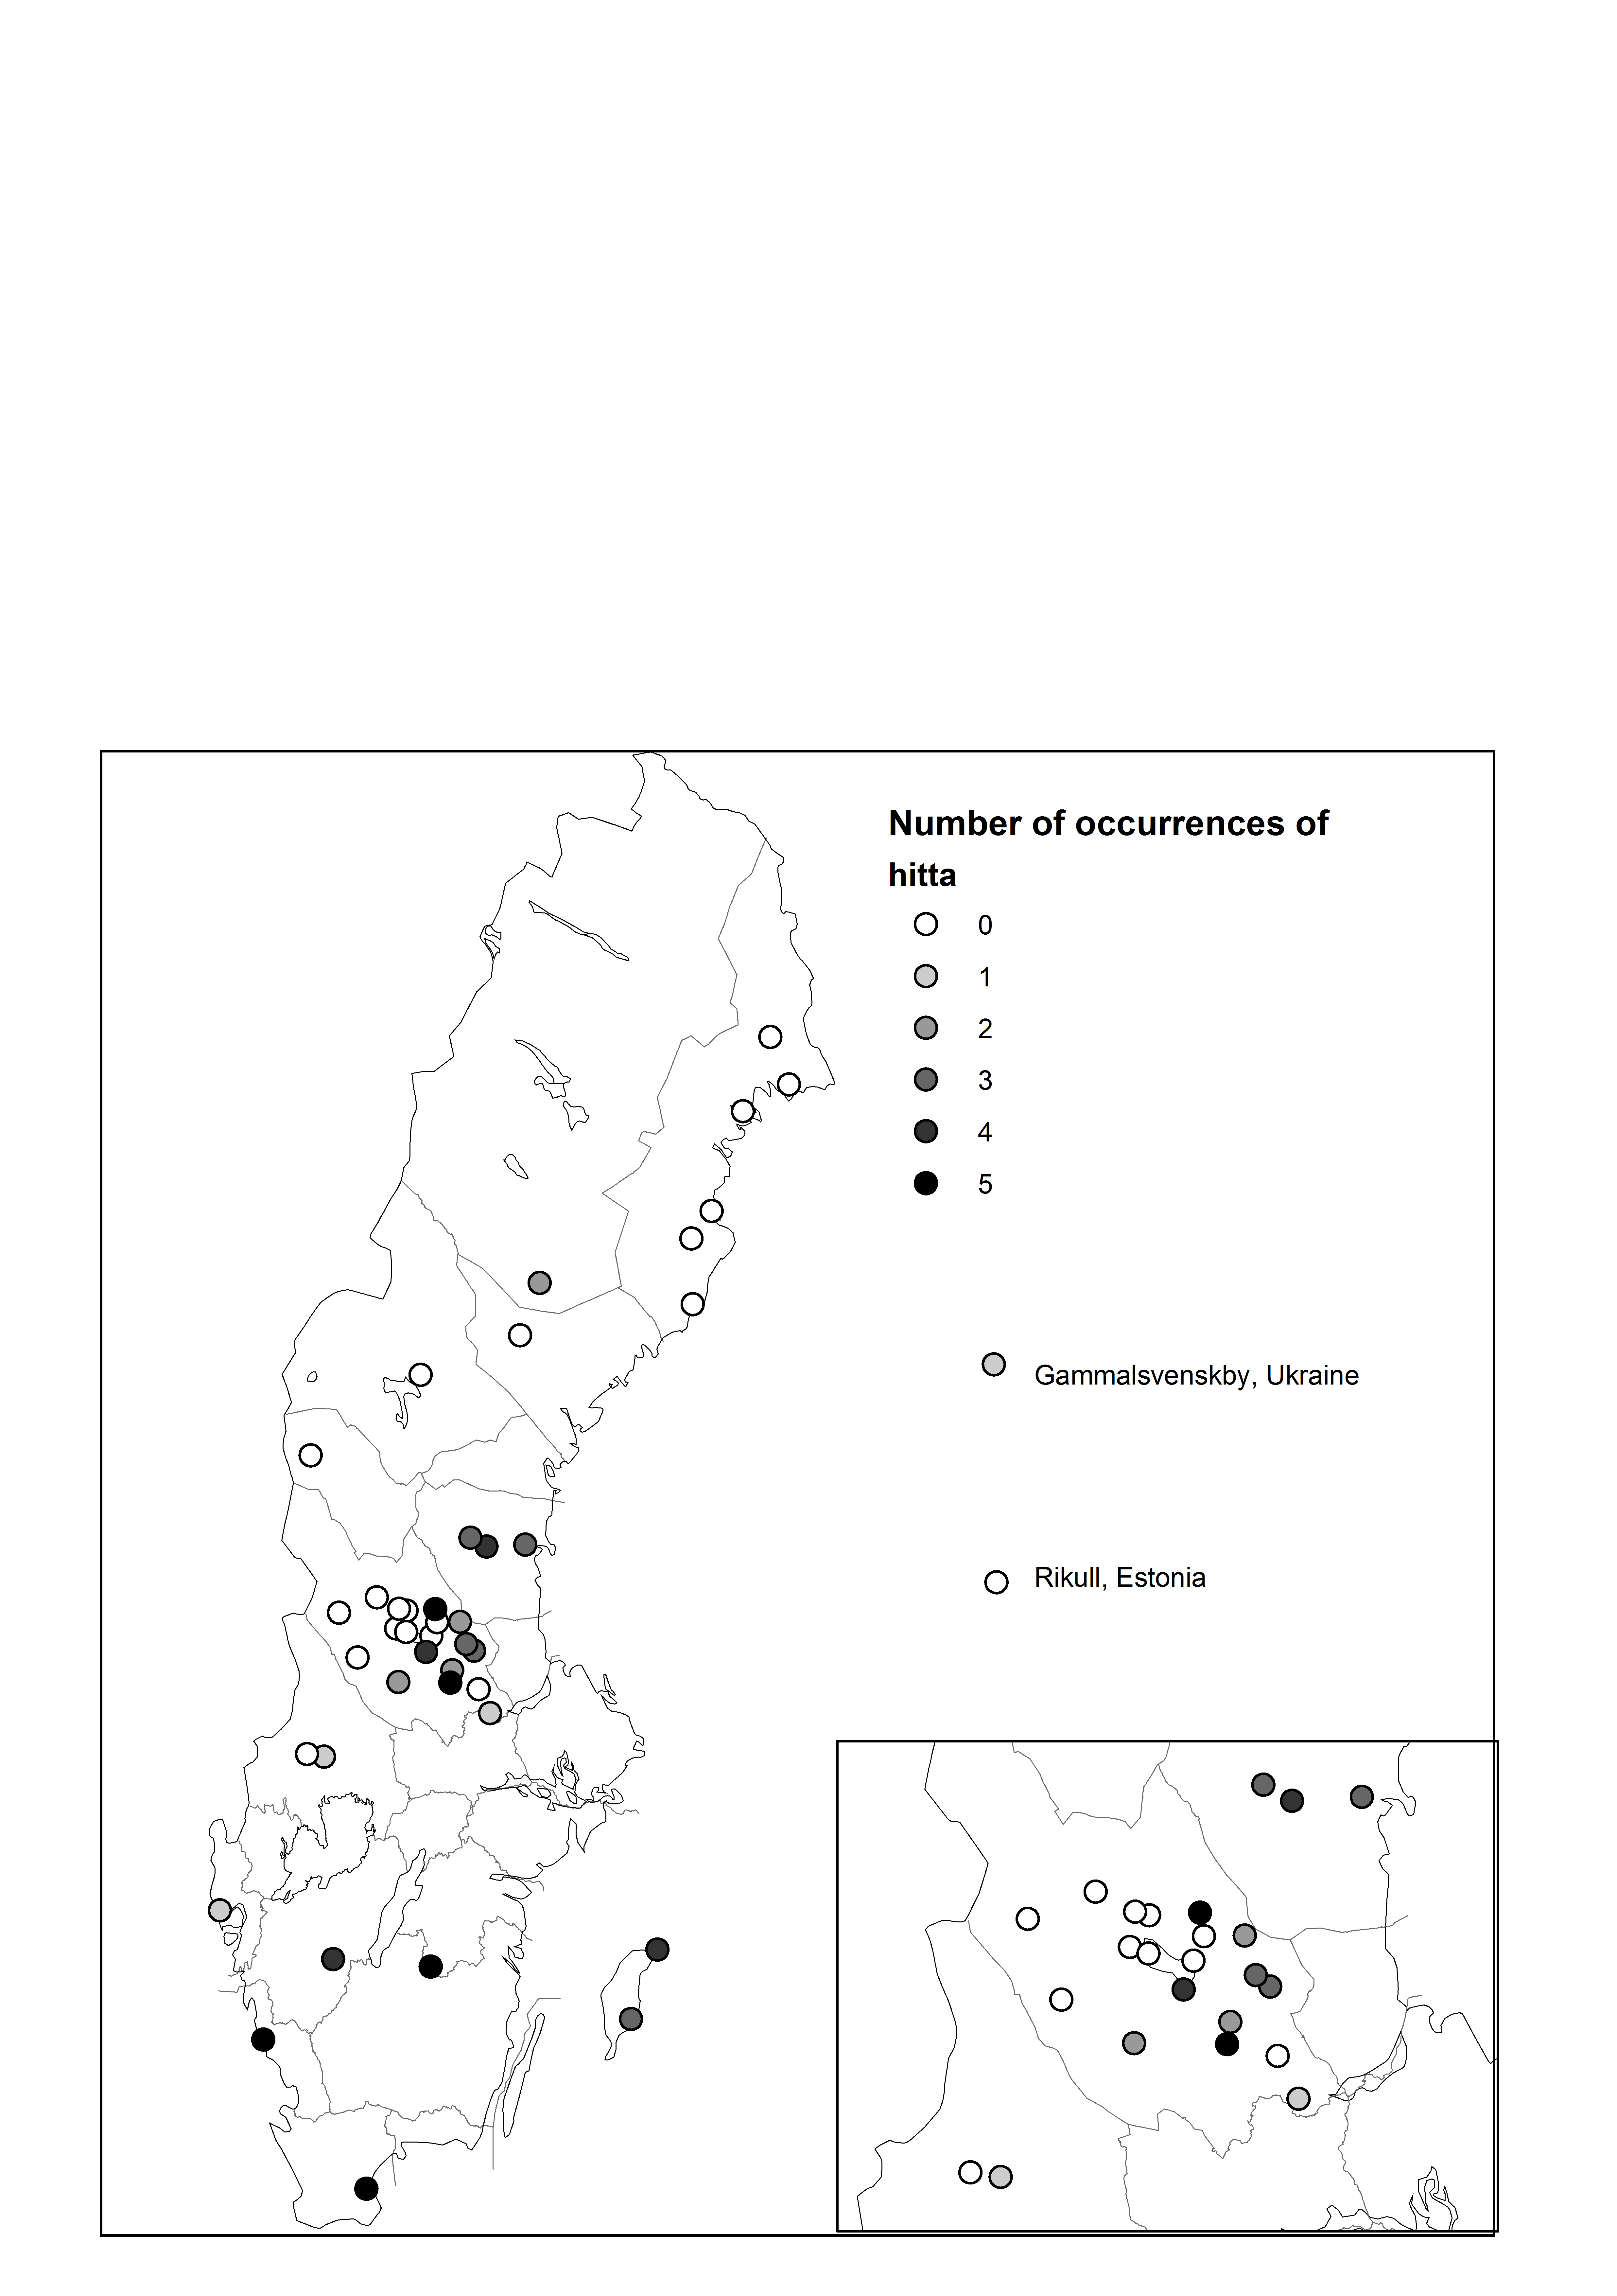
\includegraphics[height=.5\textheight]{figures/37_DistributionofHitta}
\caption{Distribution of \textstyleLinguisticExample{hitta} in Cat Corpus.}
\label{map:33}
\end{figure}
   
\section{The conservativity and innovativity indices}

We have looked at a number of “archaisms” and a number of innovations in the Peripheral Swedish area. Their distributions are not identical, but certain tendencies are visible and can be made even clearer by assigning two indices to each parish: one index of “conservativity” and one of “innovativity”, depending on how well the two types of features are represented in the vernacular in question. The definition of a conservative trait is one that is shared by the vernacular and the assumed common ancestor of all varieties in the Swedish dialect area, but which is not found in modern Standard Swedish. The definition of an innovative trait is one that is found neither in the assumed proto-language nor in modern Standard Swedish – and therefore must be assumed to have arisen through an innovation. 

The following features enter into the conservativity index:

\begin{itemize}
\item 

Preservation of original \textit{a} in positions where it has become \textit{å} in Swedish

\item 

Preservation of dative and/or accusative case in nouns

\item 

Preservation of original diphthongs

\item 

Preserved long stem vowels in cognates of Swedish \textit{natt} ‘night’ and \textit{döma} ‘judge’

\item 

Absence of temporal subjunction \textit{när}

\item 

No palatalization of \textit{k} and \textit{g} before front vowels in initial position

\item 

Absence of preposed definite article

\item 

Retainment of \textit{varda} paradigm

\item 

Preservation of \textit{w}
\end{itemize}
 

The following features go into the innovativity index:

\begin{itemize}
\item 

Presence of demonstratives of the type\textit{ han där} and \textit{he där}

\item 

Absence of neutral pronouns \textit{(h)ä(d)}

\item 

Presence of diphthongs \textit{ie} and \textit{yö}

\item 

Apocope

\item 

\textit{Pp} instead of \textit{mp }in words such as \textit{sopp} ‘mushroom’

\item 

Generic use of pronoun \textit{han}

\item 

Adjectival incorporation

\item 

Deletion of \textit{h}

\item 

\textit{(H)jär} ‘here’

\end{itemize}

The result is shown in Maps 34-35. 

\begin{figure}[h]
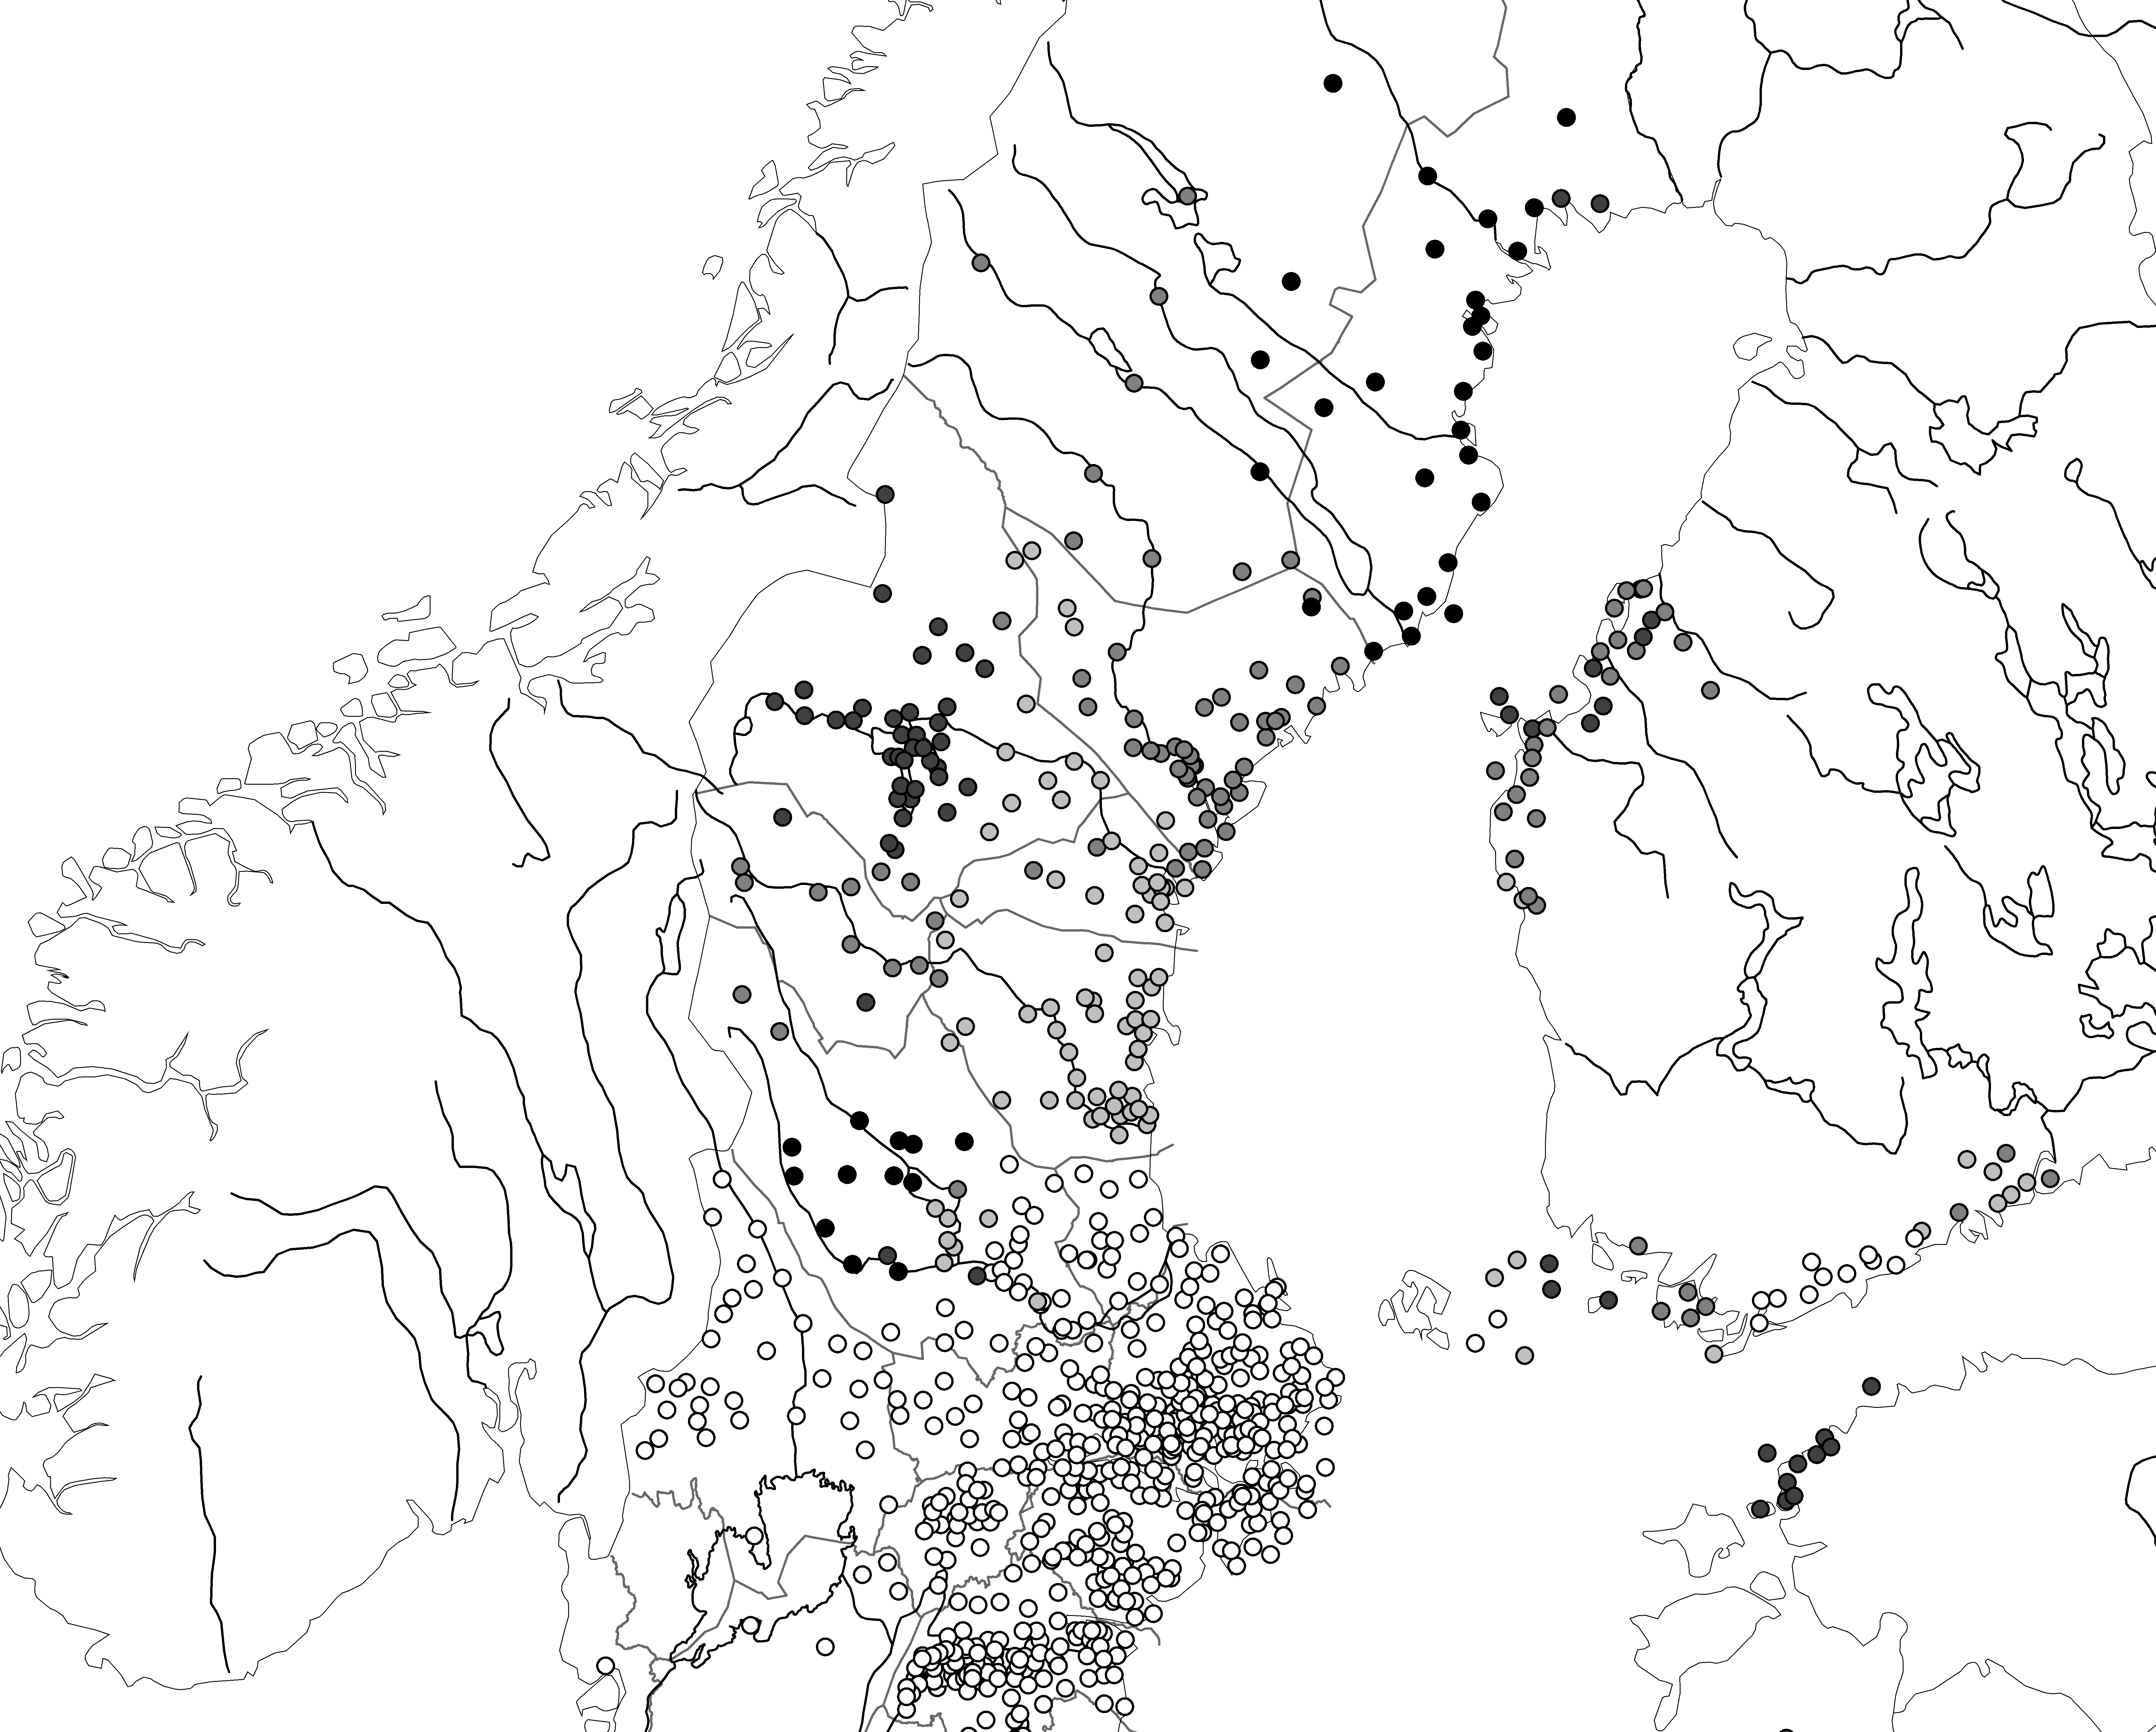
\includegraphics[height=.5\textheight]{figures/38_DistributionConservativeFeatures}
\caption{Distribution of conservative features in central and northern parts of the Swedish dialect area (darker circles -{}-higher conservativity index). }
\label{map:34}
\end{figure}

\begin{figure}[h]
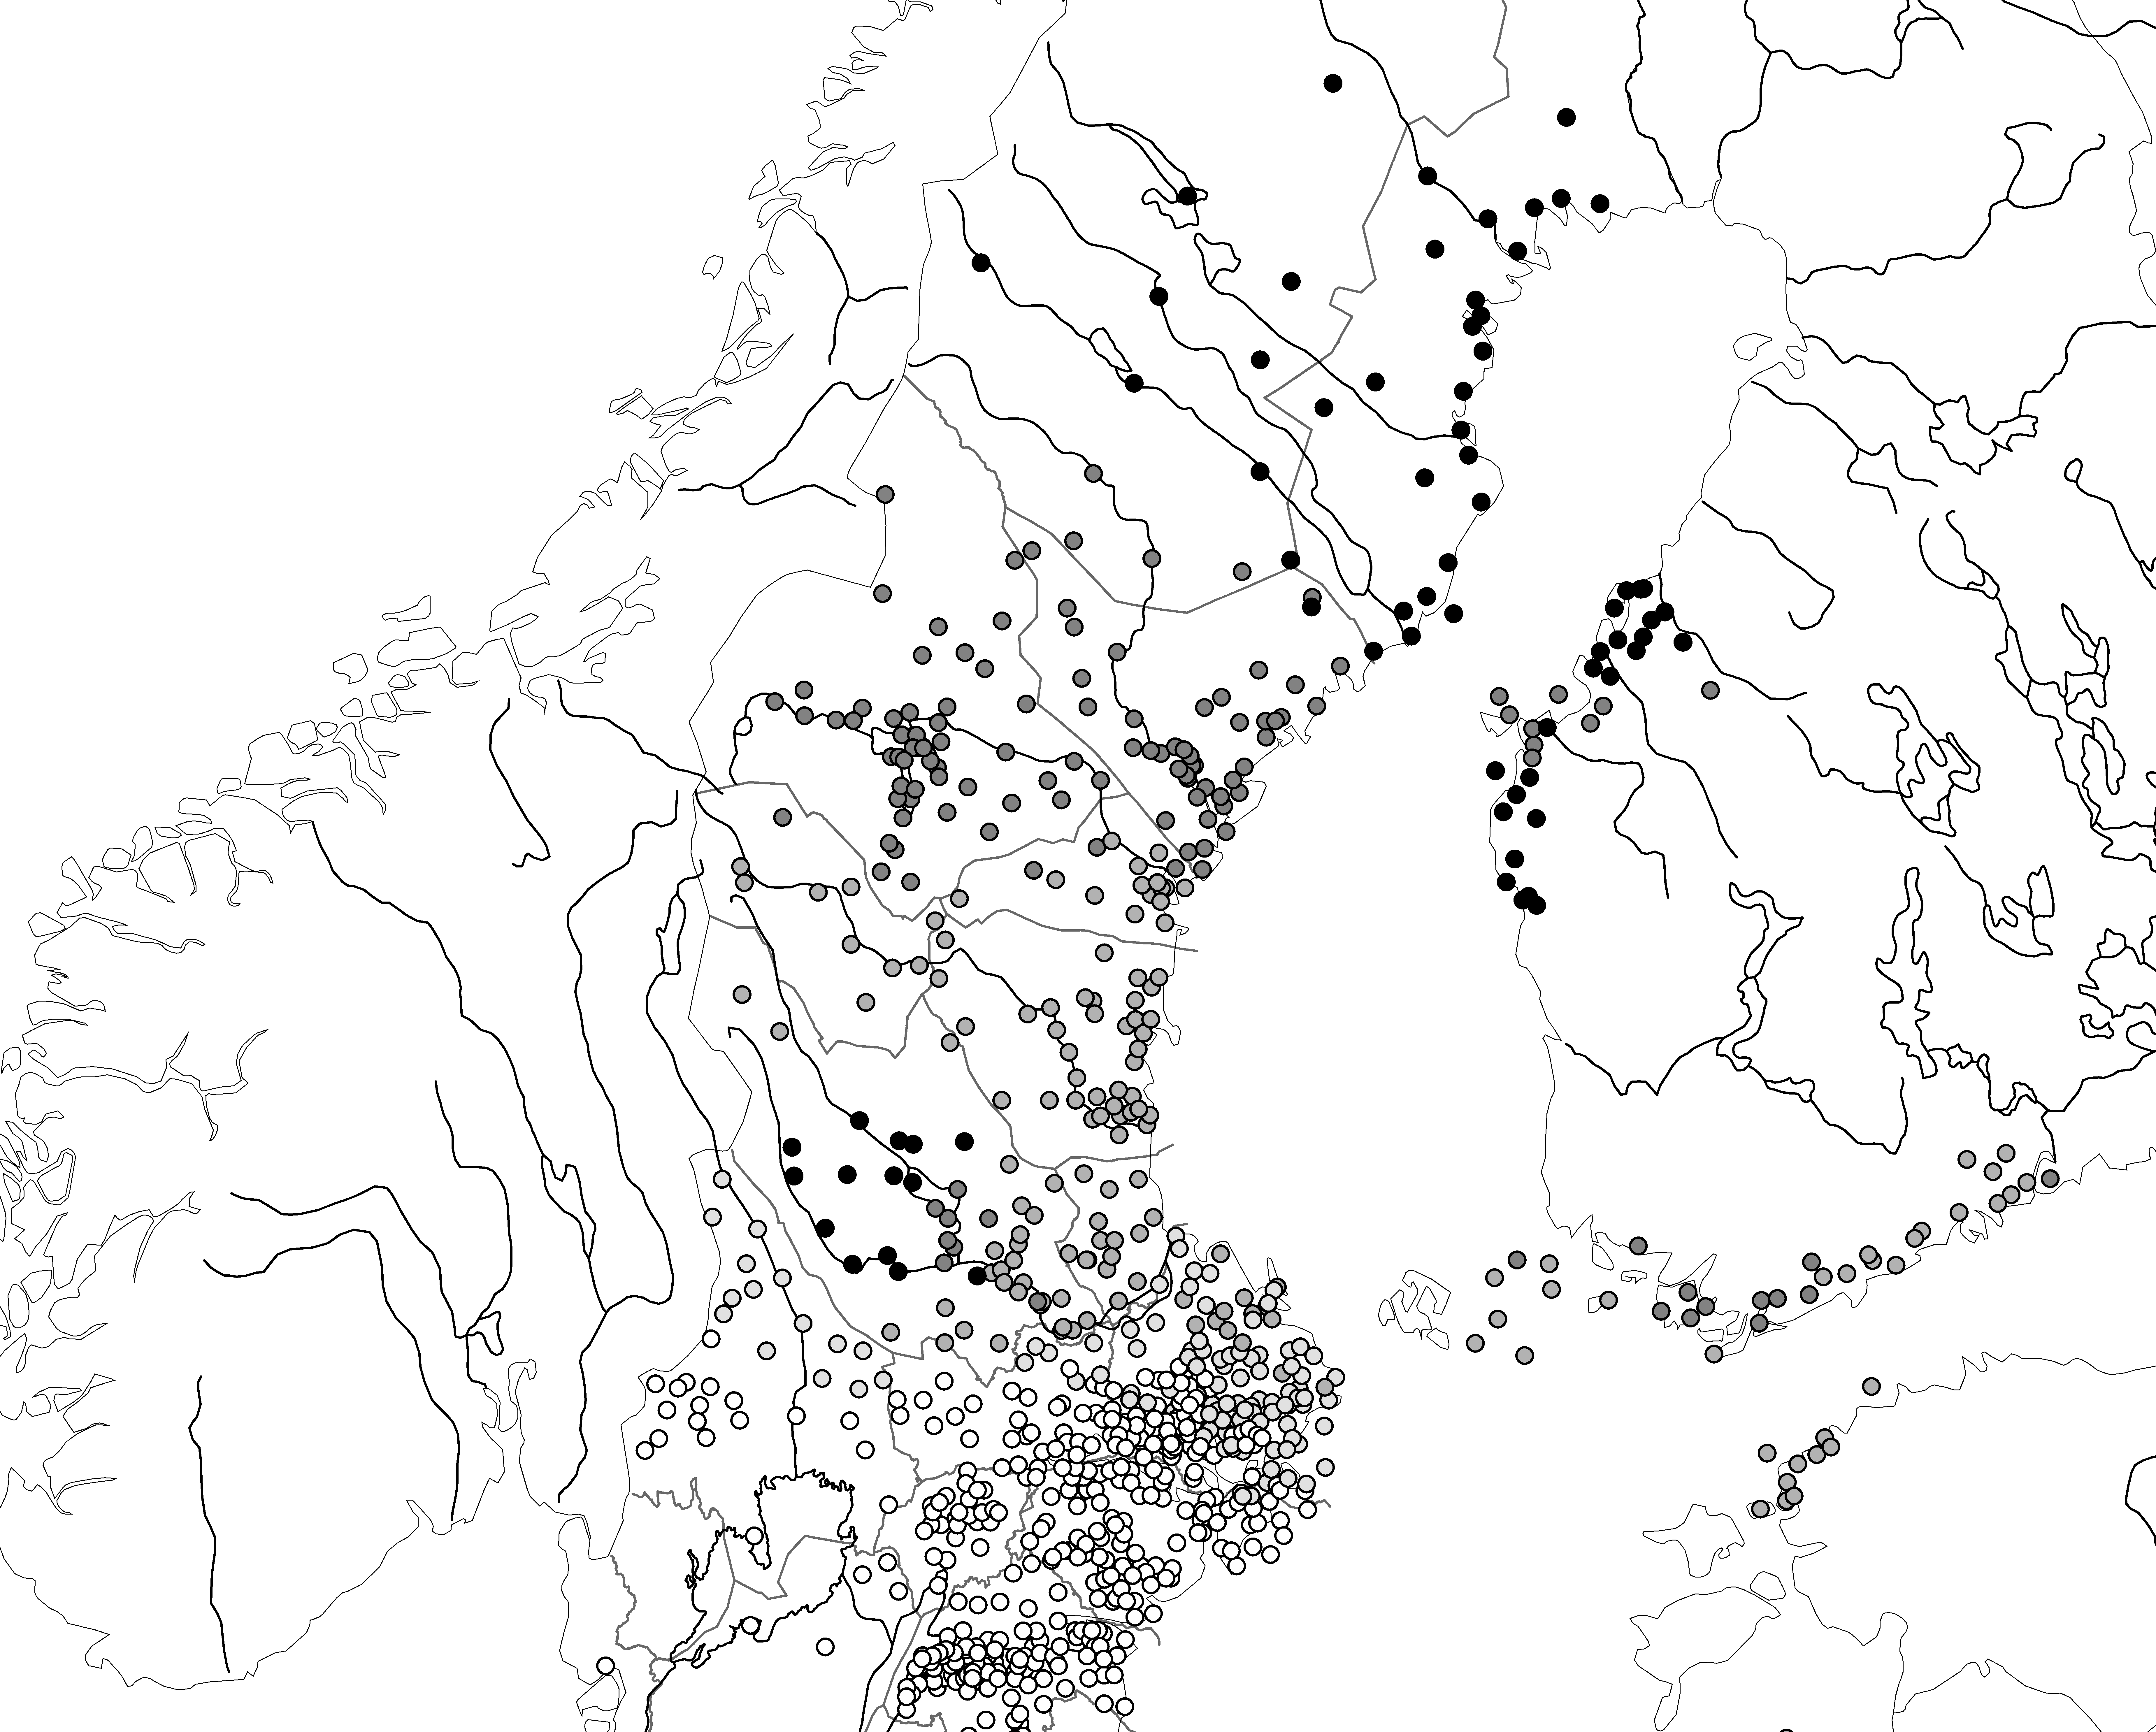
\includegraphics[height=.5\textheight]{figures/39_DistributionInnovativeFeatures}
\caption{Distribution of innovative features in central and northern parts of the Swedish dialect area (darker circles -{}-higher innovativity index). }
\label{map:35}
\end{figure}
 
 
As can be seen, the maps are similar enough for it not to be immediately obvious which map corresponds with the distribution of conservative vs. innovative features. From a visual inspection, conservativity and innovativity seem to be highly correlated. The correlation index turns out to be 0.62, which is perhaps not so impressive, but rises to 0.86 if we compare averages in dialect areas rather than values for individual parishes. The darkest areas of the maps are in Ovansiljan, northern Västerbotten and, to a lesser extent, Norrbotten. The most pronounced differences between the maps are found in Jämtland, which is more conservative than innovative, and Ostrobothnia, which is the other way around. 

What conclusion should be drawn from the similarity between the maps? In my opinion, the most parsimonious way of explaining the parallels between the conservative and the innovative features is that they originally had a shared larger distribution but were later pushed back by essentially the same kinds of processes. This means that the innovations must be old enough to have already been in place when these processes occurred. Given the general geographical picture, it appears that both the original spread of the innovative features and the later processes that obliterated them started in the same region, viz. in the Mälar provinces. 

Now, an objection may be raised that the choice of features is somewhat arbitrary. As for the conservative traits, I have mainly tried to choose ones where there is enough reliable information to make mapping possible, but I do not think it is possible to choose a set of features that would give a radically different picture. For the innovative features, the situation is a bit different. Here, I have to a certain degree deliberately chosen ones that fit the point of view I am arguing for. This is, I think, in fact legitimate insofar as I want to show that there is a coherent set of phenomena that show a definite pattern, suggesting a common history. Other innovations may not fit into that pattern, which can be seen as an indication of a different scenario. In particular, it does seem that certain phenomena spread, not from central Sweden, but rather from Norway. These include the use of preproprial articles and of \textstyleLinguisticExample{h}{}-genitives, two phenomena that most likely are connected with each other. 

\section{Notes on the historical background}
\subsection{Medieval Sweden}

According to the traditional view of Swedish history, during the Viking Age, if not earlier, the Svea ethnic group formed a kingdom with its centre in Uppland; this kingdom was fairly soon extended to also include the Göta ethnic group in central Götaland. developments in archaeology and history have modified this picture considerably. It is now thought that a stable central power was established in Sweden very gradually and probably not until the 13\textsuperscript{th} century. The existence of “kings” in Uppland from relatively early times seems well documented, but it is unclear how far their sphere of influence extended. During the 9\textsuperscript{th} and 10\textsuperscript{th} centuries, the town of Birka in Lake Mälaren (which was at this time part of the Baltic Sea) was the commercial centre of the Mälar region and was apparently part of a larger network including Hedeby in southern Denmark (present-day Schleswig-Holstein) and Kaupang in Norway. Around the turn of the millennium, Birka was replaced by Sigtuna farther to the east. The 11\textsuperscript{th} century is the time when most of the runic stones in Uppland were created. It appears that this was largely due to a “fashion” connected with the introduction of Christianity. There is evidence of Danish influence in Sigtuna during this period. According to the traditional account of the history of the Scandinavian languages, this was the time-point of the split between “East Nordic”, comprised of Danish and Swedish, and “West Nordic”, comprised of Norwegian and Icelandic. As I noted in \citet{Dahl2001}, the fact that Swedish and Danish seemed to go the same way – that is, that the same innovations were introduced in both Denmark and Sweden at the same time – is difficult to explain without assuming very intensive contact between the countries. It may be speculated that, in the Mälar provinces with Sigtuna as the centre, the introduction of Christianity was accompanied by the spread of a prestige dialect heavily influenced by Danish. 

The 12\textsuperscript{th} and 13\textsuperscript{th} centuries are somewhat paradoxical in the sense that the “Svea” kings were mainly based in Götaland, with power alternating between the leading families of Västergötland and Östergötland. It appears that since the royal title carried considerable prestige, it was a useful resource when consolidating the developing central power in Götaland even if it was associated historically with the Mälar provinces. At the same time, these provinces were less centralized, and the ruling group of magnates (\textstyleLinguisticExample{stormän}) there was apparently quite happy as long as the person who was nominally their King stayed in Götaland and did not interfere in their affairs. The process of Christianization went considerably faster and apparently more smoothly in Götaland than in Svealand. The fact that Svealand and Götaland had different monetary systems until the end of the 13\textsuperscript{th} century is another sign of the incomplete integration of the two regions. In fact, most of the visible events in Swedish history during this period took place in Götaland – one gets the impression that the Mälar provinces were some kind of backwater. At any rate, there is very little written documentation from this period. 

On the other hand, it does seem fairly clear that the Mälar provinces had a central part in one major economic and demographic development during this period, viz. the expansion of agriculture. \figref{map:36} shows the growth of permanently settled areas in Sweden from the Late Iron Age to the Late Middle Ages. As can be seen, it was during this period that large parts of the Peripheral Swedish area were settled. The same goes for the Swedish-speaking areas on the other side of the Baltic, which are not shown on the map. At least for the newly settled areas in Northern Sweden, it is probable that they received most of their new population from the Mälar provinces. Even areas that were already settled in the Iron Age, such as the peripheral parts of Uppland and the Middle Norrlandic provinces, greatly increased their population during this time (\citet{Broberg1990}), and it is reasonable to assume that there was considerable immigration from the central provinces. 

At least for the northernmost parts, the expansion seems to have continued during the first half of the 14\textsuperscript{th} century, when officially sanctioned colonization of the Lule and Pite river valleys took place, maybe in order to prevent Russian expansion plans in the area, and partly pushing back earlier Finnish settlements. In general, the expansion can be assumed to have been halted by the general agricultural crisis at the end of the Middle Ages, traditionally connected with the Black Death and a deterioration of the climate, and was not resumed until the 16\textsuperscript{th} century (\citet[248]{Myrdal2003}). Before this, however, other important things had happened.

Whereas the political leaders of Götaland had shown a certain lack of interest in Svealand in the 12\textsuperscript{th} and the beginning of the 13\textsuperscript{th} century, this changed under Birger Jarl, who was never King but effectively ruled Sweden as “jarl” during the years 1248-1266. He belonged to a leading family of Östergötland but is probably most well-known as the alleged founder of Stockholm, although his role in this may have been slightly exaggerated. (The continuous rise of the land had given Stockholm a very strategic position, since this was now the only entrance to Mälaren from the Baltic.)

What is clear is that Birger Jarl used quite brutal means to take control over the Mälar provinces, and that he realized the economic potential of this region, concluding among other things a treaty with the Hansa city Lübeck in order to promote the development of trade relations. The Mälar region was rapidly urbanized (see Map ). There were also considerable numbers of German merchants in the towns, and Low German was extensively used. German immigrants were also attracted to the Central Swedish mining district (“Bergslagen”), which was gradually growing in importance. A major factor in this development was the copper mine in Falun in southern Dalarna. At the same time, the previously quite important production of iron from bog and lake ore in northern Dalarna lost its significance. This may have contributed to the isolation of this area which in its turn may have cemented the linguistic differences between the Dalecarlian vernaculars and the rest of the Swedish dialect area. 

In the 14\textsuperscript{th} century, Denmark’s political influence grew, and in 1389, Denmark, Norway and Sweden were united in the Kalmar Union, which officially lasted until 1521, although in practice, Sweden was out of control for long periods. 

Turning now to linguistic developments during the Middle Ages, there is a virtual break in the record between the runic stones of the 11\textsuperscript{th} century and the first longer texts in Latin script in the 13\textsuperscript{th} century, although there is evidence for a continuous tradition of writing with runes (mainly on wood). From the 13\textsuperscript{th} century there are mainly provincial laws, the first longer text in Latin script emanating from the Mälar provinces is the Upplandic Law, which was promulgated by the King in 1296. (“Dalalagen” may be the oldest text from Svealand but its status is unclear.) 

The centre of the development of Written Medieval Swedish seems to have been Östergötland, more specifically the south-west part around the town of Vadstena, which was also the origin of the ruling families of the province. \citet[53]{Wessén1966} says that the Written Medieval Swedish was coloured by the Östergötland dialect\footnote{ “fornsvenskt skriftspråk är östgötskt färgat; det är väsentligen Vadstenaspråk” }, but one may surmise that it was the language of the élite that played the major role rather than that of the rank-and-file population. There has been little discussion of possible social variation in the language during this period, but given that society was highly stratified and that the ruling groups had intimate connections outside the area, it is to be expected that there were quite significant differences between the social classes. But Written Medieval Swedish, in particular the language of the legal texts, may also reflect older writing traditions.

There is relatively little dialectal variation in the provincial laws. This could be taken as an indication of the absence of such variation also in the spoken language, but in my opinion it rather suggests that there was in fact a relatively standardized way of writing such documents. We should therefore not expect, for example, the Upplandic Law to reflect spoken 13\textsuperscript{th} century Upplandic to any great extent. After all, it was produced by a royal commission (headed by Birger Persson, father of Saint Birgitta, recently appointed the Patron Saint of Europe). 

The strongest factor determining the further development of Swedish was undoubtedly the urbanization process and the development of trade relations. The strong influence of Low German on all the Scandinavian languages during this period, especially the vocabulary, is well known. Undoubtedly, the population of many Swedish towns was ethnically quite mixed, with a large proportion of Germans. It is also often pointed out that at least in Stockholm there was a fairly large number of Finnish speakers. It is highly probable that special urban varieties would have arisen in the Swedish towns and would have differed quite considerably from the ways people spoke in the surrounding countryside. Scholars such as Elias \citet{Wessén1954} have spoken of a “mixed language” as a result of German-Swedish contacts. But it is also likely that there were other non-local influences, since the population of the rapidly growing towns in the 13\textsuperscript{th} and 14\textsuperscript{th} century Mälar provinces would have also been recruited from other parts of Sweden. Birger Jarl’s taking control of the Mälar provinces must also have meant a movement of people from Östergötland to Stockholm and other towns in the area, and this may have especially had consequences for the prestige variety.

In addition, the role of Danish has probably been underestimated. The 19\textsuperscript{th} century scholar Esaias Tegnér, Jr. voiced the opinion that “even if, as is natural, Swedish received many loans directly from German during the Low German period…, it is the Danish influence during the period of the Kalmar union which to a quite essential extent has contributed to the establishment of such Low German words and to the form in which they appear”.\footnote{ “En granskning af de tyska lånorden i vårt språk har bibragt mig det intrycket, att om ock svenskan naturligtvis under den lågtyska perioden (intill reformationstiden) mottagit många lån omedelbart från tyskan, så är det likväl i ganska väsentlig grad danskarnas inflytande i Sverige under Kalmarunionens tid, som bidragit därtill att dylika lågtyska ord blivit bofasta hos oss och att de uppträda i den form, som vi finna dem hava.” (\citet[159]{Tegnér1889})} Tegnér points to the high degree of correspondence between the Low German grammatical and lexical elements in Danish and Swedish and to the fact that the same deviations from the original Low German forms tend to show up in both languages. Such differences that are found, he says, are usually attributable to later High German influences. I checked Tegnér’s claims by looking at the words listed as Low German loans in \citet{Hellquist1922}; as it turns out, a very high proportion (perhaps something like 90 per cent) do exist or have existed also in Danish. Scholars after Tegnér, however, have not paid too much attention to his hypothesis. \citet{Wessén1954} is sceptical: according to him, the high degree of correspondence, which he does not deny, can be explained by the common “cultural and linguistic preconditions” for borrowings in Danish and Swedish. I would personally tend to side with Tegnér on this issue. It is, furthermore, possible to establish quite a long list of points where Standard Swedish and urban Central Swedish join Standard Danish against most of the vernaculars in Peninsular Scandinavia, at least those north of the Southern Swedish/East Danish dialect area, such as the restructured gender system, the feminine definite suffix\textit{ {}-}\textstyleLinguisticExample{en}, the use of \textstyleLinguisticExample{att} (rather than \textstyleLinguisticExample{till}) as an infinitive marker and \textstyleLinguisticExample{man} as a generic pronoun, consistent preposed placement of possessive pronouns etc. 

It is commonly said that Standard Swedish arose from the dialects of the Mälar region, but it is often not made clear exactly which these dialects were. \citet[67]{KällskogEtAl1993}, in their discussion of the similarity between Standard Swedish and Upplandic, claim that the base for the former is to be found in medieval “high-status dialects, primarily Upplandic and \textit{östgötska} [the speech of Östergötland]”.\footnote{ “Stommen i detta språk utgjordes av folkmål med hög status, främst uppländska och östgötska…”} Thus, they say, it is not the case that Upplandic has been influenced by the standard language in Stockholm and Uppsala, it is rather the other way around. The Swedish expression they use for ‘high-status dialects’, “folkmål med hög status”, sounds almost like an oxymoron, given that “folkmål” is usually understood as denoting rural, non-standard varieties. In fact, their claim does not make a lot of sense if the flow of influence is not supposed to go from rural to urban varieties. In the next section, we shall look more closely at the dialect situation in Uppland.

\begin{figure}[h]

\begin{overpic}[scale=.5,unit=1mm]%
{figures/40_GrowthofPermSettled_small.png}
\setlength{\fboxsep}{0pt}
\put(66,20){
  \framebox[3cm]{
    \parbox{2.8cm}{
      \smallskip
      
      Late Iron Age \mbox{settlements}   \fbox{\color{black!80!white}\rule{1em}{1em}}
      \bigskip

      Late Middle Age settlements \fbox{\color{black!40!white}\rule{1em}{1em}}
      \bigskip

      Adapted from the Swedish National Atlas
      \smallskip
      
    }
  }
}
\end{overpic}

% \includegraphics[height=.5\textheight]{figures/40_GrowthofPermSettled}
\caption{Growth of permanently settled areas between approx. 800CE and 1350CE. }
\label{map:36}
\end{figure}

\begin{figure}[h]
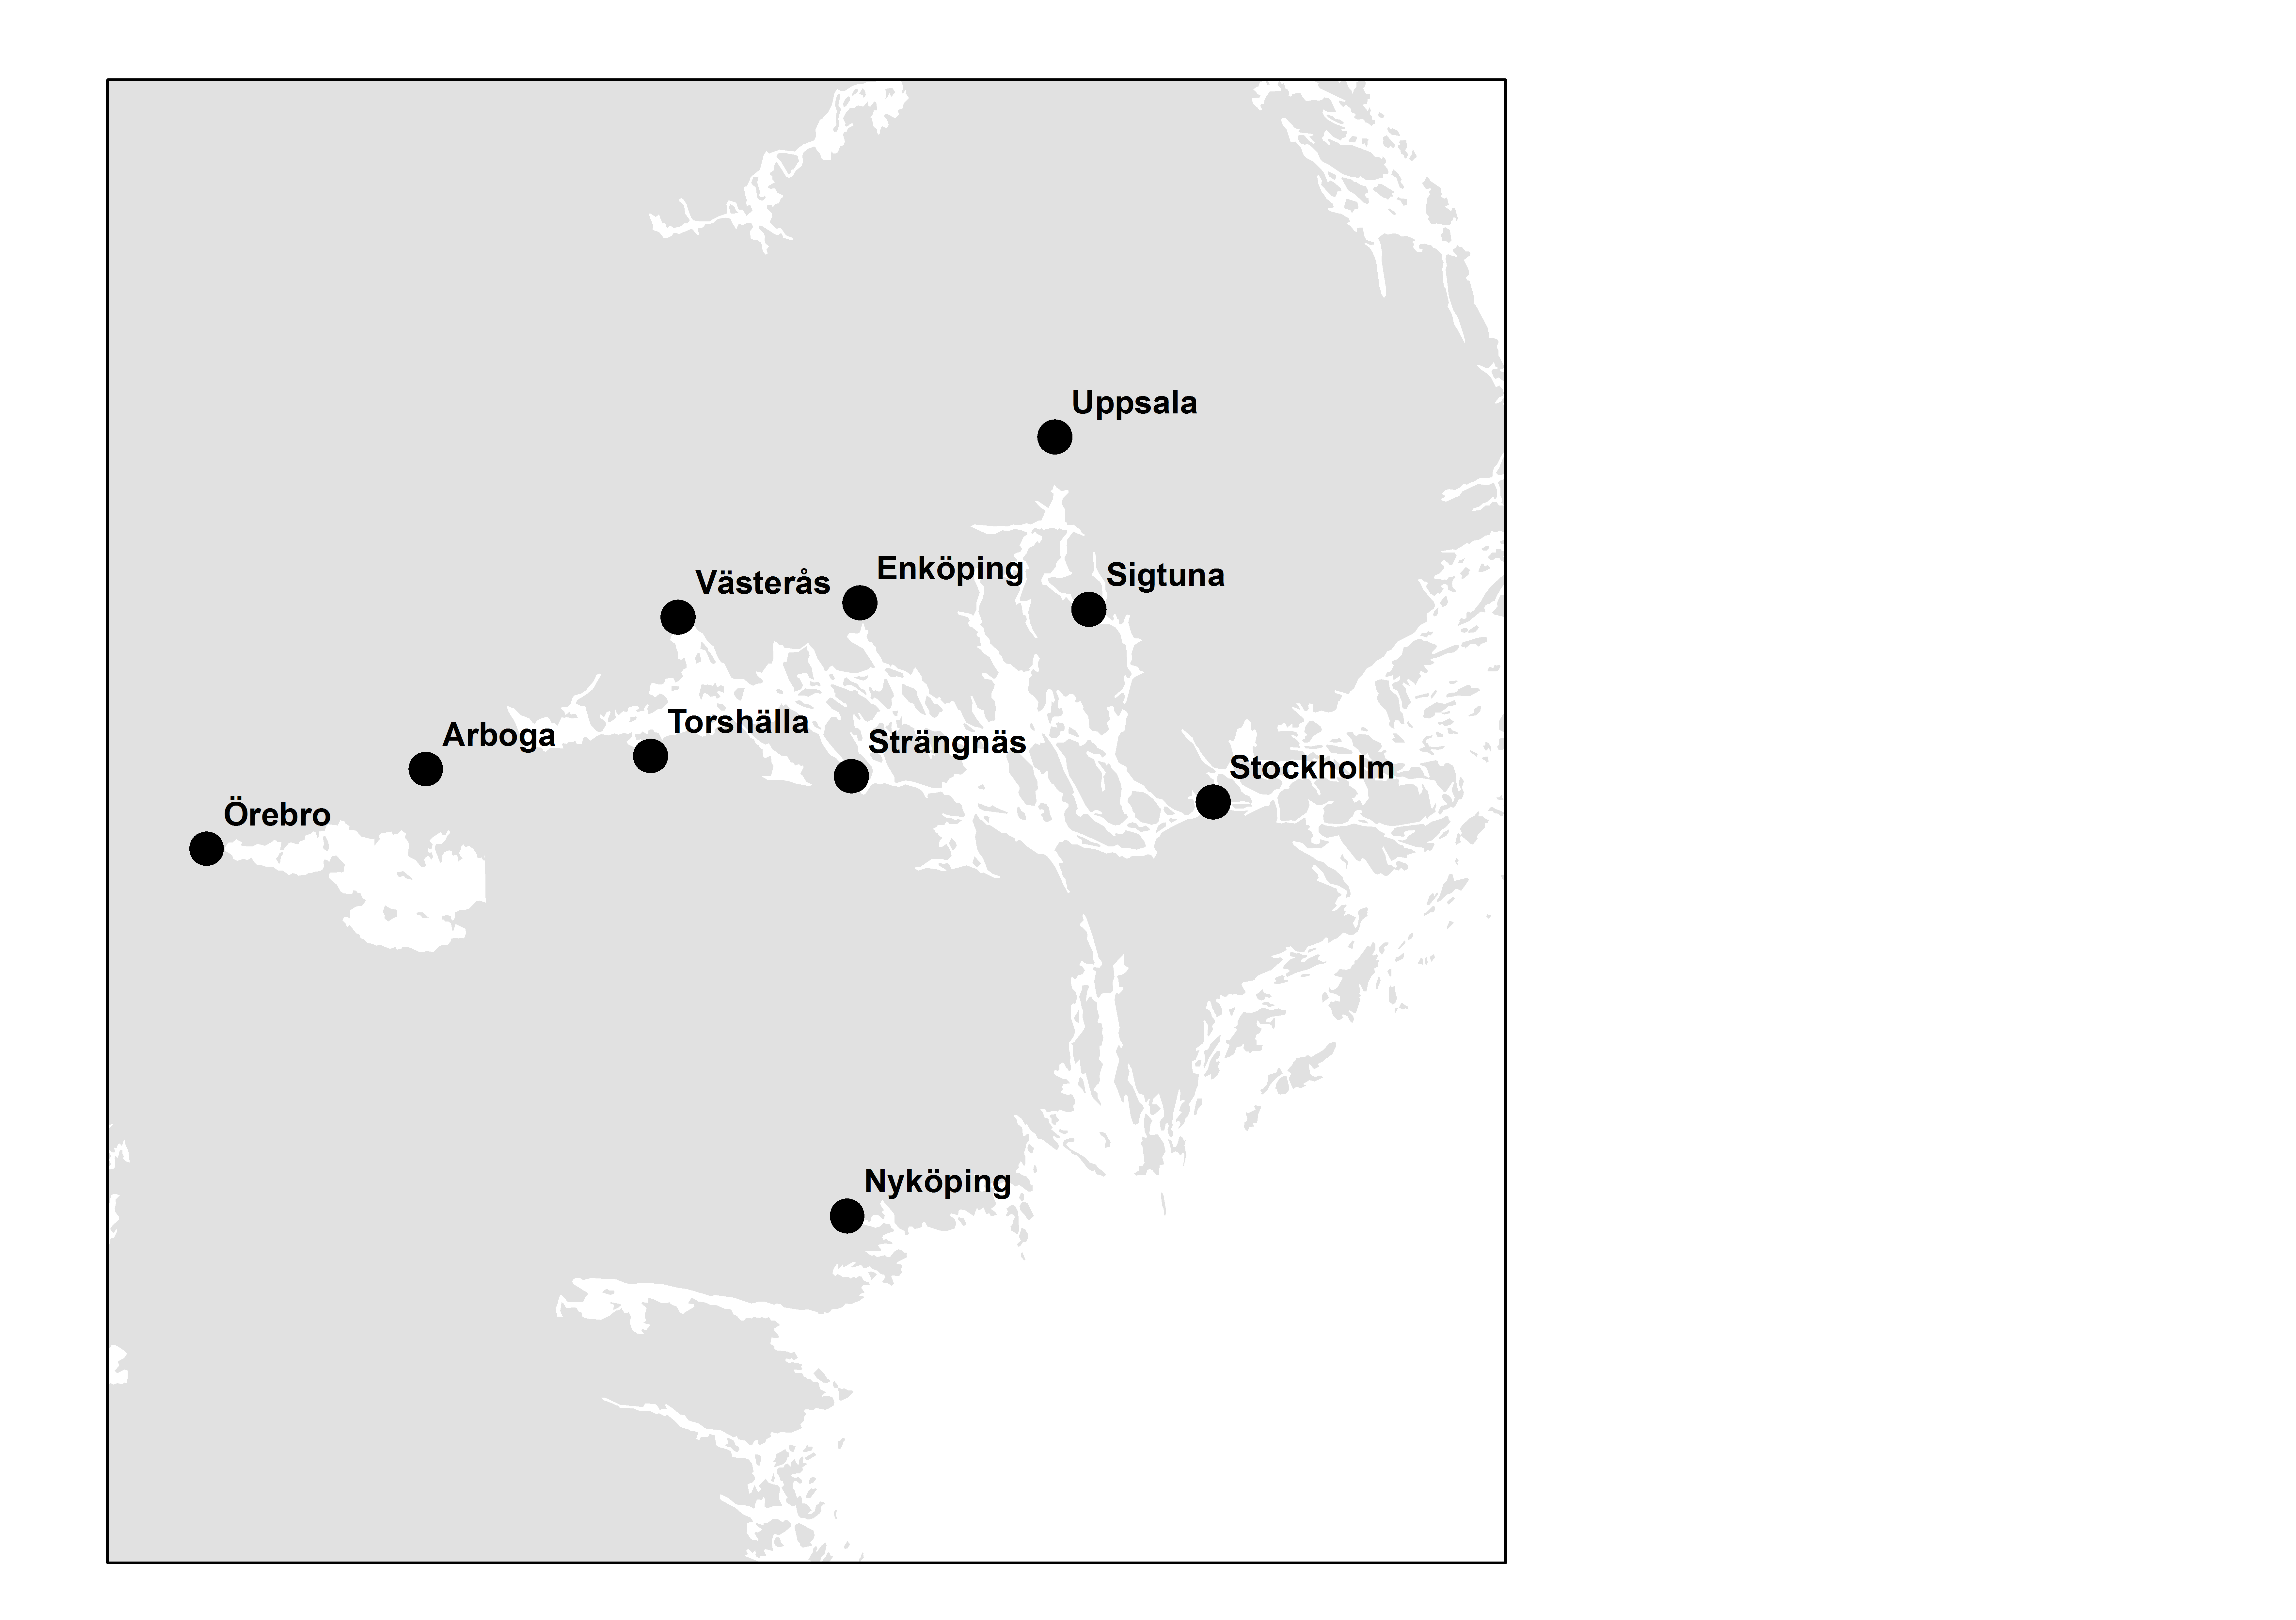
\includegraphics[height=.5\textheight]{figures/42_CitiesandTowns}
\caption{Cities and towns in the Mälar region  in the late 13th century. }
\label{map:37}
\end{figure}

\begin{figure}[h]
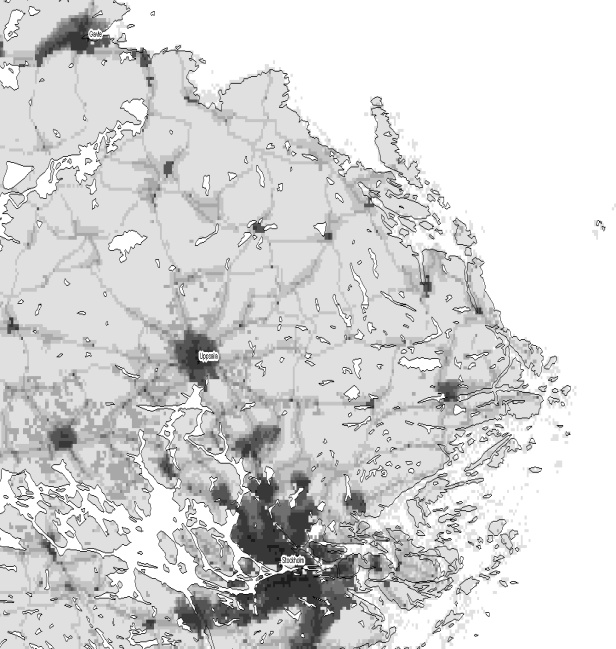
\includegraphics[height=.5\textheight]{figures/43_PopulationUppland}
\caption{Distribution of population in present-day Uppland.}
\label{map:39}
\end{figure}

 
\begin{figure}[h]
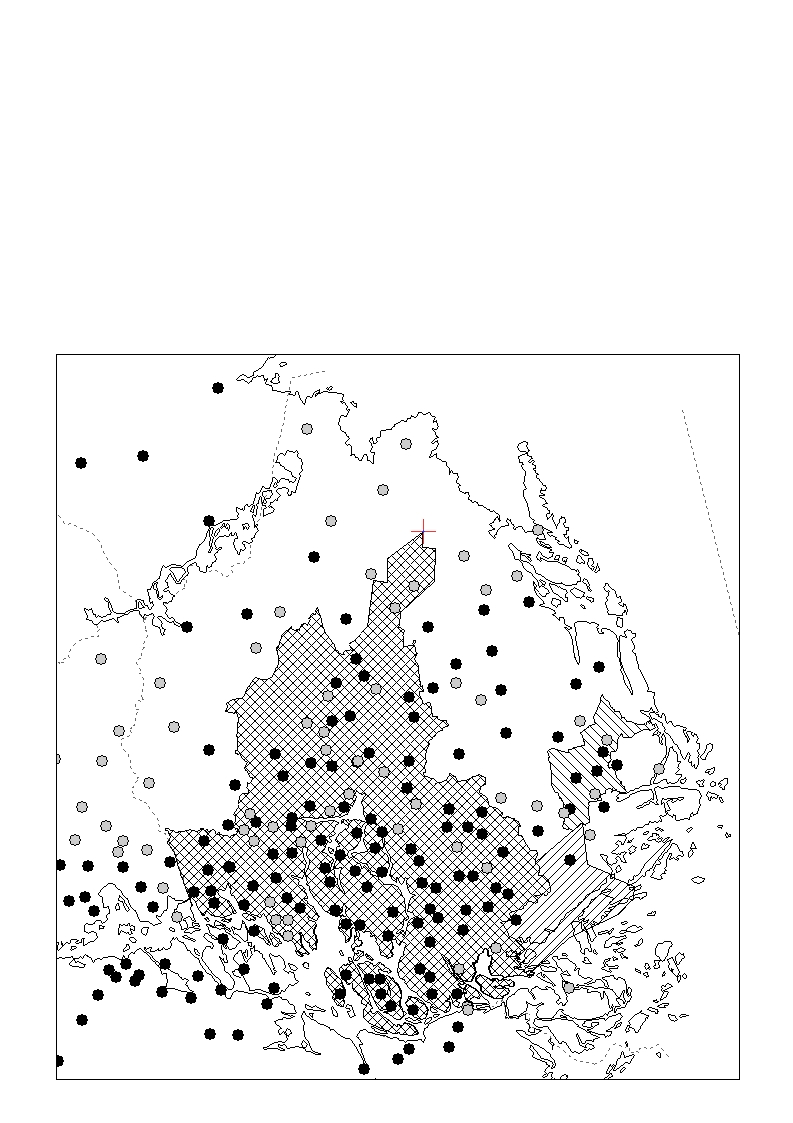
\includegraphics[height=.5\textheight]{figures/44_UpplandHighActivity}
\caption{Uppland with “high-activity” areas  and medieval churches (black circles represent churches built 1000-{}-1250, grey circles churches built 1250-1500; left hatching  {}-{}- hundreds with {\textgreater}20 runic stones, right hatching  {}-{}- {\textgreater}50 per cent land with tax-relief in the mid 16\textsuperscript{th} century).}
\label{map:38}
\end{figure}

  

\subsection{Uppland}

To understand the dialectological situation in Uppland, it is of some importance to relate it to the administrative and demographic structure of the province.

The present-day province of Uppland has, strictly speaking, never functioned as an administrative unit. The judicial province (\textstyleLinguisticExample{lagsaga}) of Uppland that was created in 1296 also included the province of Gästrikland, and was formed by merging three so-called “folklands”, Fjädrundaland (Fjärdhundraland), Tiundaland, and Attundaland. These names mean “the land of four (ten, eight) hundreds” and refer to the number of \textstyleLinguisticExample{hundare}\textstyleLinguisticExample{,}\footnote{ The word \textit{hundare} corresponds etymologically to English \textit{hundred}\textit{,} used in medieval England as a term for a division of a shire The \textit{hundare} were later on identified with the judicial districts called \textit{härad}.} smaller administrative units, suggesting that the names were created as a bureaucratic measure from above rather than developing naturally. The coastal region nowadays called Roslagen had a somewhat uncertain status: it was divided into two halves, referred to as “Norra Roden” and “Södra Roden”, and loosely attached to Tiundaland and Attundaland, respectively. 

The population of Uppland has always been unevenly distributed. \figref{map:39} shows the present-day situation, with a heavy concentration in the urban areas around Stockholm and Uppsala. The medieval distribution was not that different, in fact. The hatched areas in \figref{map:38} (after \citet{Broberg1990}) show the following indicators of social stratification (and thus, presumably the areas with the greatest economic activity and densest population) in earlier times: (i) the hundreds with more than 20 runic stones, (ii) the hundreds which had more than 50 per cent land with tax-relief (that is, land owned by the state, the church or the nobility) in the mid 16\textsuperscript{th} century. It is somewhat remarkable that these two indicators coincide almost completely, and are not too different from what we find today. 

\figref{map:38} also shows the medieval churches in the area, according to the database of the Swedish National Heritage Board (\href{http://www.raa.se}{{www.raa.se}}). These data are of some interest because they show a possible model for the way linguistic innovations may have spread in this period. We can see that there is a concentration of early churches in the southern part of the hatched area, whereas church construction in the Late Middle Ages took place to a much larger extent in the peripheral areas.

The conclusion that can be drawn is that medieval Uppland, like Uppland of today, can be understood as having consisted of a centre in the middle south, in the areas adjacent to Lake Mälaren, and a periphery around it. Crucially, this persistent division cross-cuts the old administrative division into folklands, as can be seen when comparing \figref{map:38}-\figref{map:39} with \figref{map:40}. The structure of Uppland is somewhat like (half) a pizza, with each folkland representing one slice, all of which meet in the most densely populated area in the south in the immediate vicinity of the medieval towns Uppsala and Sigtuna. Each folkland itself thus consists of a central and a peripheral part. 

 The first and in some ways still most complete account of the Upplandic dialects is that of \citet{Kruuse1908}.\footnote{ Kruuse says that he bases his account on word lists collected in a survey led by A. Erdmann, in addition to various written works. (The later fate of these word lists is unclear.) } Kruuse is somewhat hesitant to divide Uppland into dialect areas, being well aware that “the area of one linguistic feature very seldom coincides with the area of another, and strictly speaking we cannot speak of a certain number of dialects with definite borders”. After having stated this reservation, he presents a division of the province into four areas, based on a number of important isoglosses. There is a map provided with Kruuse’s article, but it shows the isoglosses rather than the areas – neither Kruuse nor anybody else seems to have drawn a map of the areas themselves, so \figref{map:40} is my own reconstruction from the description in Kruuse’s text. 

A different division is given by \citet[1194]{Hesselman1920} in his article on Upplandic dialects in the encyclopedia \textstyleLinguisticExample{Nordisk familjebok}. He proposes to divide the Upplandic vernaculars “in three larger groups, whose borders by and large follow those of the ancient folklands”.\footnote{ “En god indelning är den, som sammanför upplandsmålen i tre större grupper, hvilkas gränser i stort sedt följa de gamla uppländska folklandens.” } This statement is echoed in later treatments. Thus, in \citet[75]{KällskogEtAl1993}, it is said that Uppland can be divided “into three dialect areas, which to some extent coincide” with the folklands.\footnote{ “Landskapet Uppland kan grovt delas in i tre dialektområden som i någon mån sammanfaller med de tre s.k. folklanden från vikingatid och medeltid…” } The change from “by and large” to “to some extent” may reflect a certain uneasiness on part of the authors. In their ensuing presentation, however, the names of the folklands are used as labels of the three areas, with which they are in practice identified. In my opinion, such a practice is rather misleading. As can be seen from \figref{map:40}, the placement of the borders of the folklands, does not coincide very well with the areas proposed by Kruuse, and indeed, if one looks at the borders of individual phenomena, they tend not to honour the actual folkland borders. What is particularly important here is that three of Kruuse’s areas that “to some extent” coincide with the folklands (Areas 1-3) are actually mainly located on their periphery, while Kruuse’s Area 4 equals the demographic and economic centre of the province, which as we have seen, also includes the pivot points of all three folklands. Note that Kruuse’s Area 4 is wholly included in the central area indicated in \figref{map:38} and in fact follows its borders relatively closely, except in the east. This does not warrant the conclusion that Kruuse’s areas directly reflect the demographic and economic situation in the Middle Ages. The explanation is rather that the centre-periphery division of Uppland has been relatively constant over the last millennium and that it is this division that underlies the modern dialectological make-up of Uppland, being a result of the expansion of innovations from a centre towards a periphery as much as an ancient division into subprovinces. In particular, some of the borderlines drawn by Kruuse may be snapshots of a moving boundary.

\citet[77]{Wessén1966}, having first pointed to the possibility of an influence of “German sound formation and German linguistic habits” on medieval Stockholm speech, says that medieval documents suggest that the spoken language in Stockholm was “to a striking extent” coloured by Central Swedish and Götamål (see \sectref{sec:2.3.2}). (He explains this by immigration from the “inner Mälar provinces”, but does not say where the Göta influence would come from.)

Among the traits characterizing parts of Uppland, there is a subset which shows some interesting and partly baffling characteristics. To start with, most treatments, beginning with Kruuse (or even earlier, in \citet{Rydqvist1868}), tell us that there have been changes in the pitch accent systems in parts of Uppland: the acute accent has been generalized in the northeast (the eastern part of Kruuse’s Area 2), while the grave accent is generalized in large parts of southern Uppland and also in the eastern part of Södermanland (most of Kruuse’s Area 4 and parts of his Area 1, see \figref{map:41}). The generalized grave accent is discussed in some detail in \citet{Nyström1997}.\footnote{ It is not always clear if the generalization means that all words are pronounced with a grave accent or that just more of them are than in the standard language. Thus, Nyström enumerates some standard minimal pairs such as \textit{ánden} ‘the duck’: \textit{ànden} ‘the spirit’ and says that they are all pronounced with a grave accent, and then adds that “also polysyllabic words such as \textit{betàla} ‘pay’, \textit{indiàner} ‘indians’…” are pronounced “more often” with a grave accent. } (For an account of the present-day situation, see \citet{Ericsson2006}). Nyström mentions two logical possibilities: either the grave accent was productive at the time when the definite article became an affix (see \sectref{sec:3.1.4}) and monosyllabic words became bisyllabic through the insertion of a “svarabhakti” vowel, or the generalization is a later innovation, taking place some time between the changes just mentioned and the mid 19\textsuperscript{th} century, when the phenomenon was first documented. In the latter case, which he seems to lean towards, it is plausible to assume, he says, that the generalized grave accent was also found in the urban varieties spoken in Stockholm (as was also suggested by \citet{Otterbjörk1982}) and that maybe Stockholm was in fact the origin of the development. if the contiguous area shown in \figref{map:41} could not include its geographical centre, Stockholm, this would be hard to explain “from the point of view of dialect geography”. A possible scenario would then be as follows: the “massive Low German influence” in the city during the late Middle Ages would have triggered the coalescence of the two pitch accents, and this would then have spread to neighbouring areas. Later on, the pitch accent distinction would have been re-introduced in Stockholm during the expansion of the city from the 18\textsuperscript{th} century onwards, as a combined result of the influx of people from other parts of the country and the rise of a national spoken standard. In the context of our discussion, this hypothesized development is highly interesting in that it illustrates how innovations from a centre could be canceled by later spreads from the same centre. In fact, there are a few more features that have a rather peculiar distribution in the Mälar area and which could be ascribed to similar processes. 

One such feature is the preservation of \textstyleLinguisticExample{k} before initial front vowels, reported by \citet{Kruuse1908} (he gives examples such as \textit{kepp} ‘stick’ and \textit{körä} ‘drive’ from the Vätö vernacular). This feature was found in areas almost enclosing Stockholm (see \figref{map:41}) but has probably more or less disappeared by now. It certainly looks as a conservative feature, but the donut shape of the area would rather suggest an expansion from Stockholm outwards. In the speech of the capital, it might be due to foreign, possibly Danish, influence.

The other feature to be noted here is the definite endings of feminine nouns. In Written Medieval Swedish, the definite form of a word such as \textstyleLinguisticExample{bok} ‘book’ was \textstyleLinguisticExample{bokin}. In the modern vernaculars of most parts of Sweden and Norway, feminine words would take a definite suffix\textit{ {}-a} or\textit{ {}-}\textstyleLinguisticExample{i}, but there is an area to the north and south of Lake Mälaren where the ending is\textit{ {}-}\textstyleLinguisticExample{en}. In \figref{map:41}, the borderlines of this area are shown in accordance with \citet{Modéer1946}. This is often seen as a conservative feature, but the fact that it is also found in Denmark and the South Swedish dialect area, as well as in Standard Swedish, suggests that it could also be the result of an import from the south into the Stockholm area, from which it then expanded. In this connection, it is not irrelevant that the \textit{{}-en} ending tends to be connected with a breakdown of the old three-gender system and the rise of the new two-gender one – a development which is common to Stockholm speech and varieties in Denmark and Southern Sweden.

It may be seen as a difficulty for this hypothesis that the \textit{{}-en} area extends as far as Gästrikland in the north. On the other hand, the distribution of the \textit{{}-}\textit{en} ending is not too different from that of the generalized grave accent, as described by Kruuse, which goes at least as far north as the border between Uppland and Gästrikland.

It is not excluded, however, as assumed by \citet[239]{LindströmEtAl2006}, that even if there is influence from the south in the high-prestige varieties, the\textit{ {}-}\textstyleLinguisticExample{en} ending in the more peripheral parts of the area is a conservative trait.

As was noted above, the settlement of the Peripheral Swedish area took place mainly during the period between 1200 and 1350. If the assumption that the Mälar provinces were the major contributors to this expansion, we might expect the Peripheral Swedish vernaculars to reflect the varieties that were spoken in those provinces in the 13\textsuperscript{th}{}-14\textsuperscript{th} centuries. This would also be in accordance with the view expounded above in \sectref{sec:6.1}, which included the assumption that at least the more standard varieties of the present-day Mälar provinces would preserve the traits of those varieties to a significantly lesser extent. While the phenomena that were at the focus of interest in Chapters 3{}-5 are hardly found in the Mälar provinces at all, there are, as we have already seen, quite a few other traits characteristic of the Peripheral Swedish vernaculars that also show up in at least parts of Uppland and even further south, at least in earlier times. One might hope that the geographical distribution of those traits in the Mälar provinces would tell us something about the origin of the people who settled the periphery. What we see, however, is that the traits in question tend to show up in the peripheral parts, that is, primarily northern and eastern Uppland – this goes for innovations such as the distribution of \textstyleLinguisticExample{h}{}-pronouns, medial affrication, and the use of \textstyleLinguisticExample{han} as a generic pronoun, and for conservative traits such as post-position of possessive pronouns, omission of infinitive markers, retained consonant clusters such as \textstyleLinguisticExample{mb }(as in\textstyleLinguisticExample{ lamb} ‘lamb’)\textit{ }and various others. It is less likely that these somewhat sparsely populated parts of Uppland were the major source for the emigration to the Peripheral Swedish area – rather, they were themselves at least partly settled during the same period (\citet{Broberg1990}). The settlers will have come primarily from the more populous regions in the southern and western parts of Uppland, and the reason that there are not more similarities between the vernaculars of those areas and the ones in the Peripheral Swedish has to be that those similarities were obliterated under external influence. 

In their treatment of the critical historical period in the Mälar provinces, \citet{LindströmEtAl2006} argue for a somewhat different picture. According to them, the resistance against Birger Jarl’s strivings to control the Mälar provinces was concentrated in the southwestern part of Uppland – Fjädrundaland (Fjärdhundraland) (which also may have included parts of Västmanland at the time). They argue that this area is characterized by a linguistic conservatism, assumed to reflect the unwillingness of the medieval population to accept foreign innovations. Moreover, they say that there is evidence that the emigration to the peripheral areas was concentrated in this area: “From a purely linguistic point of view there are several common traits to these newly settled regions and precisely the peculiar dialect of the Fjärdhundra area.”

These claims are a bit unexpected in the light of what I have just said about the distribution of linguistic traits in Uppland. The empirical evidence they provide also turns out to be a bit thin. The trait that they discuss in some detail\footnote{ The other trait they mention is the “pure å-sound for old short {\textgreater}o{\textless}” (“det rena å-ljudet för gammalt kort {\textgreater}o{\textless}” (\citet[315]{LindströmEtAl2006}). I am not sure what this refers to, possibly to the pronunciation of the feminine plural ending -\textit{o}\textit{r}.} is the definite feminine noun ending \textit{{}-en} discussed above, which is in their opinion a conservative trait in Fjädrundaland. Even if we assume that they are right on this point, the\textit{ {}-}\textstyleLinguisticExample{en} ending can hardly be used as evidence for the connection between Fjädrundaland and the peripheral areas, since the feminine definite suffix generally ends in a vowel rather than in\textit{ {}-}\textstyleLinguisticExample{n} in the Peripheral Swedish vernaculars except the vernaculars spoken in Finland.  In most of the area, the general ending is\textit{ {}-a}, the exception being the Ovansiljan area, where it is\textit{ {}-}\textstyleLinguisticExample{i/-e }or (nasalized)\textit{ {}-}\textstyleLinguisticExample{\k{i}}\textstyleLinguisticExample{/-e;}. In this respect, there is a connection between Ovansiljan, coastal vernaculars in Roslagen (Uppland) and Södertörn (Södermanland) as well as Gotland, where the ending\textit{ {}-}\textstyleLinguisticExample{i} is also found. Given that\textit{ {}-}\textstyleLinguisticExample{i} is also found as a feminine definite ending in some vernaculars in the inner parts of Norway, the total picture of the distribution of feminine definite suffixes is rather confusing. 

In fact, the Ovansiljan area shares other traits with the coastal areas of Uppland and Södermanland that are not found further north in Sweden, including the diphthongs \textstyleLinguisticExample{ie} and \textstyleLinguisticExample{yö}, corresponding to Swedish long \textstyleLinguisticExample{e} and \textstyleLinguisticExample{ö}, and the disappearance of the \textstyleLinguisticExample{h} phoneme, although the last-mentioned feature is admittedly probably a late innovation in the Dalecarlian area. In any case, the linguistic evidence for an early strong connection between south-western Uppland and Dalarna, as suggested by \citet[237]{LindströmEtAl2006}, and as might prima facie seem natural from the geographical point of view, is rather scanty.\footnote{\citet[237]{LindströmEtAl2006} also indirectly admit this by saying that if the contact between Uppland and Dalarna had not been “cut off” by the immigration to the high-mobility mining district, the connection would have been “much more apparent” (“mycket mer uppenbart”).}

 

\begin{figure}[h]
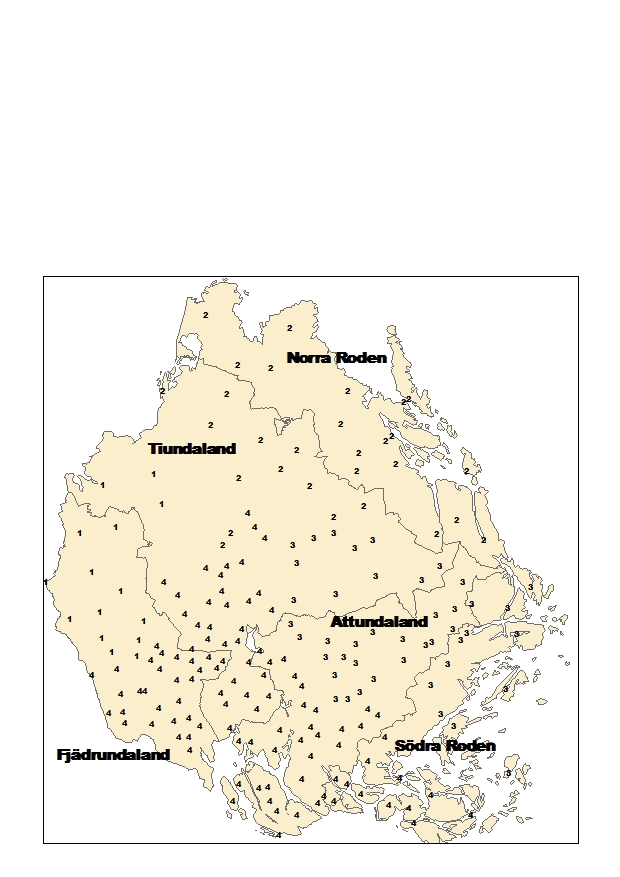
\includegraphics[height=.5\textheight]{figures/45_Kruuse}
\caption{Kruuse’s dialect areas and the Upplandic folklands}
\label{map:40}
\end{figure}

 
\begin{figure}[h]
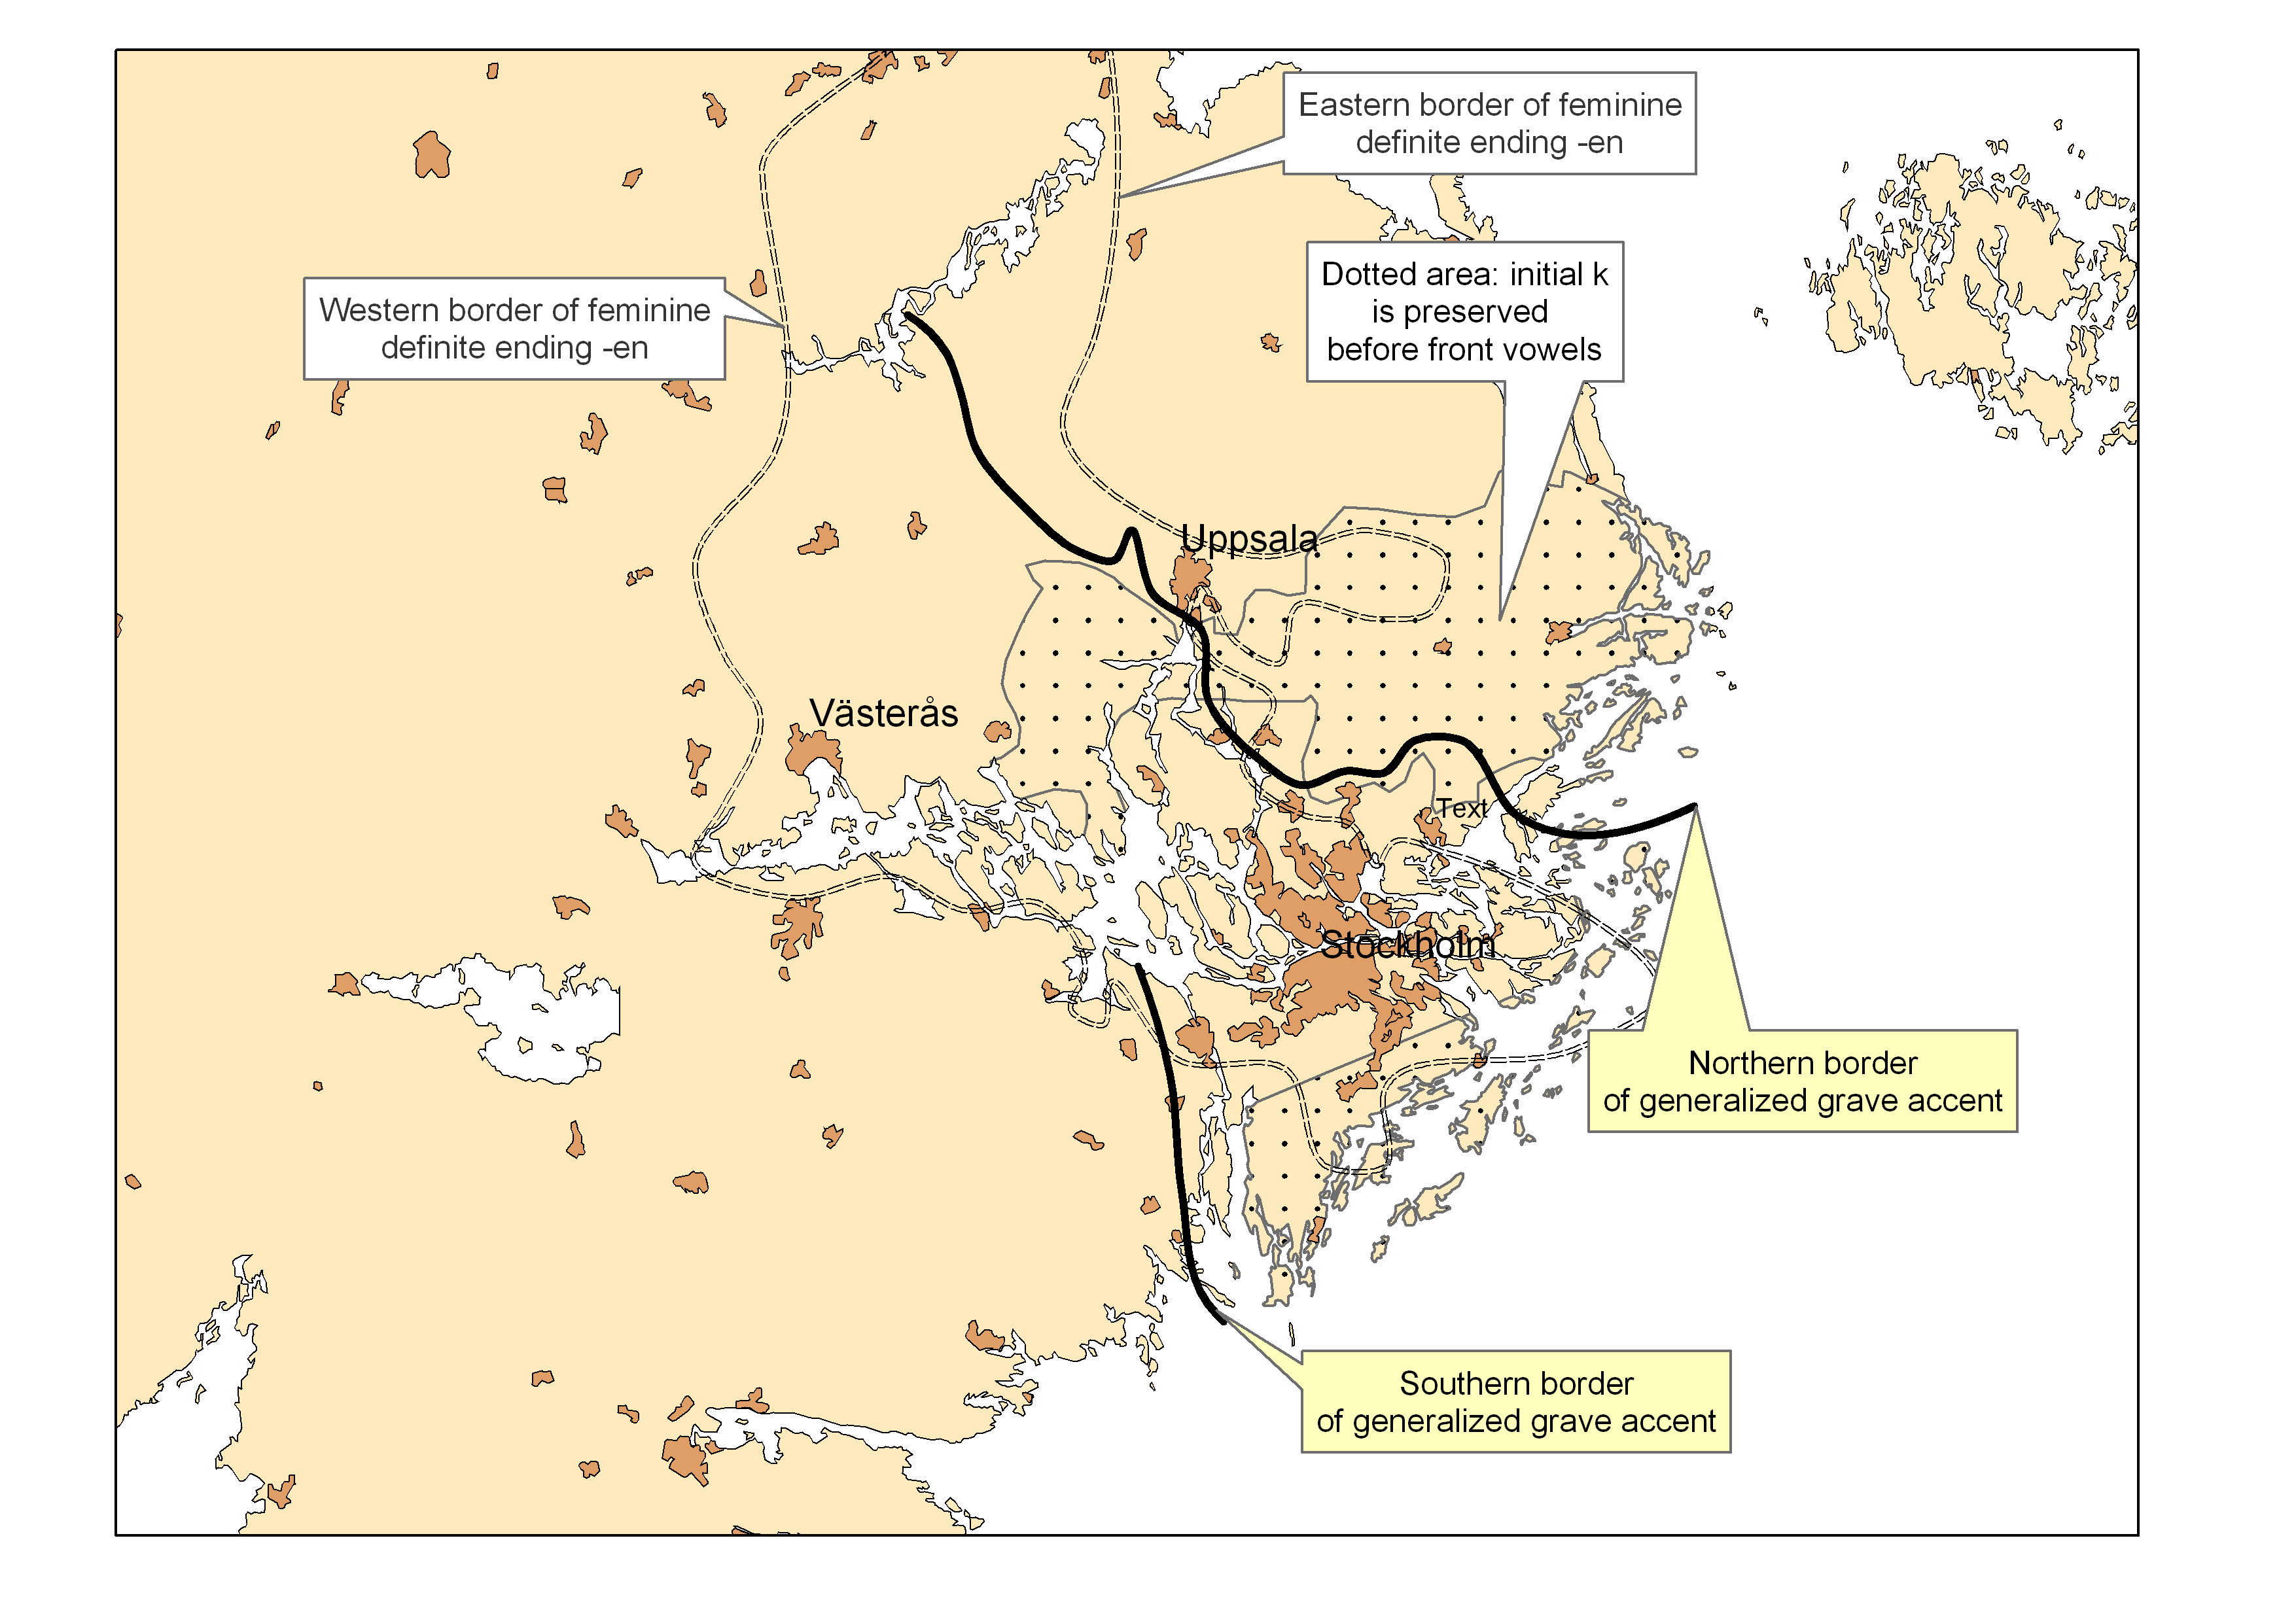
\includegraphics[height=.5\textheight]{figures/46_Mysterious}
\caption{Some mysterious dialect phenomena in the Mälar area.}
\label{map:41}
\end{figure}

 